% 2020 May 18 - THE MARTIAN ATMOSPHERIC BOUNDARY LAYER - https://agupubs.onlinelibrary.wiley.com/doi/10.1029/2010RG000351

% 2020 Oct 8 - ICC FOV = 120 deg, alpha = 10 * 0.82 mrad/px = 8.2 mrad = 0.14 deg
% https://mars.nasa.gov/insight/spacecraft/about-the-lander/#cameras
% https://www.nature.com/articles/s41467-020-14679-1
%
% D^{50%}_{\rm act} = 35 m

% Asurvey ~ (120 deg)(35 m)^2/(2*(0.14 deg)^2) = 3.8 km^2
% Seeing no dust devils means the areal density < 1/3.8 km^2 ~ 

% From Golombek+ (2020 - https://www.nature.com/articles/s41467-020-14679-1):
% A slope to the north limits the horizon to about 50 m away (Supplementary Fig. 5); it is topped by three rocks (The Pinnacles), and eolian bedforms (Dusty ridge) near the southwest rim of a ~100 m diameter degraded impact crater (Figs. 3–5). To the east-southeast (Fig. 4), the horizon extends about 400 m to the rim of a relatively fresh, ~100 m diameter impact crater (Sunrise) with large eolian bedforms on its rim (The Wave). The rim of a larger (460 m diameter), relatively fresh crater can be seen on the east-southeast horizon ~2.4 km away (Distant Crater in Fig. 6b).

%% Beginning of file 'sample63.tex'
%%
%% Modified 2019 June
%%
%% This is a sample manuscript marked up using the
%% AASTeX v6.3 LaTeX 2e macros.
%%
%% AASTeX is now based on Alexey Vikhlinin's emulateapj.cls 
%% (Copyright 2000-2015).  See the classfile for details.

%% AASTeX requires revtex4-1.cls (http://publish.aps.org/revtex4/) and
%% other external packages (latexsym, graphicx, amssymb, longtable, and epsf).
%% All of these external packages should already be present in the modern TeX 
%% distributions.  If not they can also be obtained at www.ctan.org.

%% The first piece of markup in an AASTeX v6.x document is the \documentclass
%% command. LaTeX will ignore any data that comes before this command. The 
%% documentclass can take an optional argument to modify the output style.
%% The command below calls the preprint style which will produce a tightly 
%% typeset, one-column, single-spaced document.  It is the default and thus
%% does not need to be explicitly stated.
%%
%%
%% using aastex version 6.3
\usepackage{amsmath}
\usepackage{wrapfig}
\documentclass{aastex63}

%% The default is a single spaced, 10 point font, single spaced article.
%% There are 5 other style options available via an optional argument. They
%% can be invoked like this:
%%
%% \documentclass[arguments]{aastex63}
%% 
%% where the layout options are:
%%
%%  twocolumn   : two text columns, 10 point font, single spaced article.
%%                This is the most compact and represent the final published
%%                derived PDF copy of the accepted manuscript from the publisher
%%  manuscript  : one text column, 12 point font, double spaced article.
%%  preprint    : one text column, 12 point font, single spaced article.  
%%  preprint2   : two text columns, 12 point font, single spaced article.
%%  modern      : a stylish, single text column, 12 point font, article with
%% 		  wider left and right margins. This uses the Daniel
%% 		  Foreman-Mackey and David Hogg design.
%%  RNAAS       : Preferred style for Research Notes which are by design 
%%                lacking an abstract and brief. DO NOT use \begin{abstract}
%%                and \end{abstract} with this style.
%%
%% Note that you can submit to the AAS Journals in any of these 6 styles.
%%
%% There are other optional arguments one can invoke to allow other stylistic
%% actions. The available options are:
%%
%%   astrosymb    : Loads Astrosymb font and define \astrocommands. 
%%   tighten      : Makes baselineskip slightly smaller, only works with 
%%                  the twocolumn substyle.
%%   times        : uses times font instead of the default
%%   linenumbers  : turn on lineno package.
%%   trackchanges : required to see the revision mark up and print its output
%%   longauthor   : Do not use the more compressed footnote style (default) for 
%%                  the author/collaboration/affiliations. Instead print all
%%                  affiliation information after each name. Creates a much 
%%                  longer author list but may be desirable for short 
%%                  author papers.
%% twocolappendix : make 2 column appendix.
%%   anonymous    : Do not show the authors, affiliations and acknowledgments 
%%                  for dual anonymous review.
%%
%% these can be used in any combination, e.g.
%%
%% \documentclass[twocolumn,linenumbers,trackchanges]{aastex63}
%%
%% AASTeX v6.* now includes \hyperref support. While we have built in specific
%% defaults into the classfile you can manually override them with the
%% \hypersetup command. For example,
%%
%% \hypersetup{linkcolor=red,citecolor=green,filecolor=cyan,urlcolor=magenta}
%%
%% will change the color of the internal links to red, the links to the
%% bibliography to green, the file links to cyan, and the external links to
%% magenta. Additional information on \hyperref options can be found here:
%% https://www.tug.org/applications/hyperref/manual.html#x1-40003
%%
%% Note that in v6.3 "bookmarks" has been changed to "true" in hyperref
%% to improve the accessibility of the compiled pdf file.
%%
%% If you want to create your own macros, you can do so
%% using \newcommand. Your macros should appear before
%% the \begin{document} command.
%%
\newcommand{\vdag}{(v)^\dagger}
\newcommand\aastex{AAS\TeX}
\newcommand\latex{La\TeX}
\newcommand{\totalvortices}{990}
\newcommand{\maskedvortices}{44}
\newcommand{\largestDeltaPobs}{$\left( 8.9 \pm 0.2 \right)\,{\rm Pa}$}
\newcommand{\largestDeltaPobssol}{65}
\newcommand{\largestGammaobssol}{20}
\newcommand{\largestGammaobs}{$\left( 99 \pm 3 \right)\,{\rm s}$}
\newcommand{\agreeablevortices}{127}
\newcommand{\vorticeswithnowinds}{56}

%% Reintroduced the \received and \accepted commands from AASTeX v5.2
\received{June 1, 2019}
\revised{January 10, 2019}
\accepted{\today}
%% Command to document which AAS Journal the manuscript was submitted to.
%% Adds "Submitted to " the argument.
\submitjournal{PSJ}

%% For manuscript that include authors in collaborations, AASTeX v6.3
%% builds on the \collaboration command to allow greater freedom to 
%% keep the traditional author+affiliation information but only show
%% subsets. The \collaboration command now must appear AFTER the group
%% of authors in the collaboration and it takes TWO arguments. The last
%% is still the collaboration identifier. The text given in this
%% argument is what will be shown in the manuscript. The first argument
%% is the number of author above the \collaboration command to show with
%% the collaboration text. If there are authors that are not part of any
%% collaboration the \nocollaboration command is used. This command takes
%% one argument which is also the number of authors above to show. A
%% dashed line is shown to indicate no collaboration. This example manuscript
%% shows how these commands work to display specific set of authors 
%% on the front page.
%%
%% For manuscript without any need to use \collaboration the 
%% \AuthorCollaborationLimit command from v6.2 can still be used to 
%% show a subset of authors.
%
%\AuthorCollaborationLimit=2
%
%% will only show Schwarz & Muench on the front page of the manuscript
%% (assuming the \collaboration and \nocollaboration commands are
%% commented out).
%%
%% Note that all of the author will be shown in the published article.
%% This feature is meant to be used prior to acceptance to make the
%% front end of a long author article more manageable. Please do not use
%% this functionality for manuscripts with less than 20 authors. Conversely,
%% please do use this when the number of authors exceeds 40.
%%
%% Use \allauthors at the manuscript end to show the full author list.
%% This command should only be used with \AuthorCollaborationLimit is used.

%% The following command can be used to set the latex table counters.  It
%% is needed in this document because it uses a mix of latex tabular and
%% AASTeX deluxetables.  In general it should not be needed.
%\setcounter{table}{1}

%%%%%%%%%%%%%%%%%%%%%%%%%%%%%%%%%%%%%%%%%%%%%%%%%%%%%%%%%%%%%%%%%%%%%%%%%%%%%%%%
%%
%% The following section outlines numerous optional output that
%% can be displayed in the front matter or as running meta-data.
%%
%% If you wish, you may supply running head information, although
%% this information may be modified by the editorial offices.
\shorttitle{Vortices and Meteorology from InSight}
\shortauthors{Jackson}
%%
%% You can add a light gray and diagonal water-mark to the first page 
%% with this command:
%% \watermark{text}
%% where "text", e.g. DRAFT, is the text to appear.  If the text is 
%% long you can control the water-mark size with:
%% \setwatermarkfontsize{dimension}
%% where dimension is any recognized LaTeX dimension, e.g. pt, in, etc.
%%
%%%%%%%%%%%%%%%%%%%%%%%%%%%%%%%%%%%%%%%%%%%%%%%%%%%%%%%%%%%%%%%%%%%%%%%%%%%%%%%%
\graphicspath{{./}{figures/}}
%% This is the end of the preamble.  Indicate the beginning of the
%% manuscript itself with \begin{document}.

\begin{document}

\title{Inferring Vortex and Meteorological Statistics from InSight}

%% LaTeX will automatically break titles if they run longer than
%% one line. However, you may use \\ to force a line break if
%% you desire. In v6.3 you can include a footnote in the title.

%% A significant change from earlier AASTEX versions is in the structure for 
%% calling author and affiliations. The change was necessary to implement 
%% auto-indexing of affiliations which prior was a manual process that could 
%% easily be tedious in large author manuscripts.
%%
%% The \author command is the same as before except it now takes an optional
%% argument which is the 16 digit ORCID. The syntax is:
%% \author[xxxx-xxxx-xxxx-xxxx]{Author Name}
%%
%% This will hyperlink the author name to the author's ORCID page. Note that
%% during compilation, LaTeX will do some limited checking of the format of
%% the ID to make sure it is valid. If the "orcid-ID.png" image file is 
%% present or in the LaTeX pathway, the OrcID icon will appear next to
%% the authors name.
%%
%% Use \affiliation for affiliation information. The old \affil is now aliased
%% to \affiliation. AASTeX v6.3 will automatically index these in the header.
%% When a duplicate is found its index will be the same as its previous entry.
%%
%% Note that \altaffilmark and \altaffiltext have been removed and thus 
%% can not be used to document secondary affiliations. If they are used latex
%% will issue a specific error message and quit. Please use multiple 
%% \affiliation calls for to document more than one affiliation.
%%
%% The new \altaffiliation can be used to indicate some secondary information
%% such as fellowships. This command produces a non-numeric footnote that is
%% set away from the numeric \affiliation footnotes.  NOTE that if an
%% \altaffiliation command is used it must come BEFORE the \affiliation call,
%% right after the \author command, in order to place the footnotes in
%% the proper location.
%%
%% Use \email to set provide email addresses. Each \email will appear on its
%% own line so you can put multiple email address in one \email call. A new
%% \correspondingauthor command is available in V6.3 to identify the
%% corresponding author of the manuscript. It is the author's responsibility
%% to make sure this name is also in the author list.
%%
%% While authors can be grouped inside the same \author and \affiliation
%% commands it is better to have a single author for each. This allows for
%% one to exploit all the new benefits and should make book-keeping easier.
%%
%% If done correctly the peer review system will be able to
%% automatically put the author and affiliation information from the manuscript
%% and save the corresponding author the trouble of entering it by hand.

\correspondingauthor{Brian Jackson}
\email{bjackson@boisestate.edu}

\author[0000-0002-9495-9700]{Brian Jackson}
\author{Justin Crevier}
\author{Michelle Szurgot}
\author{Ryan Battin}
\affiliation{Department of Physics\\ 
Boise State University\\ 
1910 University Drive, Boise ID 83725-1570 USA}

%% Note that the \and command from previous versions of AASTeX is now
%% depreciated in this version as it is no longer necessary. AASTeX 
%% automatically takes care of all commas and "and"s between authors names.

%% AASTeX 6.3 has the new \collaboration and \nocollaboration commands to
%% provide the collaboration status of a group of authors. These commands 
%% can be used either before or after the list of corresponding authors. The
%% argument for \collaboration is the collaboration identifier. Authors are
%% encouraged to surround collaboration identifiers with ()s. The 
%% \nocollaboration command takes no argument and exists to indicate that
%% the nearby authors are not part of surrounding collaborations.

%% Mark off the abstract in the ``abstract'' environment. 
\begin{abstract}
The InSight Mission has operated on the surface of Mars for nearly two Earth years, returning hundreds of sols worth of data, including detections of the first Marsquakes. The lander also deployed an exquisitely sensitive meteorological instrument package to assess the influence of the atmosphere on the geophysical measurements, as well as imaging cameras to monitor both instrument deployment and local surface activity. In addition to their relevance to InSight geoscience, these latter instruments have detected a variety of boundary layer phenomena, including an unprecedented number of encounters with small-scale vortices. These vortices register as short-lived ($<$ tens of seconds), negative ($<$ a few \% ambient) pressure excursions in the barometric time-series collected by InSight. These vortices closely resemble dust devils, which largely shape climate and air quality on Mars where they are widespread. Puzzlingly, although InSight detected more than 9,000 such vortices and collected hundreds of mid-day images (as reported in \citealp{2020arXiv200501134S}), no active dust devils were imaged -- apparently, all the vortices were dustless. In spite of the lack of dust devil detections, we can leverage the vortex detections and InSight’s daily wind speed measurements to learn about the boundary layer processes that create dust devils. Such an analysis could even help us optimize our vortex detection strategies. In this study, we will discuss our own analysis of InSight’s meteorological data to assess the statistics of vortex and dust devil activity. Comparing these results to InSight’s imagery and space-based observations of the InSight landing site, we can also statistically infer the maximum dust-loading allowed for nearby dust devils. 
\end{abstract}

%% Keywords should appear after the \end{abstract} command. 
%% See the online documentation for the full list of available subject
%% keywords and the rules for their use.
\keywords{editorials, notices --- 
miscellaneous --- catalogs --- surveys}

%% From the front matter, we move on to the body of the paper.
%% Sections are demarcated by \section and \subsection, respectively.
%% Observe the use of the LaTeX \label
%% command after the \subsection to give a symbolic KEY to the
%% subsection for cross-referencing in a \ref command.
%% You can use LaTeX's \ref and \label commands to keep track of
%% cross-references to sections, equations, tables, and figures.
%% That way, if you change the order of any elements, LaTeX will
%% automatically renumber them.
%%
%% We recommend that authors also use the natbib \citep
%% and \citet commands to identify citations.  The citations are
%% tied to the reference list via symbolic KEYs. The KEY corresponds
%% to the KEY in the \bibitem in the reference list below. 

\section{Introduction} \label{sec:Introduction}

% 2020 May 16 - Discuss how Greeley et al. (2006) spotted and analyzed dust devils.

% \citet{2010Icar..206..306N} report a dust flux $Q$ that depends on the pressure deficit at the center of a vortex $\Delta P$ as
% \begin{equation}
%     Q = \left(5.79\times10^{-8} {\rm kg\ m^{-2}\ s^{-1}} \right) \left( \Delta P/{\rm Pa}\right)^{3.40}.
%     \label{eqn:Neakrase_dust_flux}
% \end{equation}
% \begin{figure}
%     \centering
%     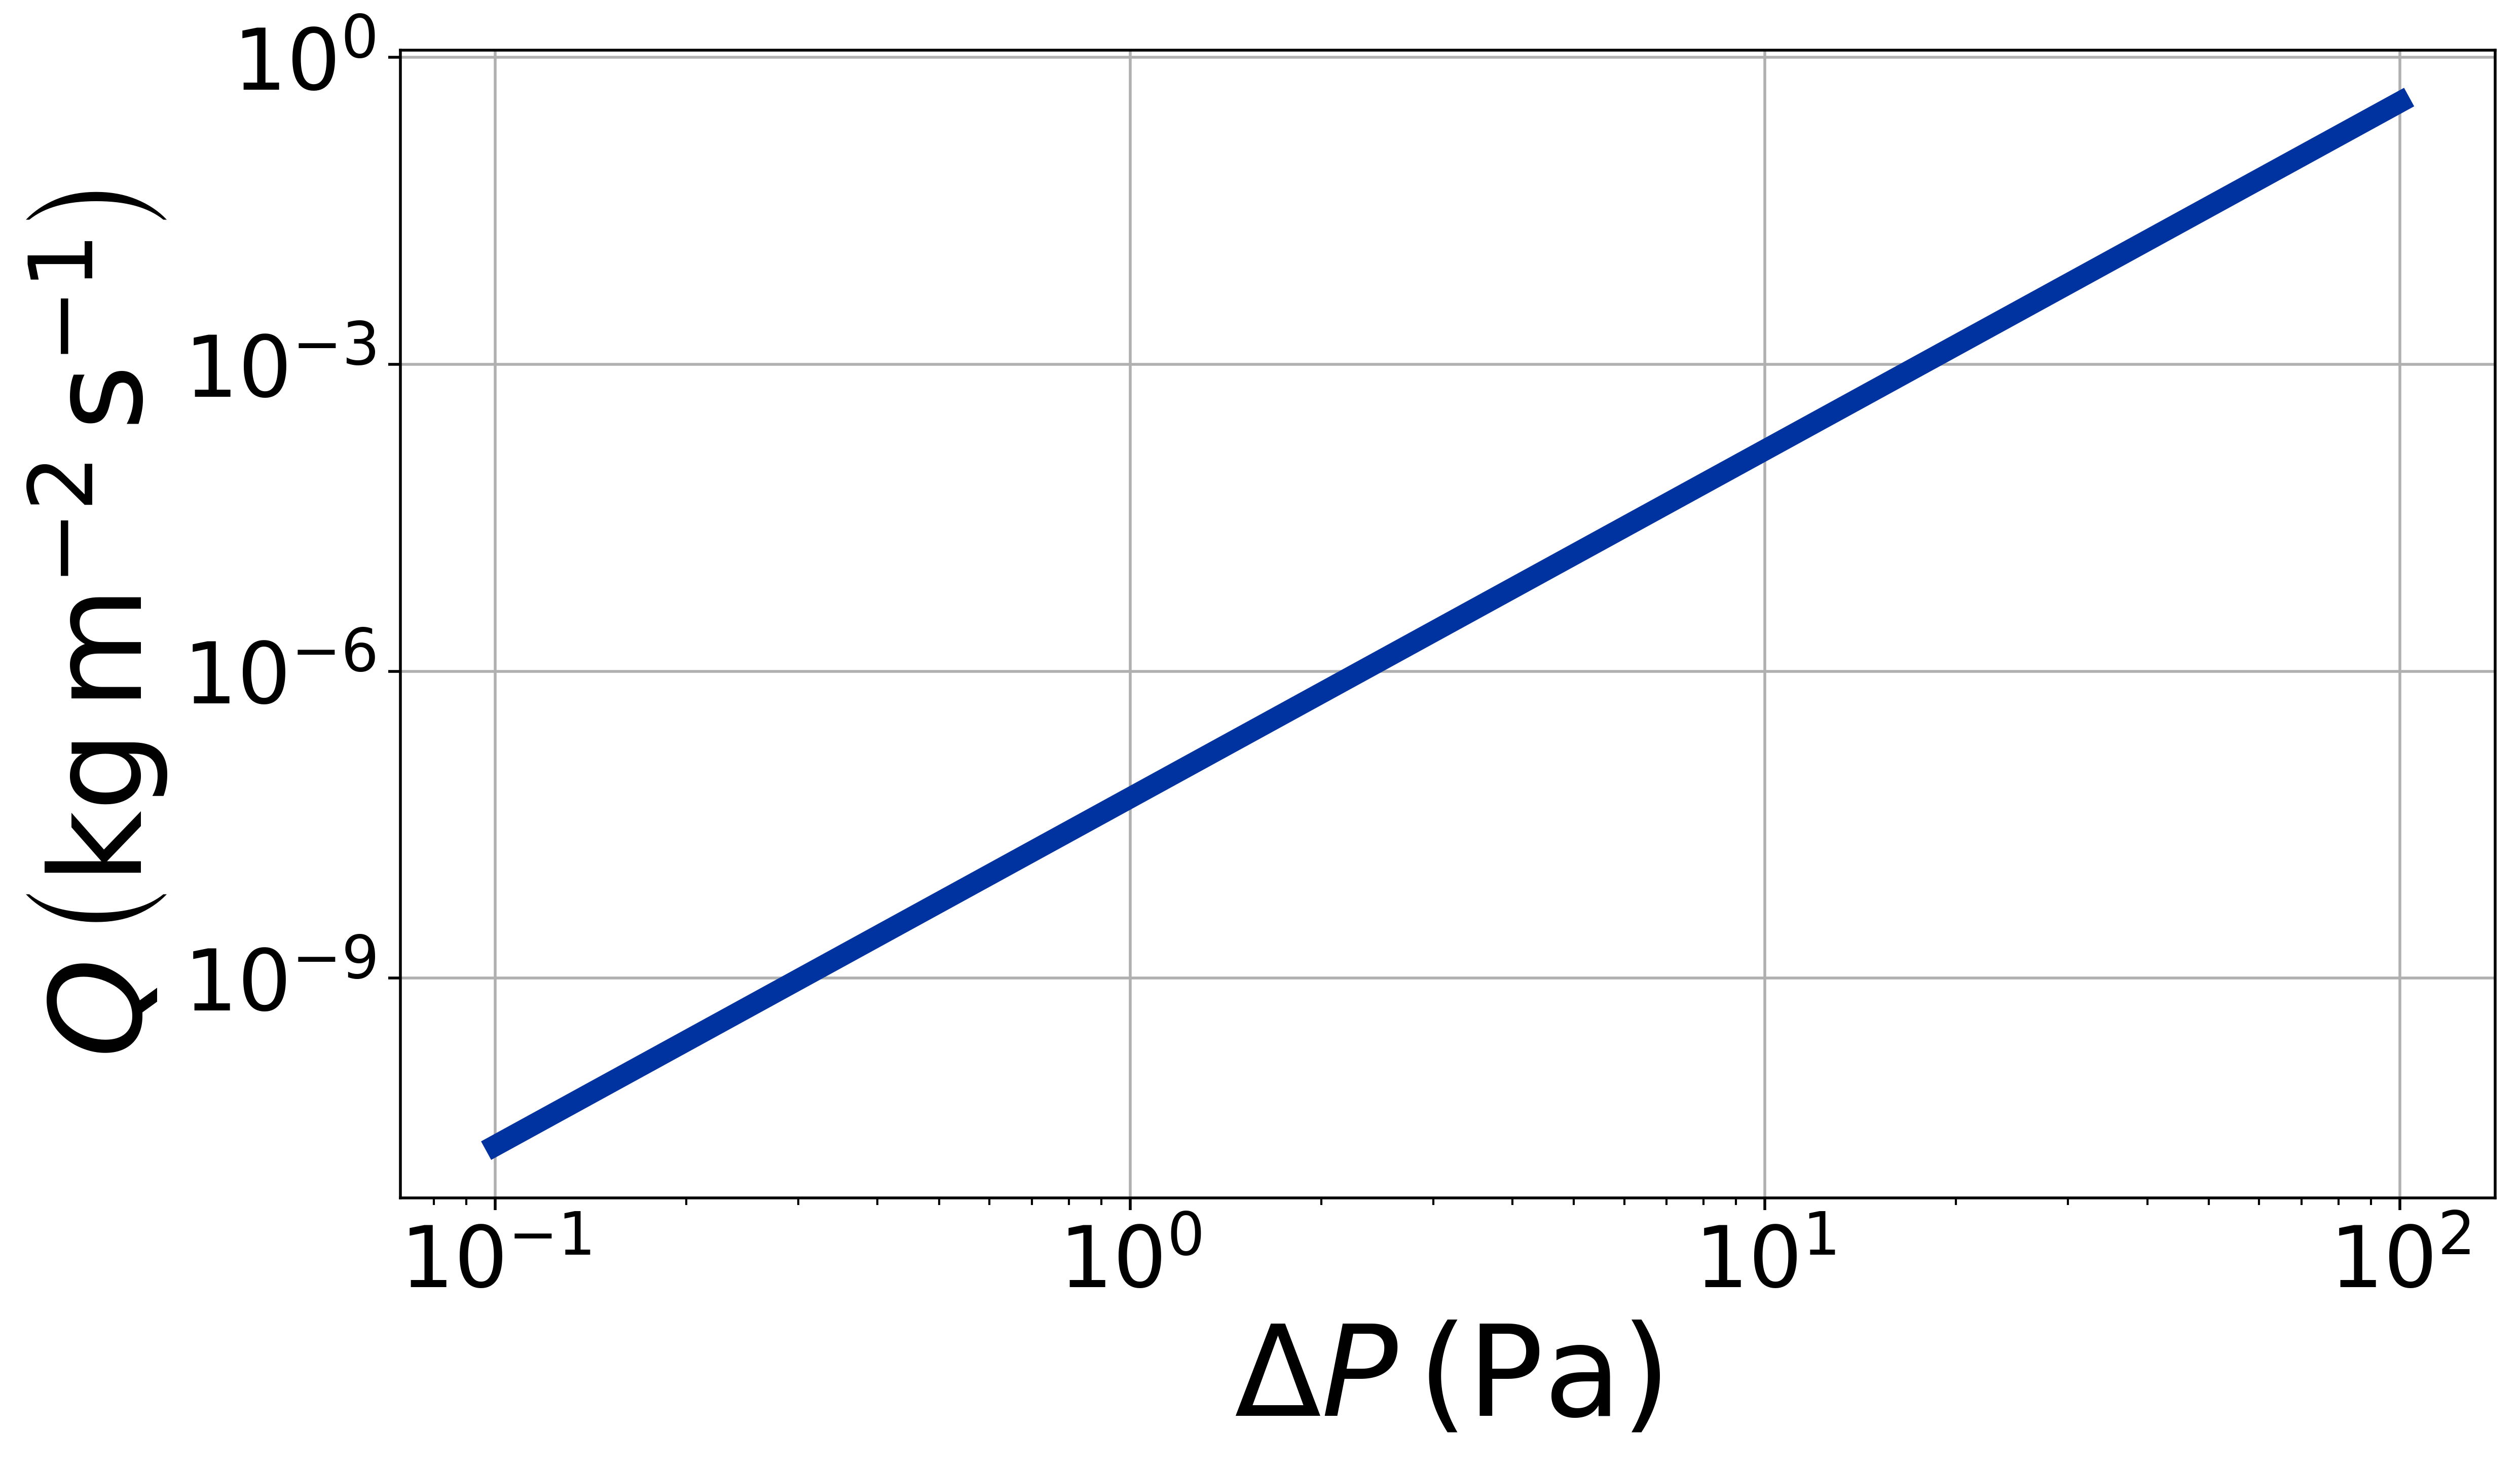
\includegraphics[width=\textwidth]{figures/Q_vs_Delta-P.png}
%     \caption{Dust flux $Q$ as a function of the pressure dip at the center of a lab-generated vortex $\Delta P$, as reported in \citet{2010Icar..206..306N}.}
%     \label{fig:Neakrase_dust_flux}
% \end{figure}

% XXX Where did InSight land? XXX

The InSight spacecraft landed on Elysium Planitia ($4.5^\circ$ N, $135.6^\circ$ E) on 2018 Nov 28, carrying suites both of geophysical \citep{} and meteorological instruments \citep{}. Since wind gusts and other atmospheric boundary layer phenomena can perturb the geophysical measurments, particularly the seismometry, these meteorological instruments 

An in-situ survey could be tailored to test ideas about dust devils. 

\citet{1998JAtS...55.3244R} proposed the ``dust devil activity'' (DDA) parameter, the product of the surface sensible heat flux and a thermodynamic efficiency related to the depth of the planetary boundary layer. During the martian day, the heat flux and boundary layer depth increase as insolation heats the surface. \citet{2019JGRE..124.3442N} conducted large eddy simulations of the environment in and around Gale Crater to assess the DDA, along with other micrometeorological parameters as a function of position and time-of-day. The study then compared those model predictions to the rate at which short-lived dips appeared in the barometric time-series, likely indicative of vortex encounters. The study found that the frequency of vortex encounters scaled with DDA.

However, in \citet{1998JAtS...55.3244R}, the actual relationship between DDA and dust devil properties remains unclear: whether a larger DDA translates into a higher frequency of dust devils, more large dust devils, more vigorous dust devils. The results in \citet{2019JGRE..124.3442N} suggest the frequency at least increases with DDA, but it is not clear whether the increased frequency arose from higher surface winds (which would more quickly advect vortices past the sensor). Also unknown was whether the detected vortices exhibited deeper pressure excursions or more vigorous winds. A tailored imaging survey for dust devils, especially combined with a meteorological dataset, could disentangle the influence of DDA on dust devil properties. 

The detailed influence of dust devils on Mars' atmosphere likewise remain obscure. 

For this study, we will consider two types of dust devil detections and analyses: the first involves dust devils far enough from the instrument suite that they are analyzed using only imagery; the second involves dust devils that pass over the instruments. The latter detection has the potential to more directly elucidate the pressure, temperature, and wind structures within a dust devil, as well as the dust abundance but requires a rare encounter at a distance from a devil's center not much more than the eyewall diameter. The former detection may also reveal the dust content but indirectly, via a analysis of the image contrast; however such detections are much more common since they can be made out to the resolution of the imaging system and may therefore provide a more robust assessment of dust devil statistics. 

% Define areal density N

The atmospheric influence of a dust devil population depends on the areal density of dust devil occurrence and the dust flux for each. Thus, accurately assessing that influence requires accurate estimates of the both.

\section{Time-Series Analysis}
In this section, we describe our analysis of the pressure and wind speed time-series. We first describe the data themselves. Next, we discuss our search for vortex signals using the pressure time-series and explore its biases and completeness, which \citet{2015JGRE..120..401J} showed are important for inferring the underlying occurrence rates from the observations. Next, we describe how we modeled the pressure and wind speed profiles of individual vortex encounters, which, as we show, allows us to determine not just the observed pressure and wind excursions but also to infer the encounter geometries and intrinsic vortex parameters \citep[cf.][]{2016Icar..271..326L}. We also discuss the statistical distributions and correlations of vortex parameters and compare them to predictions and previous work. 

\subsection{Data}
The pressure measurements from the APSS are taken at $20\, {\rm Hz}$ with a nominal precision of $50\, {\rm mPa\ Hz^{−1/2}}$ or better, much higher frequency and precision than available from some previous Mars landers \citep[e.g.,][]{2010JGRE..115.0E16E}. As we discuss below, turbulent excursions given an effective scatter in the pressure data between $0.2$ and $0.5\,{\rm Pa}$, depending on ambient conditions. In any case, such specs make APSS ideal for studying turbulent signals in the martian boundary layer \citep{2018SSRv..214..109S}. APSS has measured pressures nearly non-stop since sol 14 of the mission, and for our study, we considered data up through sol 477 of the mission, amounting to almost 82 GB. The data are available from NASA's Atmosphere's PDS Node - \url{https://atmos.nmsu.edu/data_and_services/atmospheres_data/INSIGHT/insight.html}. PDS provides several sets of data files for APSS, and we used the CSV files in the ``data\_calibrated'' folder.

Wind data come from the TWINS instrument, the sensors for which sit on booms located on the InSight platform and facing opposite directions about a meter above the solar panels \citep{2020NatGe..13..190B}. TWINS acquires data at $0.1\, {\rm Hz}$ and $1\, {\rm Hz}$ with an accuracy of $1\, {\rm m\ s^{-1}}$ for wind speed and $22.5^\circ$ for wind direction. Since the wind direction data give constraints that are, in principle, redundant and less robust than the wind speed data, we do not include the direction data in our analysis. TWINS has also provided a dataset spanning nearly the whole time from sol 14 to 477, amounting to more than 18 GB. For our work here, we focus on the higher time resolution ($1\, {\rm Hz}$) wind data, which is more limited in extent, often only spanning the mid- to late afternoon for a given sol. The wind measurements involve modeled reconstructions, as described in  \citep{Banfield2018}, and we used the cSV files in the ``data\_derived'' folder. The higher time resolution files are labeled as ``modelevent''. (The lower resolution files are labeled as ``model'').

Vortex encounters can also produce excursions in ambient temperature (as the warm core passes over the sensor) \citep{2016SSRv..203...39M}, and APSS does return air temperature data. However, we do not model these time-series since the temperature data show small or negligible excursions during the encounters. In any case, the temperatures would be expected to simply mirror the pressure excursions \citep{2016Icar..271..326L}.

\subsection{Searching for Vortex Encounters and Fitting Pressure Profiles}
Both the pressure and wind speed data exhibit turbulent excursions that constitute a source of non-Gaussian noise and complicate our search for vortex encounters. However, the pressure data are both more plentiful and less affected by these excursions, so we search for encounters using the pressure time-series. This approach replicates many prior studies, including previous analyses of InSight data \citep{2020arXiv200501134S, 2021Icar..35514119L}. Figure \ref{fig:data_conditioning_and_fit} depicts our search process in graphical form, and panel (a) shows the raw pressure time-series for sol 392, a representative sol. The vertical dashed orange lines show the vortex signals, whose detection we describe next. Any time-series analysis scheme will unavoidably involve selection effects that can skew the recovered population of signals \citep{2018Icar..299..166J}, and we explore biases of our detection scheme and how those influence the final recovered population of vortices in the Appendix (Section \ref{sec:Vortex Recovery Statistics}). 

To suppress longer-term signals and facilitate detection of the vortices, we apply a mean boxcar filter with a window size $W$ before sifting the data for vortices. Figure \ref{fig:data_conditioning_and_fit}(b) shows the resulting detrended time-series $\Delta P$. Based on the analysis described in the Appendix (Section \ref{sec:Vortex Recovery Statistics}), we chose $W = 3000\,{\rm s}$. 

Next, we employ a matched filter approach \citep[][ch.~13]{Press2007} using a normalized Lorentzian profile with a known FWHW, $\Gamma$; that is, we march a Lorentzian profile, point-by-point, across the time series, convolving it with the time-series. Based on our analysis in the Appendix (Section \ref{sec:Vortex Recovery Statistics}), we chose $\Gamma = 1\,{\rm s}$. This process produces the equivalent of a spectrum, with large positive spikes when the filter encounters other Lorentzian-like signals. We subtract the median value from this raw spectrum and then normalize it by the standard deviation (as estimated by $1.4826\ \times$ the median absolute deviation -- \citealp{doi:10.1080/01621459.1993.10476408}). We consider peaks rising above the detection threshold of 5 to be possible vortices. Figure \ref{fig:data_conditioning_and_fit}(c) shows this normalized spectrum for the time-series in panel (b), along with the peaks raising above $F \ast P = 5$ (vertical dashed orange lines). 

Finally, considering the original, undetrended time-series (e.g., Figure \ref{fig:data_conditioning_and_fit}(a)), we use the Levenberg-Marquardt algorithm \citep[cf.][]{Press2007} to fit the time-series in a window 30-FWHMs wide around each vortex signal. As in previous work \citep[e.g.,][]{2016JGRE..121.1514K}, we assume the pressure structures of vortices are accurately represented by a steady-state modified Lorentzian profile,

\begin{equation}
    \Delta P(r) = -\frac{\Delta P_{\rm act}}{1 + \left( \frac{r}{D_{\rm act}/2} \right)^2}\label{eqn:radial_lorentzian_profile}
\end{equation}
where $r$ the radial distance of the InSight sensors from the vortex center, $P_{\rm act}$ the pressure excursion at the vortex center, and $D_{\rm act}$ is taken as the vortex diameter. As a function of time $t$, $r(t)$ is given by
\begin{equation}
    r(t) = \sqrt{b^2 + U^2 \left( t - t_0 \right)^2}.\label{eqn:radial_distance}
\end{equation}
where $t_0$ is the time of closest approach. This scheme assumes the vortex travels past the sensor on a linear trajectory with a unidirectional and constant velocity $U$ (at least during the course of a single encounter). The closest approach distance between the vortex center and the InSight sensors $b$ is usually greater than zero. As a result, the minimum observed in the pressure time-series $\Delta P_{\rm obs}$ is not usually as deep as the actual pressure excursion at the vortex center \citep{2018Icar..299..166J, 2019Icar..317..209K}. The pressure time-series for a vortex encounter can therefore be represented by 
\begin{equation}
    \Delta P(t) = \frac{-\Delta P_{\rm obs}}{1 + \left( \frac{ t - t_0 }{\Gamma_{\rm obs}/2} \right)^2},\label{eqn:Lorentzian_profile}
\end{equation}
where $\Gamma_{\rm obs}$ is the observed profile full-width/half-max (FWHM). With these definitions, $\Gamma_{\rm obs} = U^{-1} \sqrt{D_{\rm act}^2 + \left( 2 b \right)^2}$. 

We fit this profile combined with a linear trend, returning best fit parameters $t_0$, $\Delta P_{\rm obs}$, and $\Gamma_{\rm obs}$, as well as the background slope and intercept. Fitting such a model to the original, undetrended data instead of the detrended time-series avoids the distorting effect of the boxcar filter on the vortex signal while taking into account any background trend. Figure \ref{fig:data_conditioning_and_fit}(d) shows such a fit (with the background intercept subtracted out). Section \ref{sec:Results} below presents the results from this analysis.

\begin{figure}
    \centering
    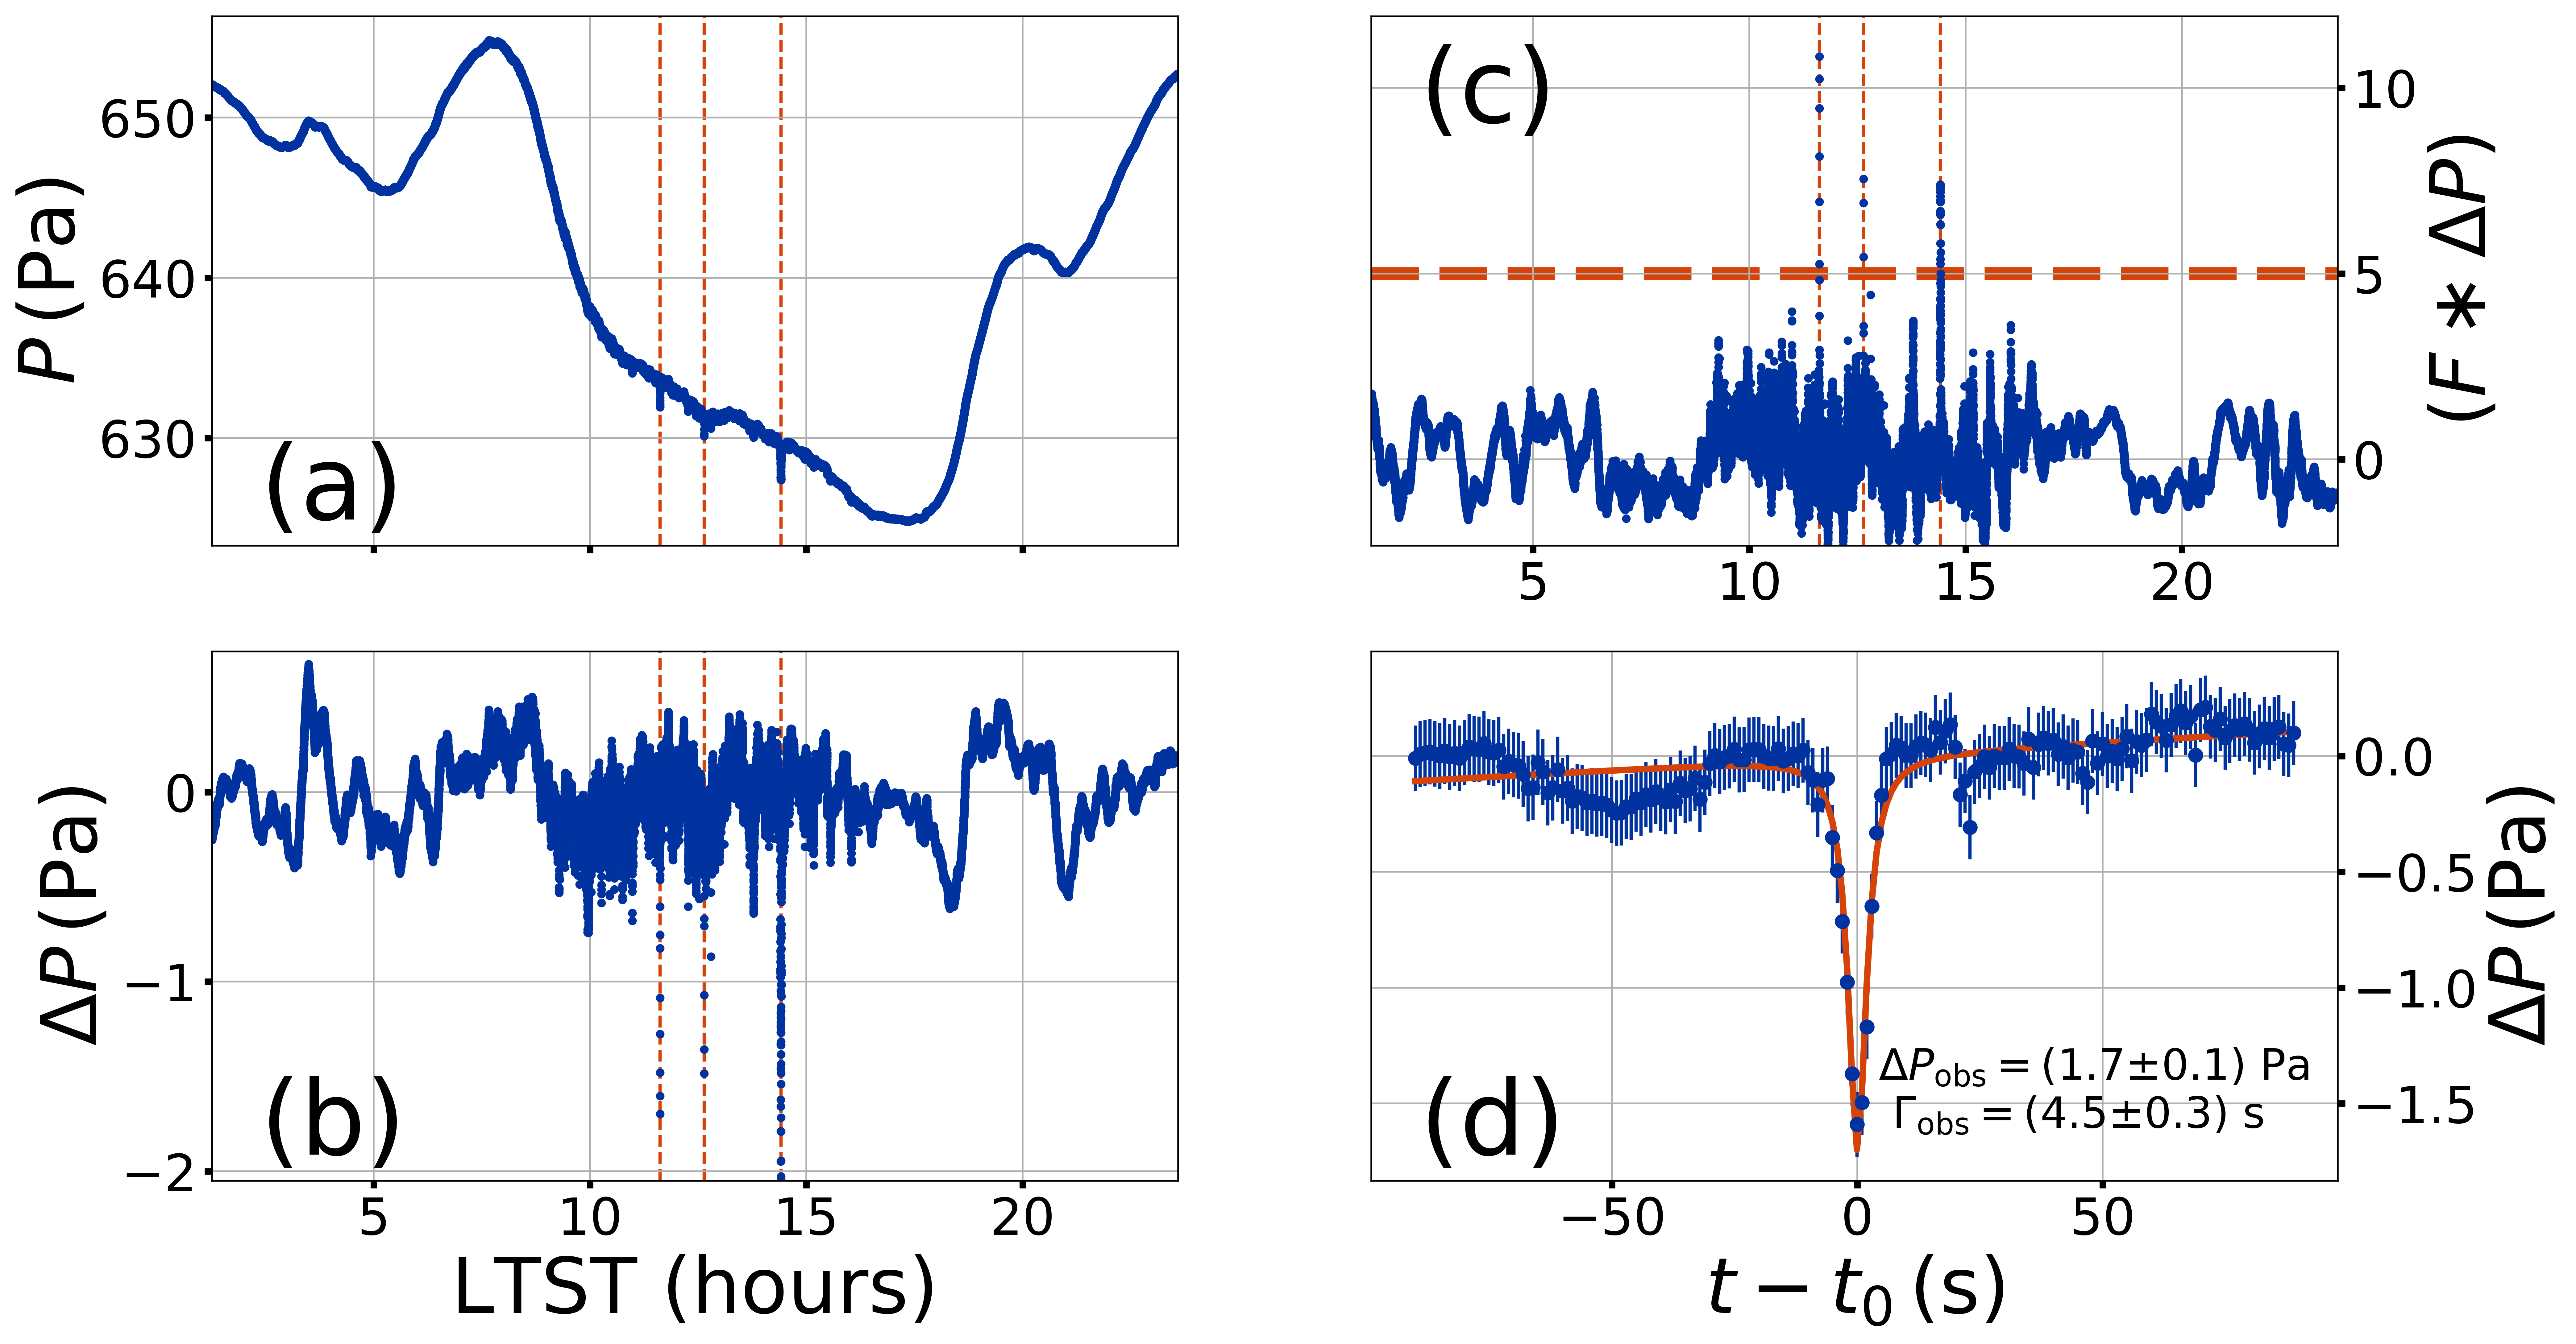
\includegraphics[width=\textwidth]{figures/data_conditioning_and_fit.png}
    \caption{(a) The pressure time-series for sol 392, as blue dots. The vertical orange lines highlight the detected vortex signals. (b) The time-series after application of the mean boxcar filter. Apparent by eye, the scatter in the time-series increases around mid-day. (c) Convolution of the matched filter with the time-series in (b). The horizontal dashed orange line shows the detection threshold of 5. (d) A model fit (solid orange line) to the deepest vortex discovered on sol 392, along with the model fit parameters -- each point's uncertainty is calculated via $1.4826\ \times$ the median absolute deviation in the window centered on that point.}
    \label{fig:data_conditioning_and_fit}
\end{figure}

\subsection{Fitting Wind Profiles}
\label{sec:Pressure and Wind Models}
To assess the intrinsic vortex properties and encounter geometries, we also fit wind speed profiles to the wind speed time-series that coincide in time with the peaks found by our search. The wind speed signal consists both of an ambient wind $U$ and the vortex wind $V(r)$, which is a function of radial distance (and therefore time). For the Rankine vortex model \citep{1991ExFl...11...73V}, $V(r)$ is given by
\begin{equation}
    V(r) = V_{\rm act} \frac{2 \left( \frac{r}{D_{\rm act}/2} \right) }{1 + \left( \frac{r}{D_{\rm act}/2} \right)^2},
\end{equation}
where $V_{\rm act}$ is the tangential wind speed at the vortex diameter. Similar to the pressure signal, a non-zero $b$ means the maximum wind speed encountered $V_{\rm obs}$ is less than the actual maximum at the vortex diameter. We model the observed vortex wind profile as
\begin{equation}
    V(r) = V_{\rm obs} \frac{\sqrt{1 + \left( U_1/b \right)^2 \left( t - t_0 \right)^2}}{1 + \left(\frac{t - t_0}{\Gamma_{\rm obs}/2}\right)^2},\label{eqn:wind_profile}
\end{equation}
where $U_1$ is the ambient wind speed before the encounter and which we take as the advective speed for the vortex. Strictly, this model breaks down for $b = 0$, but such an encounter is statistically unlikely \citep{2018Icar..299..166J}. Many of the wind signals exhibit a different ambient wind speed before the encounter ($U_1$) than after the encounter ($U_2$). Thus, the total wind speed observed $W(t)$ is the vector sum of the ambient wind and vortex wind, given by 
\begin{equation}
    W(t) = \left\{
    \begin{array}{ll}
            \sqrt{V^2 + 2 U_1 V \cos \theta + U_1^2}, & \left( t - t_0 \right) \leq 0\\
            \sqrt{V^2 + 2 U_2 V \cos \theta + U_2^2}, & \left( t - t_0 \right) > 0\\
    \end{array},\label{eqn:total_wind_speed}
\end{equation}
where $\cos \theta = b/\sqrt{b^2 + \left( U_{1/2} \right)^2\left( t - t_0 \right)^2}$. 

We fit the pressure and wind speed profiles for each encounter in two separate steps -- first, the pressure, then the wind speed. In so doing, we hold the $\Gamma_{\rm obs}$-value fixed from the pressure profile fit. Experimentation showed this approach most frequently gave reasonable results, and Figure \ref{fig:vortices_and_windspeed} shows several examples of the profile fits. 

As we show in Appendix \ref{sec:Inferring Encounter Geometries from the Pressure and Velocity Profiles}, we can estimate $\Delta P_{\rm act}$ and $V_{\rm act}$, along with the encounter distance $b$, from the observed parameters. To check this approach, we applied these models to many synthetic vortex encounters for a range of encounter geometries, vortex parameters, and time-series noise representative of the observed values. We found that, for encounters with $b \lesssim D_{\rm act}$, we were able to recover the assumed parameters to within 50\% for the majority of cases. For encounters farther than that, the signals were usually lost in the noise. Future work should explore more robust approaches. In what follows, we initially retain all vortices detected, regardless of their best-fit $b$-values, since the best-fit $\Delta P_{\rm obs}$- and $\Gamma_{\rm obs}$ are independent of $b$, but for results later on that depend on $b$, we dropped those vortices with $b > D_{\rm act}$. That transition is clearly indicated in the narrative below.

\begin{figure}
\centering
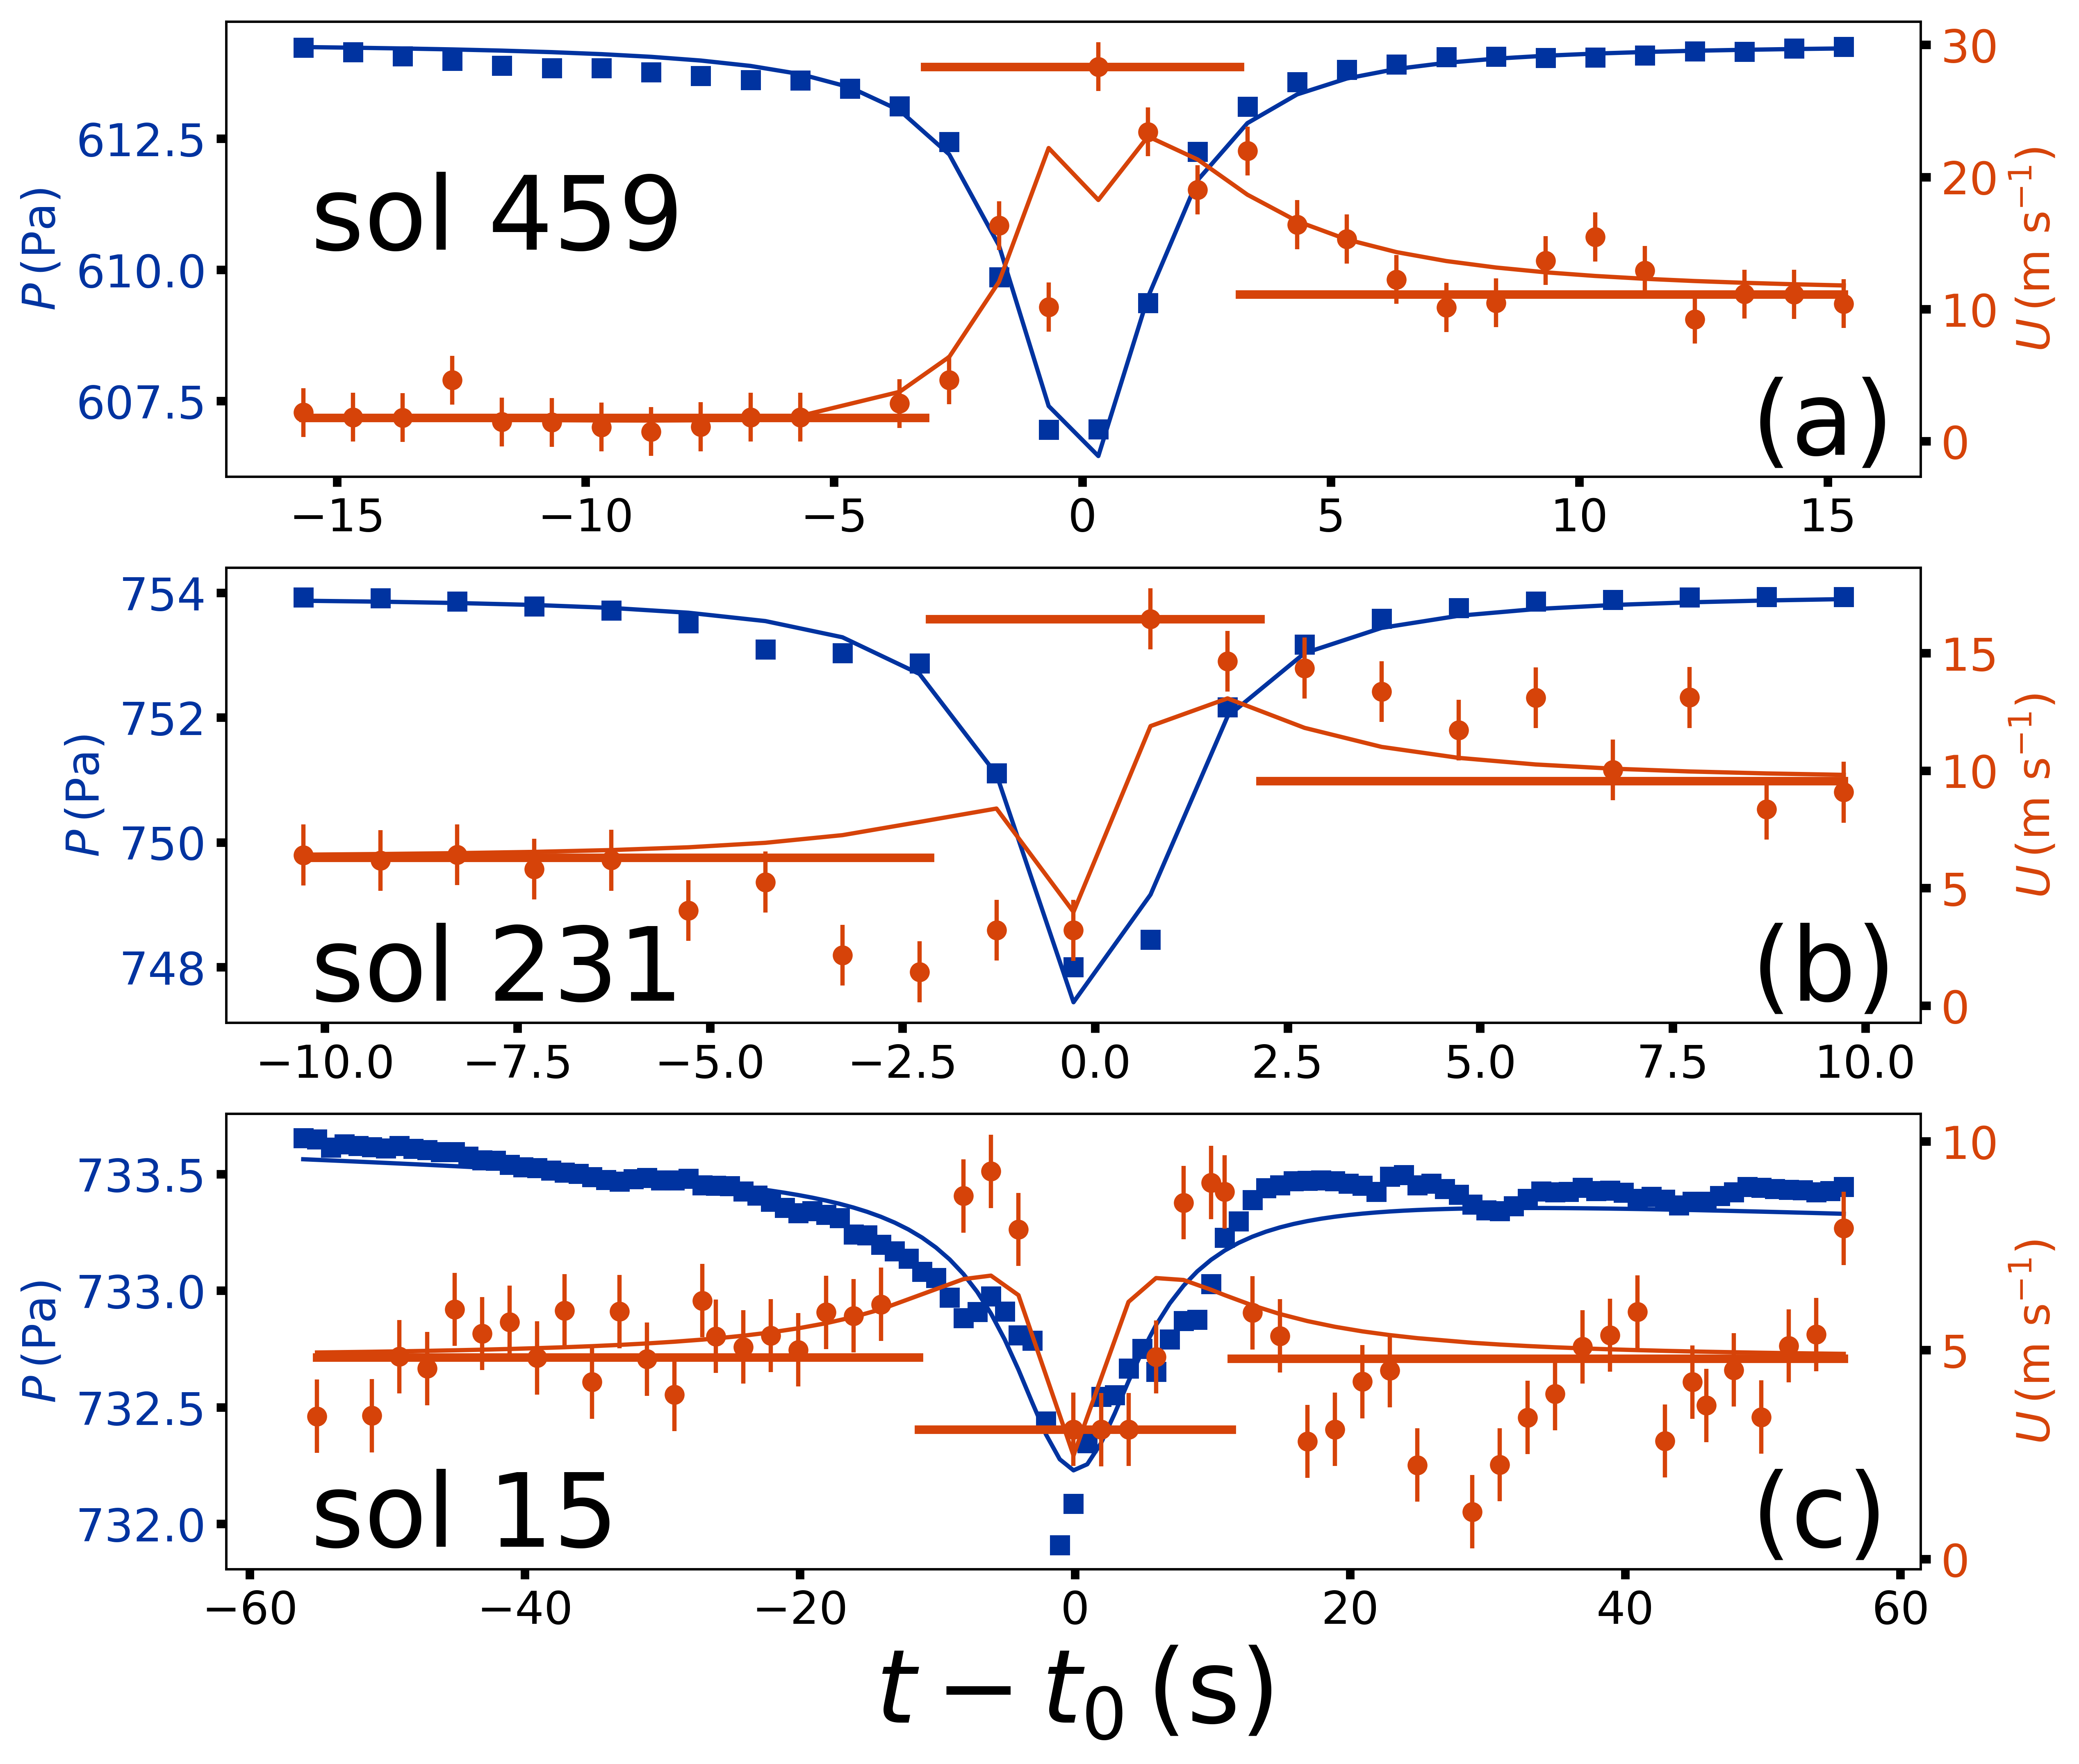
\includegraphics[width=0.48\textwidth]{figures/vortices_and_windspeed.png}
\caption{Pressure data (blue dots) and models (blue lines) and horizontal windspeed data (orange dots) and models. \label{fig:vortices_and_windspeed}}
\end{figure}

\section{Results}
\label{sec:Results}
Figure \ref{fig:DeltaPobs_vs_Gammaobs}(a) shows our collection of best-fit $\Gamma_{\rm obs}$- and $\Delta P_{\rm obs}$-values, along with their respective cumulative histograms. Inspecting an initial tranche of detections by-hand, we found that vortices with best-fit $\Gamma_{\rm obs} > 100\,{\rm s}$ and/or $\Delta P_{\rm obs} < 0.1\,{\rm Pa}$ tended not to resemble true vortices but instead appeared simply to be incoherent pressure excursions, so we dropped \maskedvortices\ of these initial detections, leaving the \totalvortices\ vortex signals depicted in Figure \ref{fig:DeltaPobs_vs_Gammaobs}. The largest $\Delta P_{\rm obs}$-value we found was \largestDeltaPobs\ on sol \largestDeltaPobssol, which seems to correspond to the deepest vortex reported in \citet{2020arXiv200501134S}. The longest-duration vortex occurred on sol \largestGammaobssol\ and lasted \largestGammaobs. The 50\% quantile values are $\Gamma_{\rm obs} = \left( 9.3 \pm 0.2 \right)\,{\rm s}$ and $\Delta P_{\rm obs} = \left( 1.13 \pm 0.03 \right)\,{\rm Pa}$ (indicated by the dashed, orange lines in Figure \ref{fig:DeltaPobs_vs_Gammaobs}). As evident in previous analyses of Mars lander pressure time-series \citep[e.g.,][]{2010JGRE..115.0E16E}, there is a marked absence of long-duration/deep (i.e., large $\Delta P_{\rm obs}$) vortices. This absence simply reflects the miss distance effect: most encounters between the barometer and vortex occur some distance from the vortex center ($b > 0$ as in Equation \ref{eqn:radial_distance}), where the pressure profile is more shallow and of longer duration \citep{2018Icar..299..166J}.

The flattening of the cumulative histogram for $\Delta P_{\rm obs}$ (Figure \ref{fig:DeltaPobs_vs_Gammaobs}c) near $1.1\,{\rm Pa}$ indicates a decline in the number of detected vortices below that value. This decline occurs, at least in part, because of difficulty detecting these more shallow signals against noise \citep{2018Icar..299..166J}. Given the possible strong dependence of dust-lifting on $\Delta P$, the exact form of the histogram of $\Delta P_{\rm obs}$-values is critical for evaluating the population's atmospheric influence. We fit a power-law to the cumulative histogram with an exponent $\gamma = -2.39\pm0.02$, which indicates the differential histogram has an exponent $\approx -3.39$. This exponent is consistent with the value reported in \citet{2020arXiv200501134S} for the same dataset and with the value reported in \citet{2018Icar..299..166J} for the vortices detected by the Phoenix Mission. (On a related note, since the best-fit exponent for a differential histogram can depend on the chosen binning, we suggest such analyses use cumulative histograms or a data-informed scheme for binning -- \citealp{2016SSRv..203..277L}.)

\begin{figure}
    \centering
    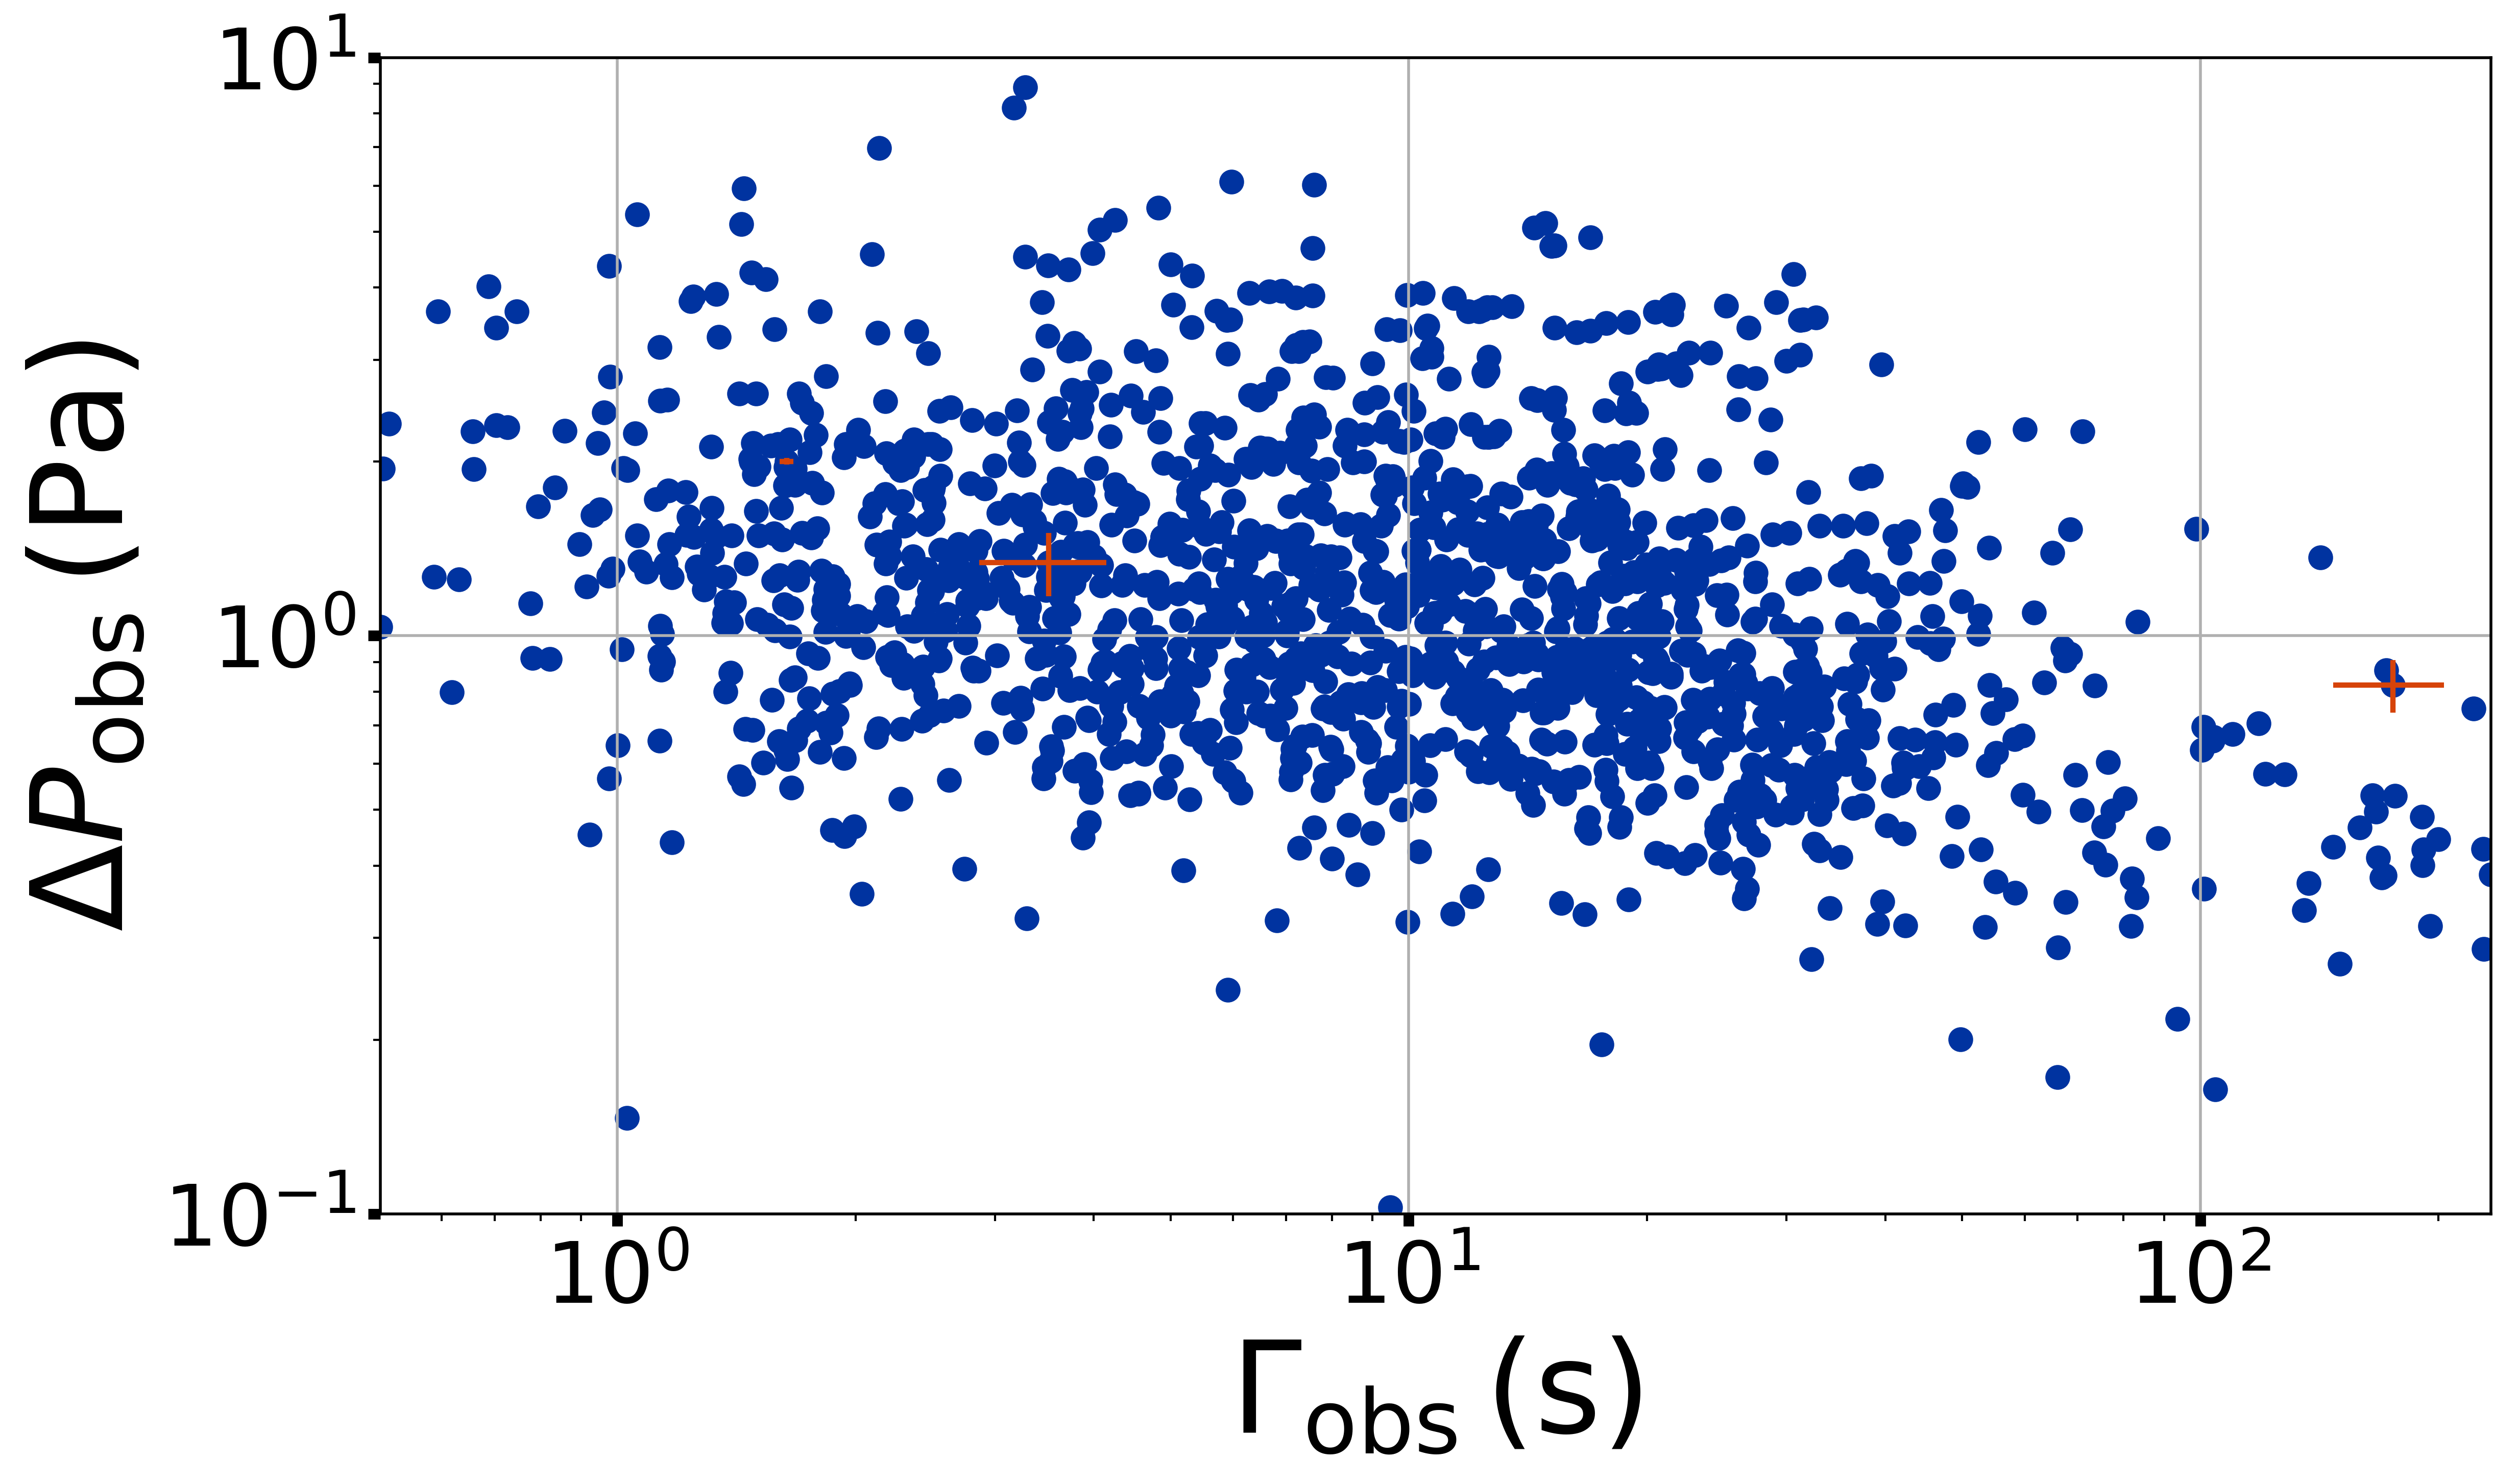
\includegraphics[width=\textwidth]{figures/DeltaPobs_vs_Gammaobs.png}
    \caption{(a) The best-fit $\Delta P_{\rm obs}$- and $\Gamma_{\rm obs}$-values (blue dots). Representative error bars are shown as orange crosses. (b) Cumulative histogram of $\Gamma_{\rm obs}$-values, along with the 50\% quantile value ($\Gamma_{\rm obs} = \left( 9.3 \pm 0.2 \right)\,{\rm s}$) shown by the dashed, orange line. (c) Cumulative histogram of $\Delta P_{\rm obs}$-values, along with the 50\% quantile value ($\Delta P_{\rm obs} = \left( 1.13 \pm 0.03 \right)\,{\rm Pa}$) shown by the dashed, orange line. The dash-dotted green line shows a power-law fit to the histogram, with $N \propto \Delta P_{\rm obs}^{-2.45\pm0.02}$.}
    \label{fig:DeltaPobs_vs_Gammaobs}
\end{figure}

\begin{figure}
    \centering
    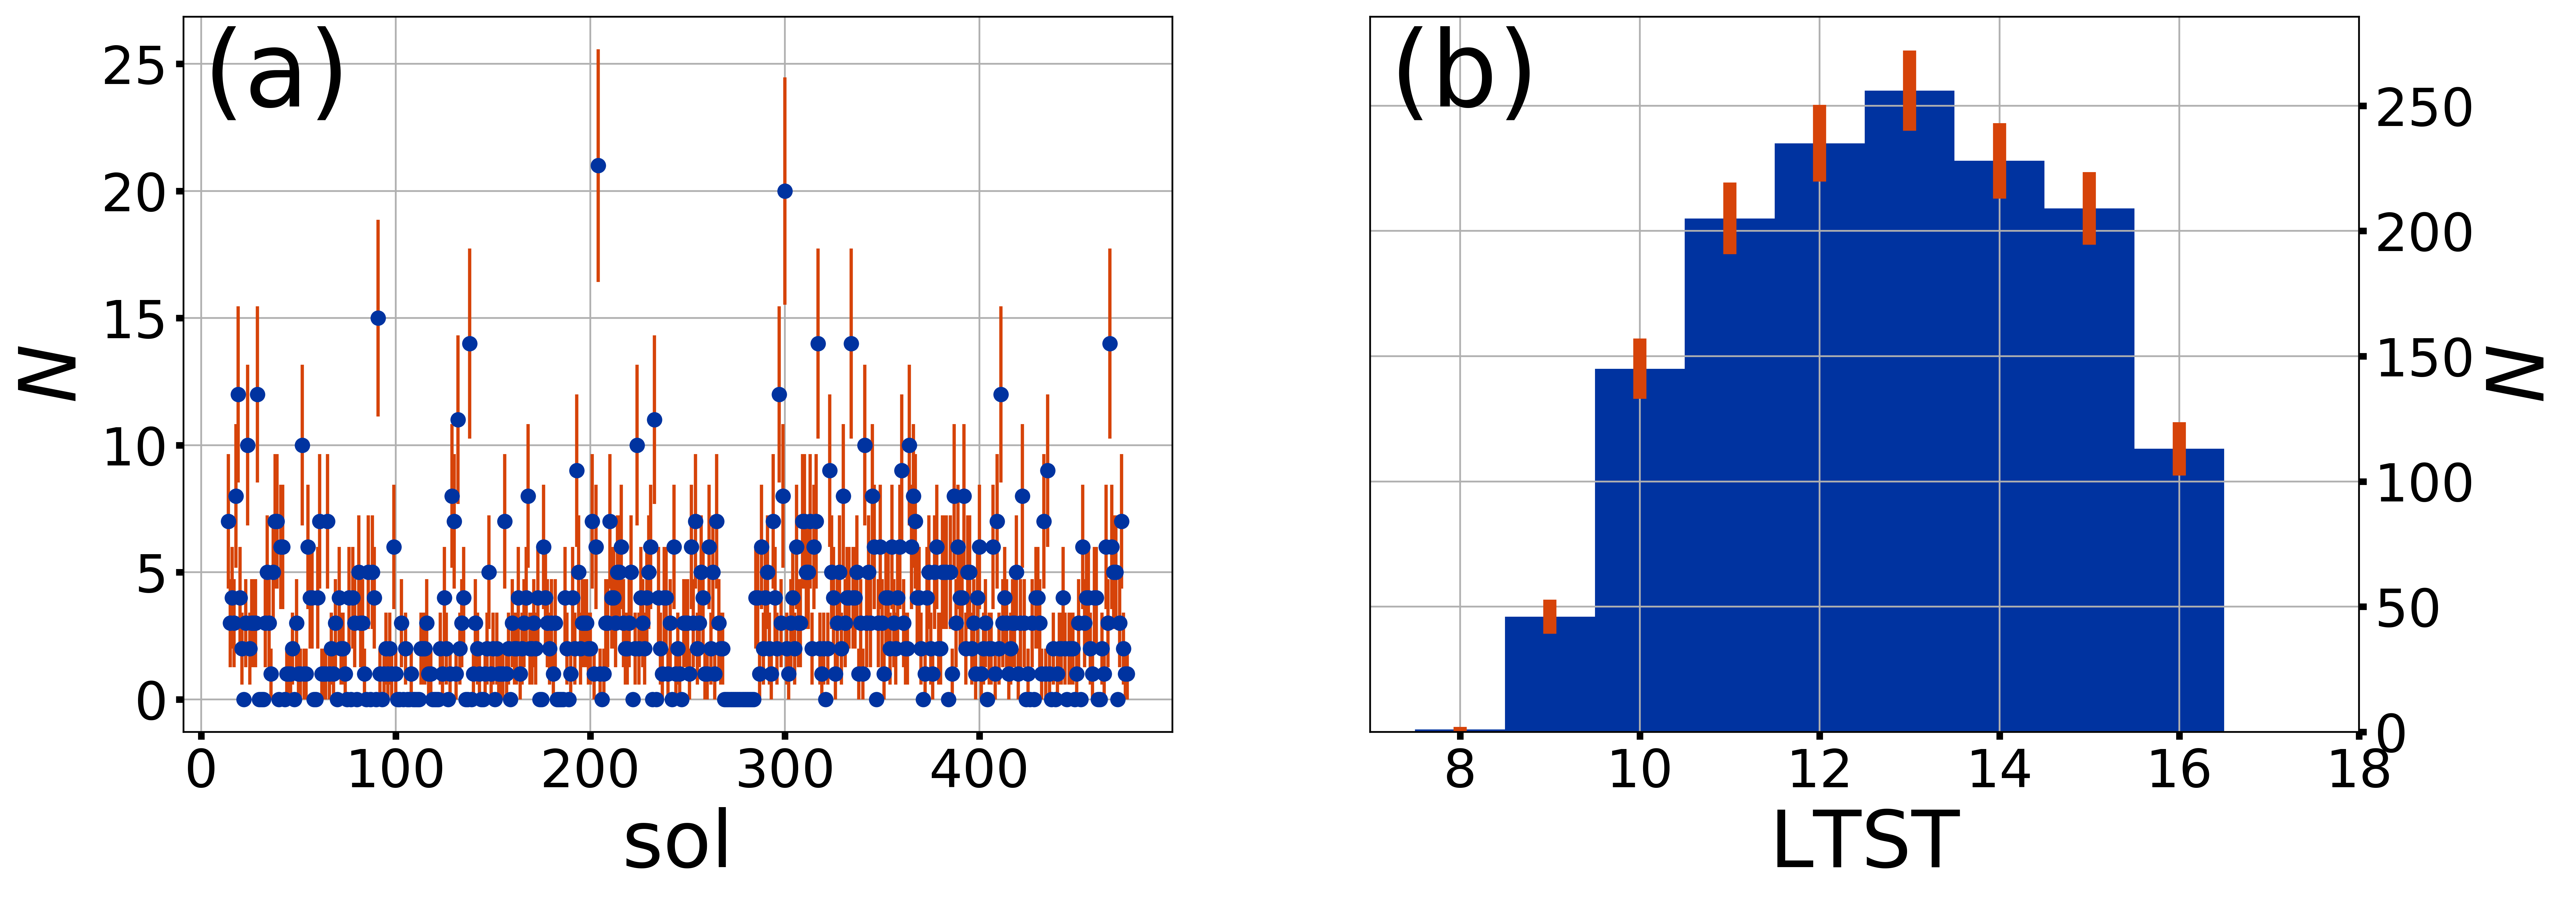
\includegraphics[width=\textwidth]{figures/sol_and_t0_histograms.png}
    \caption{(a) The number of vortices during each sol $N$ (blue dots) along with the values for $L_{\rm s}$ (dashed, grey lines). (Northern spring starts at $L_{\rm s} = 90^\circ$.) The orange histogram shows the number of vortices per sol for bins 35 sols wide. (b) The number of vortices per hour of local true solar time (LTST). Orange lines in both panels show Poisson error bars.}
    \label{fig:sol_and_t0_histograms}
\end{figure}

The vortices also exhibit sol-to-sol and hour-to-hour variation, as illustrated in Figure \ref{fig:sol_and_t0_histograms}. Panel (a) shows that the maximum daily of vortices occurred on sol 204 of the mission, in the middle of northern spring, while the next maximum occurs on sol 300, near the beginning of northern summer. Although \citet{2020arXiv200501134S} used a different procedure, that study found a broadly similar pattern -- a dip in the occurrence rate centered on sol 100, with an increase going into sol 200 and beyond. Regarding the hour-to-hour variations, panel (b) shows that the maximum occurs between 12:00 and 13:00 LTST, with a nearly symmetric decline to either side. For this calculation, we totaled up the number of hours (and fractions thereof) during which pressure time-series were reported and then divided the number of vortices encountered during each of those hours over all sols by that total. These results contrast somewhat with those of \citet{2020arXiv200501134S}, which found a peak in vortex occurrence between 11:00 and 12:00 LTST. 

The $\Gamma_{\rm obs}$- and $\Delta P_{\rm obs}$-values exhibit intriguing trends as well. Figure \ref{fig:Gammaobs_DeltaPobs_vs_TOD_and_sol}(c) shows that, binned by the hour, the median value of $\Gamma_{\rm obs}$ increases from $2$ to $20\,{\rm s}$ from early morning to late afternoon. Figure \ref{fig:Gammaobs_DeltaPobs_vs_TOD_and_sol}(d) shows that median value for $\Delta P_{\rm obs}$ peaks around 12:00 LTST at $\left( 1.3\pm0.05 \right)\,{\rm Pa}$ with minimum values at either end of about $\left( 0.7\pm 0.1 \right)\,{\rm Pa}$ (where the uncertainties come from the error of the median in the corresponding bin). The values binned by sol (Figures \ref{fig:Gammaobs_DeltaPobs_vs_TOD_and_sol}a and b) show no obvious trends. 

\begin{figure}
    \centering
    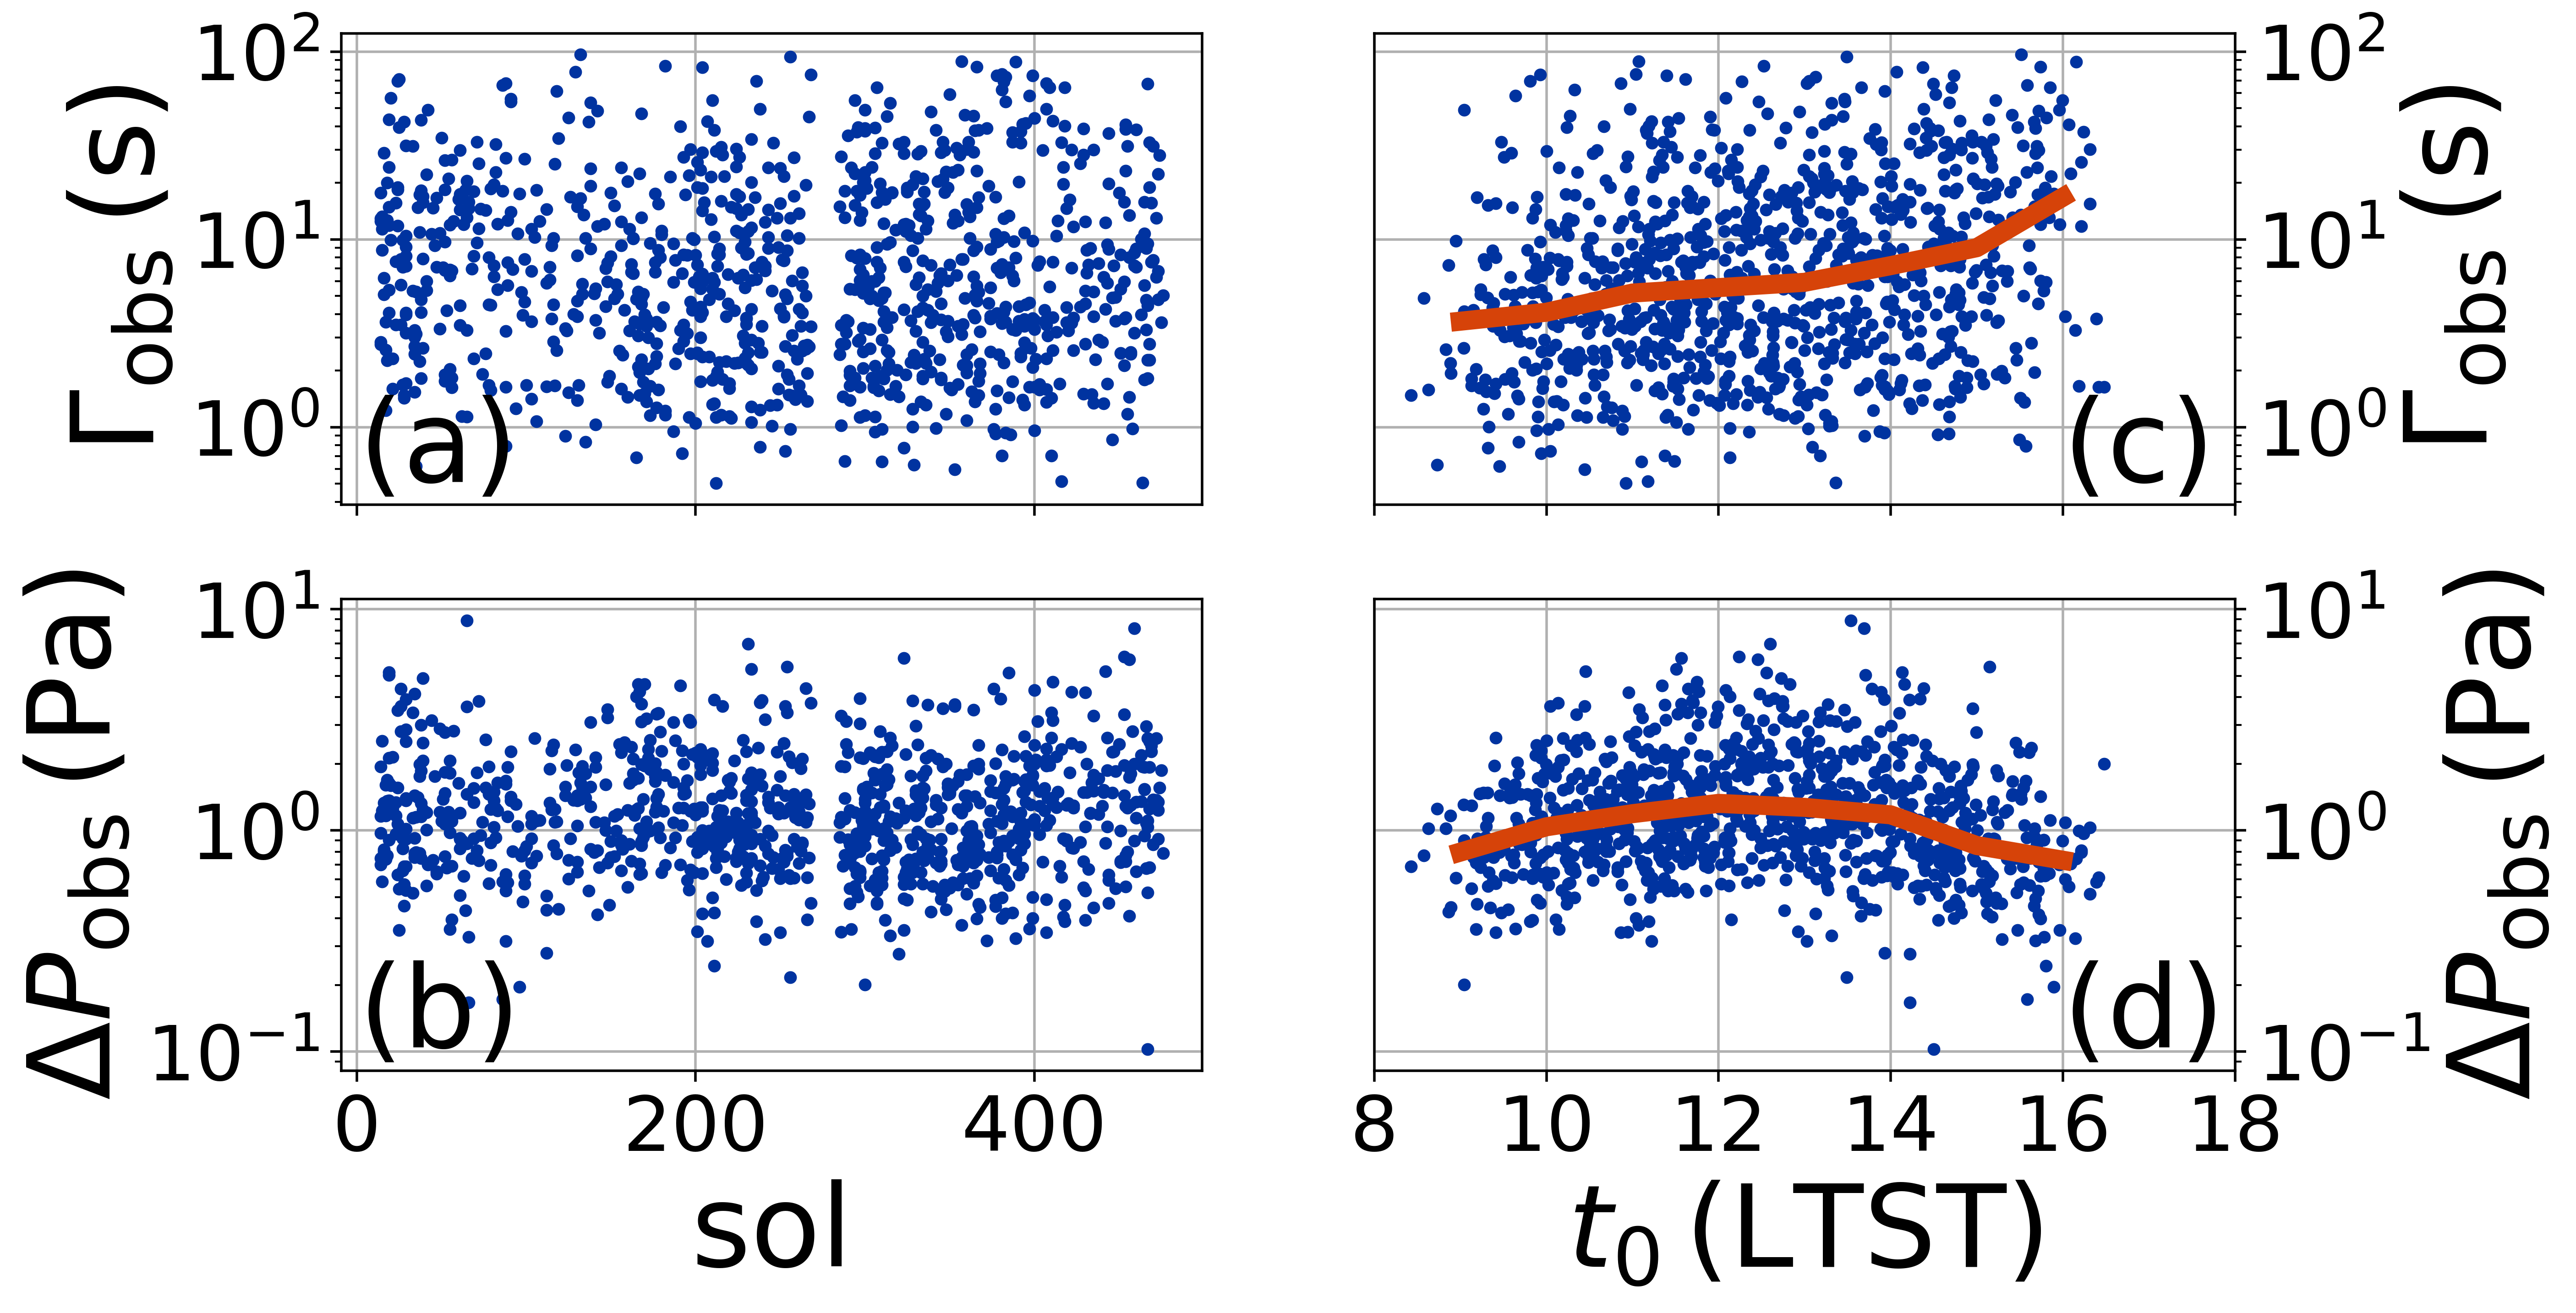
\includegraphics[width=\textwidth]{figures/Gammaobs_DeltaPobs_vs_TOD_and_sol.png}
    \caption{(a)/(b) Distributions of $\Gamma_{\rm obs}$ and $\Delta P_{\rm obs}$ by sol. (c)/(d) Distributions of $\Gamma_{\rm obs}$ and $\Delta P_{\rm obs}$ by time-of-day $t_0$. The orange lines show the distributions binned by hour.}
    \label{fig:Gammaobs_DeltaPobs_vs_TOD_and_sol}
\end{figure}

Presumably, these hour-to-hour trends reflect the influence of variable ambient conditions, but these data alone are not sufficient to judge what influence: the increase in $\Gamma_{\rm obs}$ could result either from intrinsically larger vortices late in the day or lower wind speeds $U$ advecting the same size vortices past the sensor. Fortunately, the TWINS wind speed data can shed light on this issue. Figure \ref{fig:vortices_and_windspeed} shows the three vortices with the largest $\Delta P_{\rm obs}$-values. We estimated the advection speed by taking the median value $U$ between 5- and 3-$\Gamma_{\rm obs}$ before the encounter time $t_0$. This approach returns a wind speed close enough in time to be a plausible estimate of the advection speed but early enough that the vortex did not significantly influence the measurement. 

Figure \ref{fig:U_vs_t0-sol_hist} shows the distribution of advective wind speeds associated with the observed vortices; the maximum, median, and minimum values are $19.1\pm2.3$, $7.6\pm1.0$, and $0.5\pm0.2 \,{\rm m\ s^{-1}}$, respectively. Panel (a) shows a clear decrease in wind speed during the lull in vortex encounters around sol 100 and an increase in wind speeds, along with a widened scatter, during the peak around sol 300. Panel (b) shows a small increase the median advective speed from the early to mid-morning (11:00) and then a steady decline of about 30\% thereafter. This decline in advection speed correlates very closely with the increase in $\Gamma_{\rm obs}$ from 11:00 to 16:00 LTST. Assuming uniformly distributed random encounter distances $b$, we expect the vortex duration to scale inversely with advection speed. Consequently, the increase in $\Gamma_{\rm obs}$ seen in Figure \ref{fig:Gammaobs_DeltaPobs_vs_TOD_and_sol}(c) seems likely to result from the decrease in advection speed, not from a systematic increase in vortex diameter. Indeed, the decline in $\Delta P_{\rm obs}$ seen in the afternoon comports with this result \citep{2020Icar..33813523J}.

% Figure \ref{fig:Dobs_vs_Gammaobs-DeltaPobs_hist} shows the distribution of $D_{\rm obs}$-values against $\Gamma_{\rm obs}$ and $\Delta P_{\rm obs}$, as well as a cumulative histogram. The maximum, minimum, and median values are $1100 \pm 240$, $75 \pm 21$, and $4 \pm 1 \,{\rm m}$, respectively. Not surprisingly, the $D_{\rm obs}$-values correlate positively with $\Gamma_{\rm obs}$ with scatter resulting from the relatively narrow range of advective wind speeds. 
% On the other hand, $D_{\rm obs}$ seems negatively correlated with $P_{\rm obs}$, and a power-law fit using the Levenberg-Marquardt algorithm \citep{Press2007} gives $D_{\rm obs} \propto \Delta P_{\rm obs}^{-0.42\pm0.04}$, where uncertainties come from the covariance matrix. As explained in \citet{2018Icar..299..166J}, for a vortex encounter with any miss distance $b$, we expect $\Delta P_{\rm obs}$ and $D_{\rm obs}$ are related to the vortex's central pressure excursion $\Delta P_{\rm act}$ and diameter $D_{\rm act}$ as $\Delta P_{\rm obs} D_{\rm obs}^2 = \Delta P_{\rm act} D_{\rm act}^2$. Figure \ref{fig:Dobs_vs_Gammaobs-DeltaPobs_hist}(b) could be interpreted, then, as encounters with vortices at a variety of miss distances but all with the same $\Delta P_{\rm act}$- and $D_{\rm act}$-values (the exponent $0.4\pm0.04$ diverges from 0.5 by less than $3\sigma$). However, such a result is totally unexpected as dust devil diameters are known to span a wide range and would be inconsistent with a variety of studies \citep[cf.][]{2016SSRv..203..277L}. Instead, this result probably only indicates that the range of miss distances plays an important role in setting the observed distribution. 

\begin{figure}
    \centering
    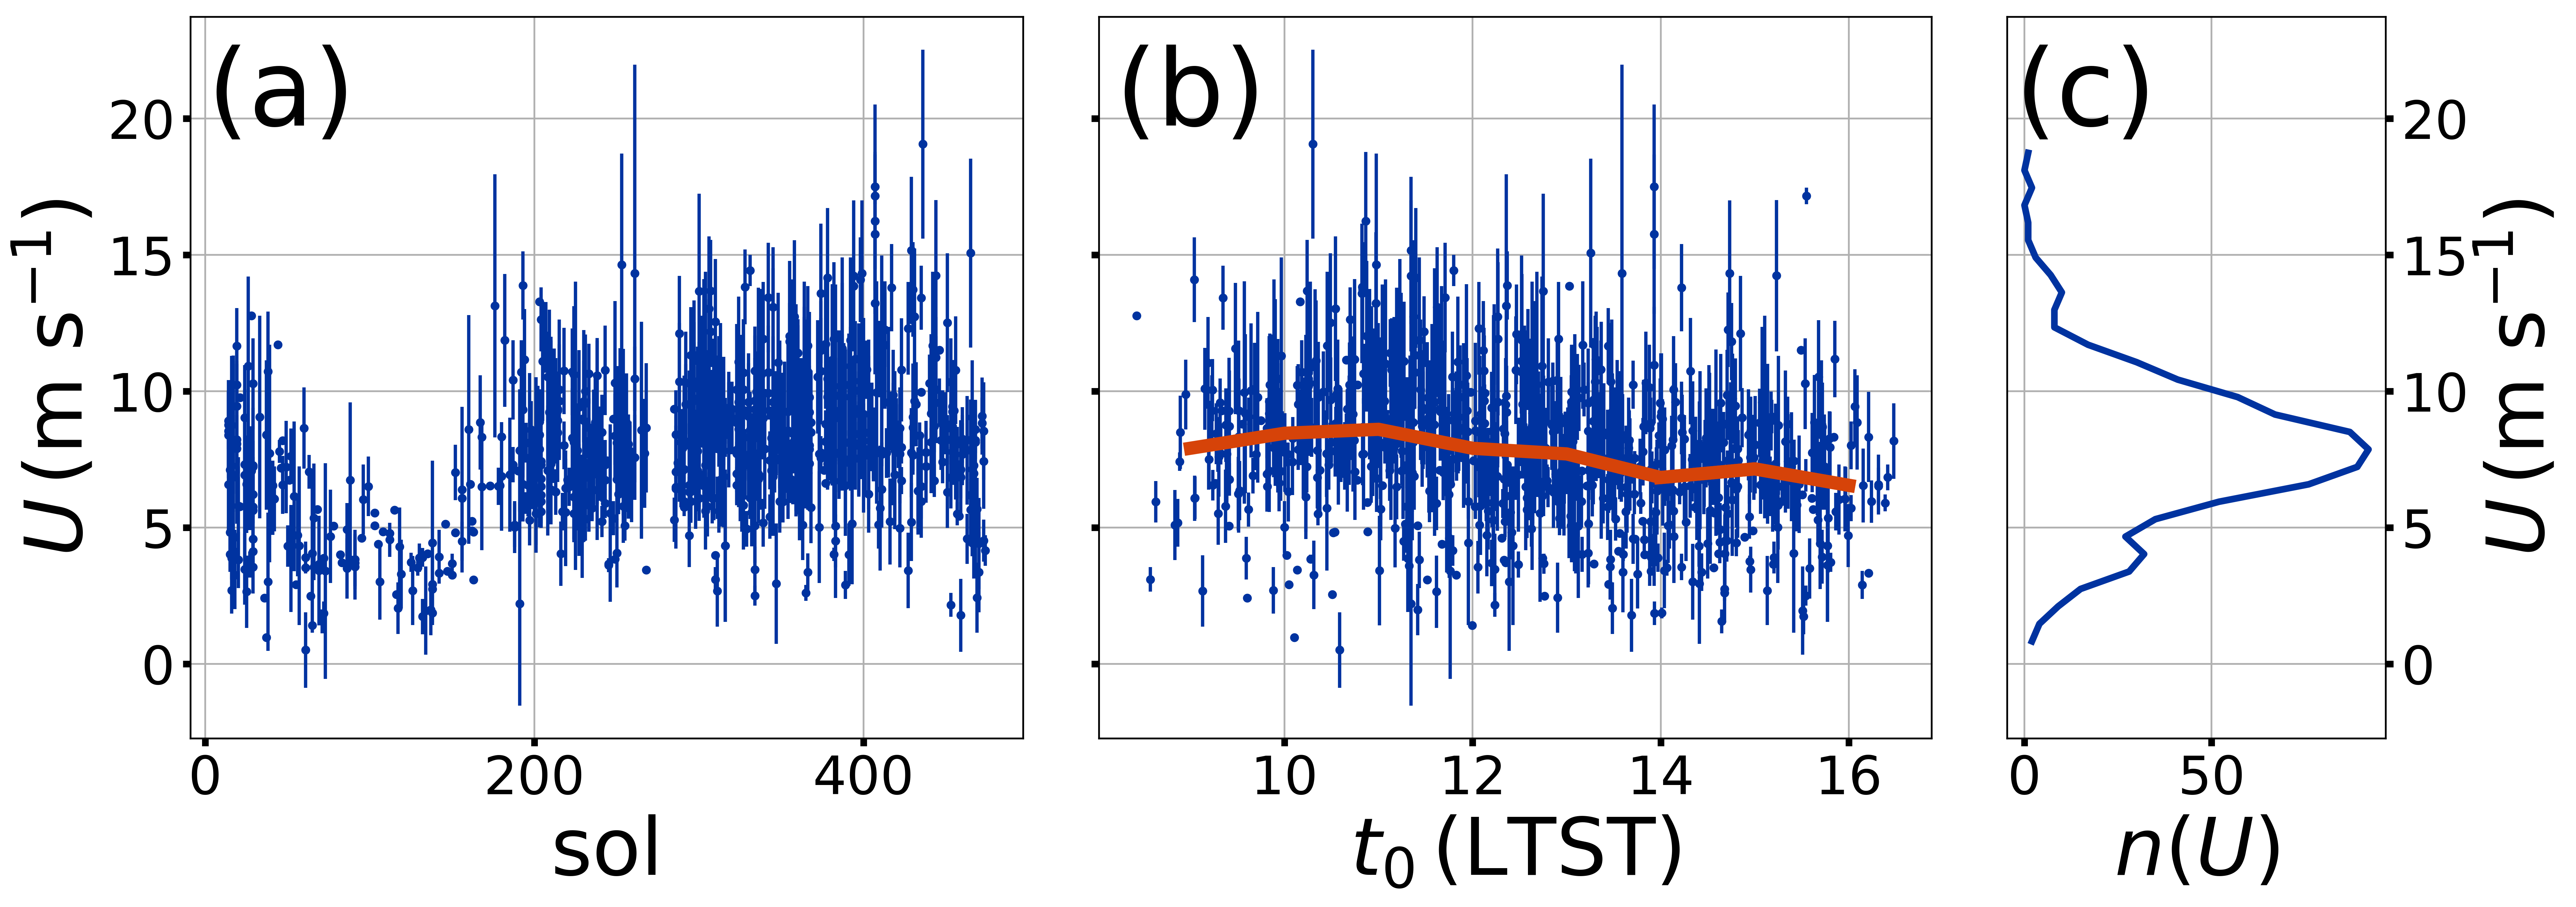
\includegraphics[width=\textwidth]{figures/U_vs_t0-sol_hist.png}
    \caption{Distribution of vortex-associated wind speeds $U$ as a function of time of day (a) and mission sol (b). Panel (c) shows a differential (as opposed to cumulative) histogram of $U$-values.}
    \label{fig:U_vs_t0-sol_hist}
\end{figure}

% \begin{figure}
%     \centering
%     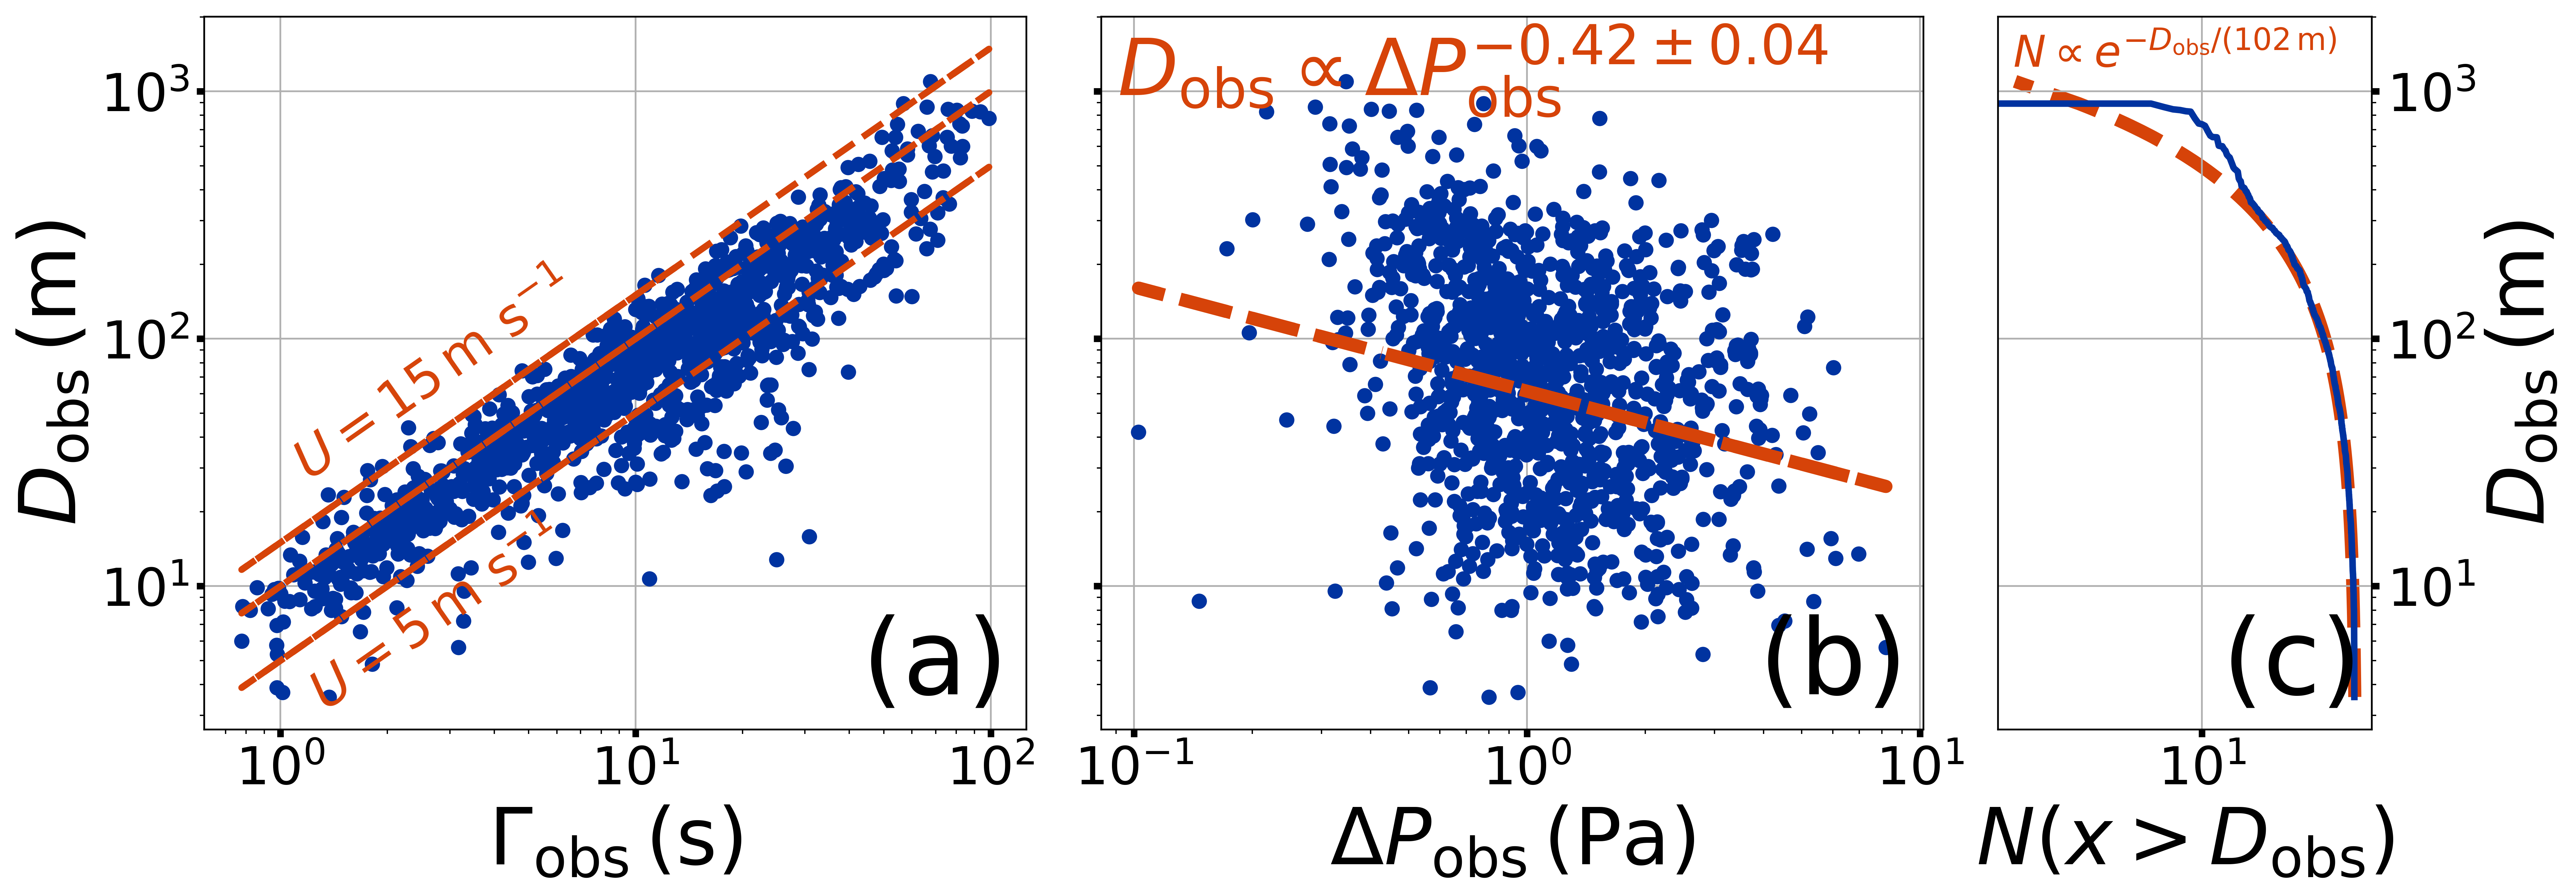
\includegraphics[width=\textwidth]{figures/Dobs_vs_Gammaobs-DeltaPobs_hist.png}
%     \caption{(a) Distribution of inferred vortex diameter $D_{\rm obs}$ from the observed $\Gamma_{\rm obs}$ (blue dots). Uncertainties on $D_{\rm obs}$ suppressed for clarity but are typically about $15\,{\rm m}$ or 10\% of $D_{\rm obs}$. Orange, dashed lines show a range of wind speeds $U$ -- $15$, $10$, and $5\,{\rm m\ s^{-1}}$ from top to bottom. (b) $D_{\rm obs}$ vs. each vortex's $\Delta P_{\rm obs}$. (c) Cumulative histogram of $D_{\rm obs}$, $N(x > D_{\rm obs})$ (blue curve), along with an exponential fit of the form $N \propto e^{D_{\rm obs}/D_0}$ with $D_0 = \left( 130.1 \pm 0.2 \right)\,{\rm m}$.}
%     \label{fig:Dobs_vs_Gammaobs-DeltaPobs_hist}
% \end{figure}

\citet{2018Icar..299..166J}, \citet{2019Icar..317..209K}, and \citet{2020Icar..33513389K} developed approaches to de-bias the observed population of vortices and work out the underlying distribution of $\Delta P_{\rm act}$- and $D_{\rm act}$-values. However, they rely on plausible but untested assumptions about encounter statistics. Fortunately, as discussed in Section \ref{sec:Pressure and Wind Models} and Appendix \ref{sec:Inferring Encounter Geometries from the Pressure and Velocity Profiles}, we can use the observed vortex wind and pressure excursions themselves to work out the intrinsic parameters. The best-fit full and simple wind profile models are illustrated for the three representative vortex encounters in Figure \ref{fig:vortices_and_windspeed}. Figure \ref{fig:Dact_vs_Pact} shows the inferred $P_{\rm act}$- and $D_{\rm act}$-values for the \agreeablevortices\ encounters for which the inferred $P_{\rm act}$ and $D_{\rm act}$ from both the full and simple wind profiles agree to within 25\%. (For many other encounters, the two profiles return significantly different values, or the Levenberg-Marquardt fitting scheme fails to converge on a value for the full profile.) We also require that the inferred $|b|/D_{\rm act} < 10$ and that observed wind speed excursion $V_{\rm obs}$ is more than 3-$\sigma$ different from the pre-encounter ambient wind speed $U_1$. This criterion ensures that we detected a true vortex encounter, rather than simply a pressure excursion. (For \vorticeswithnowinds\ encounters, we found the simple and full wind profile fits agreed but gave $V_{\rm obs}$ statistically consistent with $U_1$.) For the uncertainties on $P_{\rm act}$ and $P_{\rm act}$, we take half the difference between the values returned using the simple and full wind profile models.

\begin{figure}
    \centering
    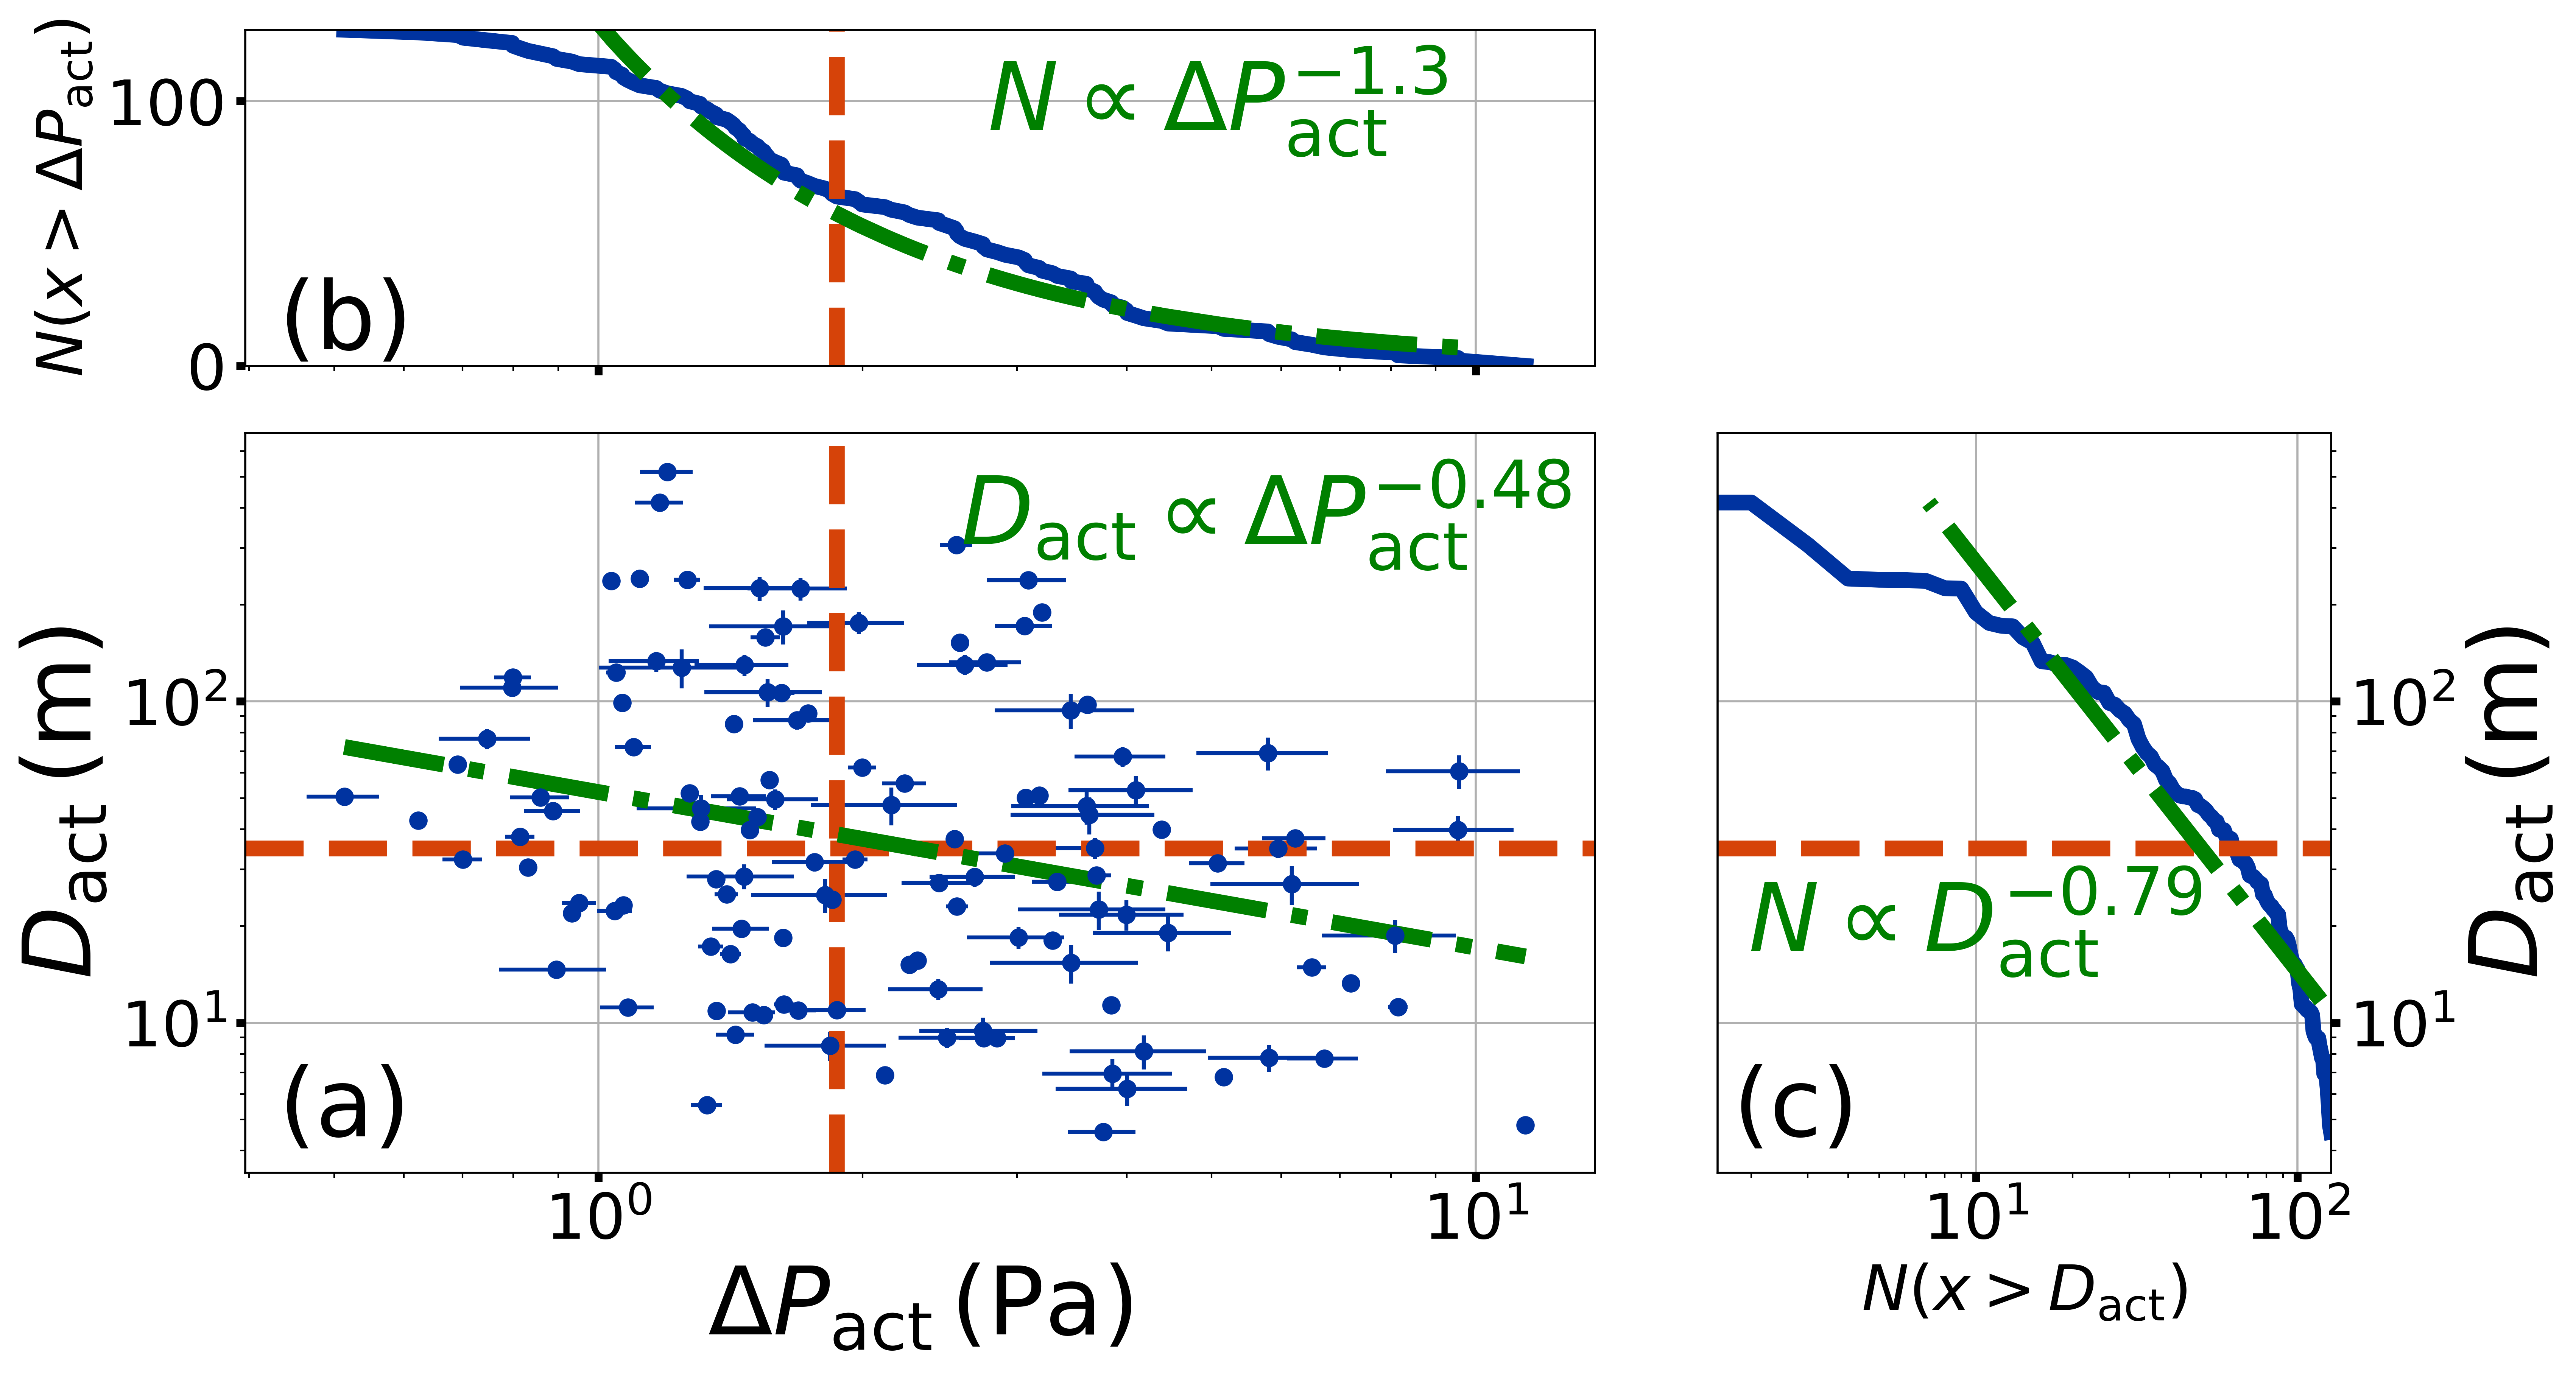
\includegraphics[width=\textwidth]{figures/Dact_vs_Pact.png}
    \caption{(a) Distribution of estimated actual vortex diameters $D_{\rm act}$ vs. the pressure excursions $P_{\rm act}$ (blue dots) with uncertainties, along with a power-law fit (dashed, orange line). (b) Cumulative histogram of $P_{\rm act}$-values. (c) Cumulative histogram of $D_{\rm act}$-values.}
    \label{fig:Dact_vs_Pact}
\end{figure}

Although difficulties robustly modeling the wind profiles makes Figure \ref{fig:Dact_vs_Pact} more sparse than Figure \ref{fig:DeltaPobs_vs_Gammaobs}, interesting patterns still emerge. 

\section{Discussion and Conclusions}
\label{sec:Discussion and Conclusions}

What do these choices mean about our ability to accurately recover the vortex population? The answer will depend, in part, on the properties of the vortex population itself, and \citet{2018Icar..299..166J} discuss many of the relevant details. In brief, in order for our scheme to detect a vortex with given $\Delta P_{\rm act}$- and $D_{\rm act}$-values, it must register in the time-series with 
\begin{equation}
    \Delta P_{\rm obs} &=& \frac{\Delta P_{\rm act}}{1 + \left(2b/D_{\rm act}\right)^2} &>& P_{\rm min},\label{eqn:Pobs} 
\end{equation}
where $b$ is the closest approach distance between the sensor and the vortex center and $P_{\rm min}$ is the minimum pressure excursion detectable. Figure \ref{fig:vortex_recovery} shows that, for $\log \Gamma/\Gamma_{\rm obs} < 0.5$ at least, $\Delta P_{\rm obs} \gtrsim 0.3 \sigma_P$. In other words, for the typical APSS pressure time-series with $\sigma_P \lesssim 1\,{\rm Pa}$ (Figure \ref{fig:Pobsprime-sigmaP_vs_W}(b)), we could, in principle, recover vortices with $\Delta P_{\rm obs} \approx 0.3\,{\rm Pa}$. Since the sampling rate for the APSS barometer (1 Hz) means we cannot detect devils with durations $\Gamma_{\rm obs} < 1\,{\rm s}$, we take $\Gamma = 1\,{\rm s}$ for our matched filter, meaning the limit imposed by $\Gamma/\Gamma_{\rm obs}$ is easily dealt with.

With these choices, the maximum distance out to which we could detect a vortex is given by
\begin{equation}
    b_{\rm max} = \left( \frac{D_{\rm act}}{2} \right) \sqrt{ \frac{\Delta P_{\rm act}}{\Delta P_{\rm min}} - 1 }. \label{eqn:bmax}
\end{equation} 

As discussed in Section \ref{sec:Introduction}, the quantity of meteorological interest is $N$, the number of vortices per unit area, which can be estimated from the total number of vortex detections, $k$, via
\begin{equation}
    k = 2 N U T b_{\rm max} = N U T D_{\rm act} \sqrt{ \frac{\Delta P_{\rm act}}{\Delta P_{\rm min}} - 1 }, \label{eqn:number_of_encounters}
\end{equation}
where $T$ is the total duration of the survey (which may consist of multiple observational sequences spread over many sols). (If $N$ and $U$ evolve with time (as they usually do), this estimate can be converted into an integral over time.) A reasonable assumption is that vortex encounters represent a Poisson process \citep[cf.][]{Press2007}, and so we can estimate the uncertainty on $k$ as $\sigma_k = \sqrt{k}$ and therefrom the uncertainty $\sigma_N$ via
\begin{equation}
    \frac{\sigma_N}{N} = \frac{\sigma_k}{k} = k^{-1/2} = \left ( N U T D_{\rm act} \right)^{-1/2} \left( \frac{\Delta P_{\rm act}}{\Delta P_{\rm min}} - 1 \right)^{-1/4}.
    \label{eqn:sigma_N}
\end{equation}

\section{Camera Model}
To begin with, we outline the very basic characteristics of our model camera. By design, the considerations here are simplistic and general, rendering them applicable to a wide range of imaging systems. Consider a camera angled to have a clear view of the horizon and with a horizontal field-of-view $\Delta_{\rm FOV}$ centered on azimuth $\lambda$ and an angular resolution $\alpha$ measured in angle per pixel (Figure \ref{fig:Awedge}). Consider also a dust devil with a fixed diameter $D$, height $H$, and a sufficient contrast against the image background that it can be detected. Such a dust devil could be resolved at a distance from the camera $r_{\rm max} = D/\alpha$. For example, to resolve a dust devil with $D = 10\,{\rm m}$ with three pixels across, if $\alpha = 0.3\,{\rm mrad\ pix^{-1}} \times 3\,{\rm pix} \approx 1\,{\rm mrad}$ (similar to the Mars 2020 Mastcam-Z - \citealp{2017E&SS....4..396B}), $r_{\rm max} \approx 10\,{\rm km}$.

\begin{figure}
    \centering
    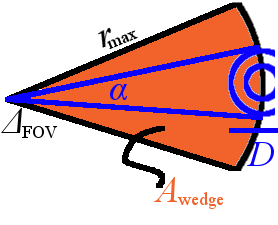
\includegraphics[width=0.5\textwidth]{figures/Awedge.jpg}
    \caption{Observational geometry. The camera has a field-of-view is $\Delta_{\rm FOV}$ and an angular resolution $\alpha$ which allows it to resolve dust devils of diameter $D$ out to a radial distance $r_{\rm max}$. The area surveyed is $A_{\rm wedge}$.}
    \label{fig:Awedge}
\end{figure}

In principle, the camera could detect this dust devil if it traversed the pie-wedge of terrain centered on $\lambda$ and having an area 
\begin{equation}
    A_{\rm wedge} = \frac{\Delta_{\rm FOV} r_{\rm max}^2}{2} = \frac{\Delta_{\rm FOV}D^2}{2 \alpha^2}.
    \label{eqn:A_wedge}
\end{equation}
Taking the same $D$ and $\alpha$-values as above, along with $\Delta_{\rm FOV} = \pi/2\,{\rm rad}$ gives $A_{\rm wedge} \sim 100\,{\rm km^2}$. If dust devils traveled very slowly (or not at all) from their origin point, then the survey would only include devils that appeared within this wedge. However, as pointed out in \citet{2014JAtS...71.4461L}, advection of dust devils through a survey site increases the effective area surveyed. 

Consider a fixed, unidirectional wind of speed $U$ crossing perpendicularly through the pie-wedge. If the dust devil under consideration has a lifetime $\tau$, then it will travel a distance $L = \tau U$ before dissipating. Thus, the wind field can advect dust devils into the camera's field-of-view acting as a conveyor belt with area
\begin{equation}
    A_{\rm adv} = r_{\rm max} L = \frac{D U \tau}{\alpha}.
    \label{eqn:A_adv}
\end{equation}
Again, typical values $D \sim 10\,{\rm m}$, $U \sim 10\,{\rm m\ s^{-1}}$, $\tau \sim 100\,{\rm s}$, and $\alpha \sim 1\,{\rm mrad}$ gives $A_{\rm adv} \sim 10\,{\rm km^2} \ll A_{\rm wedge}$. Although both areas contribute, we neglect $A_{\rm adv}$ compared to $A_{\rm wedge}$, and we use this estimate for the area surveyed $A_{\rm survey} \approx A_{\rm wedge}$ to determine how the inferred population of dust devils depends on the survey parameters.

\section{Imaging Surveys for Distant Dust Devils}
First, we consider the accuracy with which we could infer the occurrence rate of dust devils detected very distant from the instrument suite and that register only on the camera instrument. We can relate the areal density $N$ (dust devils per unit area) for a certain period of interest from the total number of dust devils observed in a single image $k$:
\begin{equation}
   N = \frac{k}{A_{\rm survey}} = \left( \frac{2 \alpha^2}{\Delta_{\rm FOV} D^2} \right)\ k.
    \label{eqn:areal_occurrence}
\end{equation}

If we assume that dust devil occurrence is a Poisson process, then we can estimate the standard deviation or uncertainty on $k$ as $\sigma_k = \sqrt{k}$ and the uncertainty $\sigma_N$ on our estimate of $N$ via
\begin{equation}
    \frac{\sigma_N}{N} = \frac{\sigma_k}{k} = k^{-1/2} = \sqrt{2} N^{-1/2} D^{-1}\ \Delta_{\rm FOV}^{-1/2} \alpha.
    \label{eqn:sigma_N}
\end{equation}

\begin{figure}
    \centering
    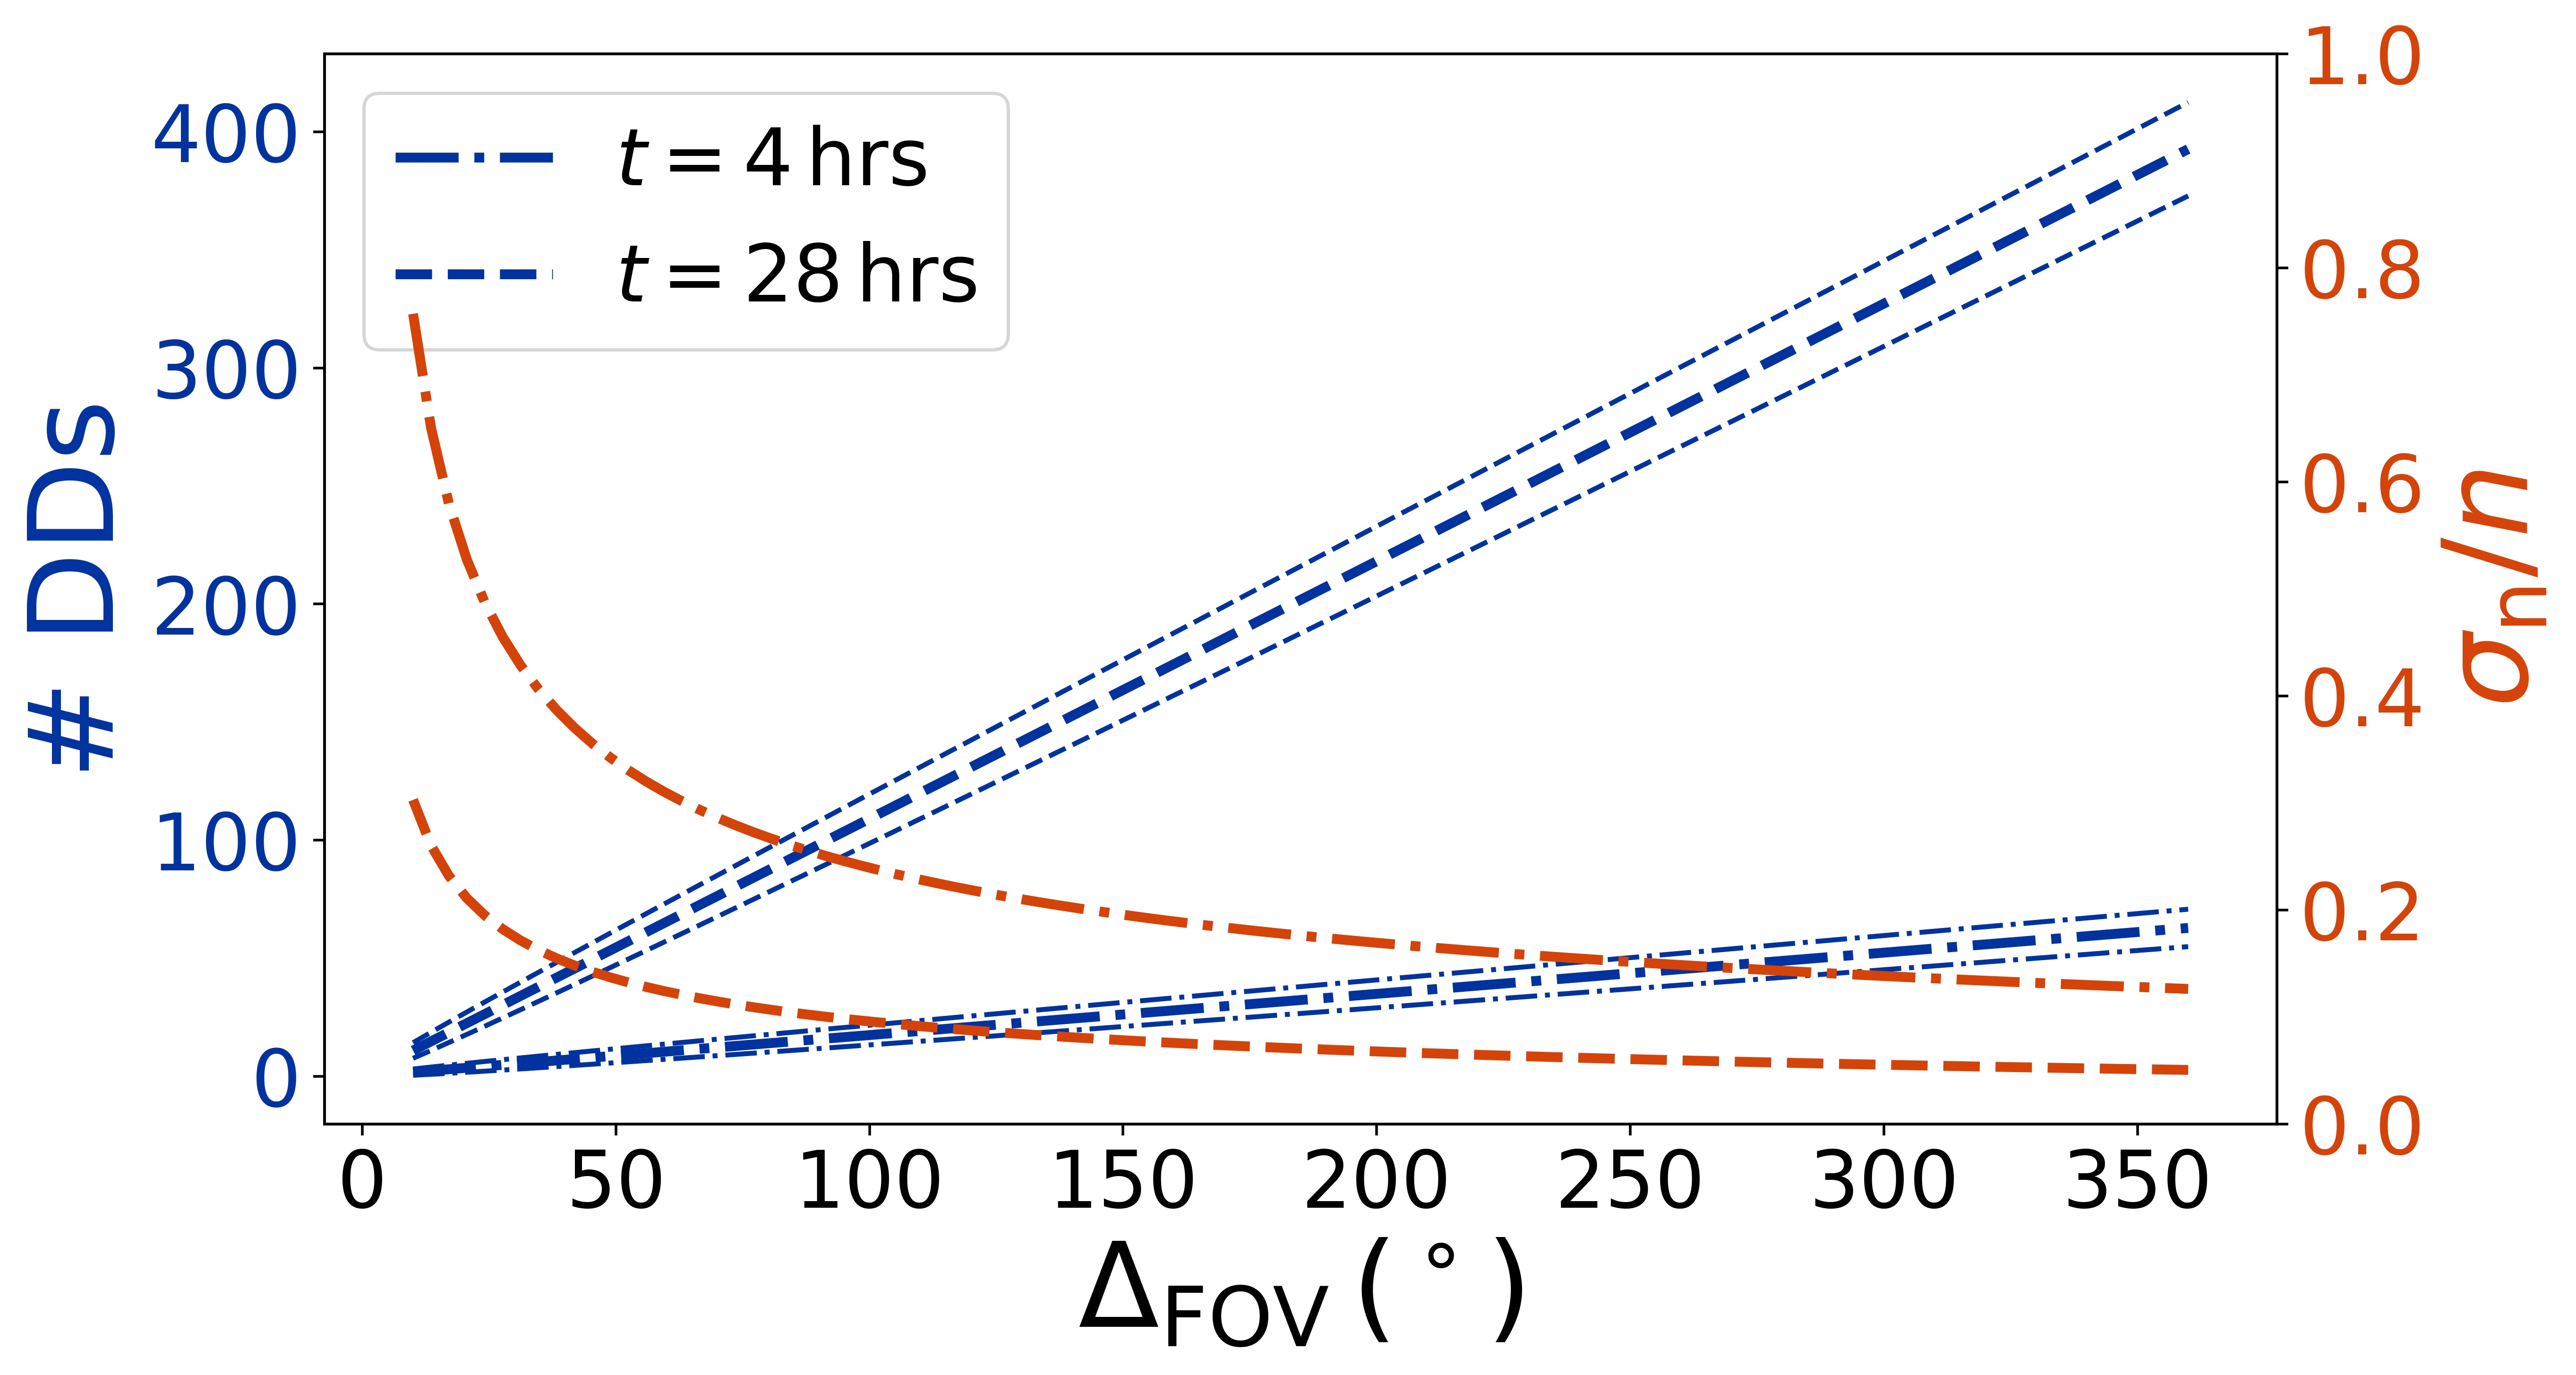
\includegraphics[width=\textwidth]{figures/DDs_vs_Delta.jpg}
    \caption{The expected range of dust devils recovered in an image as a function of field-of-view $\Delta_{\rm FOV}$ (filled blue region). The survey precision, $\sigma_N/N$ is shown as a dash-dot, orange line. The calculation here assumes $N = 0.03\,{\rm km^{-2}}$, $D = 10\,{\rm m}$, and $\alpha = 1\,{\rm mrad}$.}
    \label{fig:DDs_vs_Delta}
\end{figure}

% Usually, we would design our survey so that we achieve a sufficiently precise estimate for the quantity of physical significance $N$. In other words, we would require $\sigma_N/N < T$, some threshold. We can see that Equation \ref{eqn:sigma_N} provides the specific requirements to achieve the desired threshold. For instance, we can take some typical values from \citet{2006JGRE..11112S09G} and estimate what minimum angular resolution is required of our camera to achieve $T = 0.1$:
% \begin{equation}
%     \alpha < 2^{-1/2} T \left( n t \right)^{1/2} D\ \Delta_{\rm FOV}^{1/2} = 2^{-1/2} \left( 0.1 \right) \big[ \left( 0.05\,{\rm km^{-2}\ hr^{-1}} \right) \left( 1\,{\rm hr} \right) \big]^{1/2} \left( 10\,{\rm m} \right) \left( \pi/2\,{\rm rad} \right)^{1/2} \approx 0.2\,{\rm mrad}.
%     \label{eqn:alpha_example}
% \end{equation}
% Such an angular resolution is about ten times better than is usually achieved -- the MER Hazcams used for the survey in \citet{2006JGRE..11112S09G} had a resolution of $2\,{\rm mrad/pix}$ \citep{2003JGRE..108.8071M}.

Another application of Equation \ref{eqn:sigma_N} might instead involve assuming requiring a minimum survey accuracy $T = \sigma_N/N$ and asking, for a given camera field-of-view, what angular resolution is required. Figure \ref{fig:alpha_vs_Delta} shows the result: an accuracy of $T = 50\%$ can be achieved with $\Delta_{\rm FOV} = 150^\circ$ and a modest $\alpha = 1\,{\rm mrad}$ (i.e., resolving a dust devil with pixels across if the pixels each have a resolution of $0.3\,{\rm mrad\, pix^{-1}}$), again for $N = 0.03\,{\rm km^{-2}}$.

\begin{figure}
    \centering
    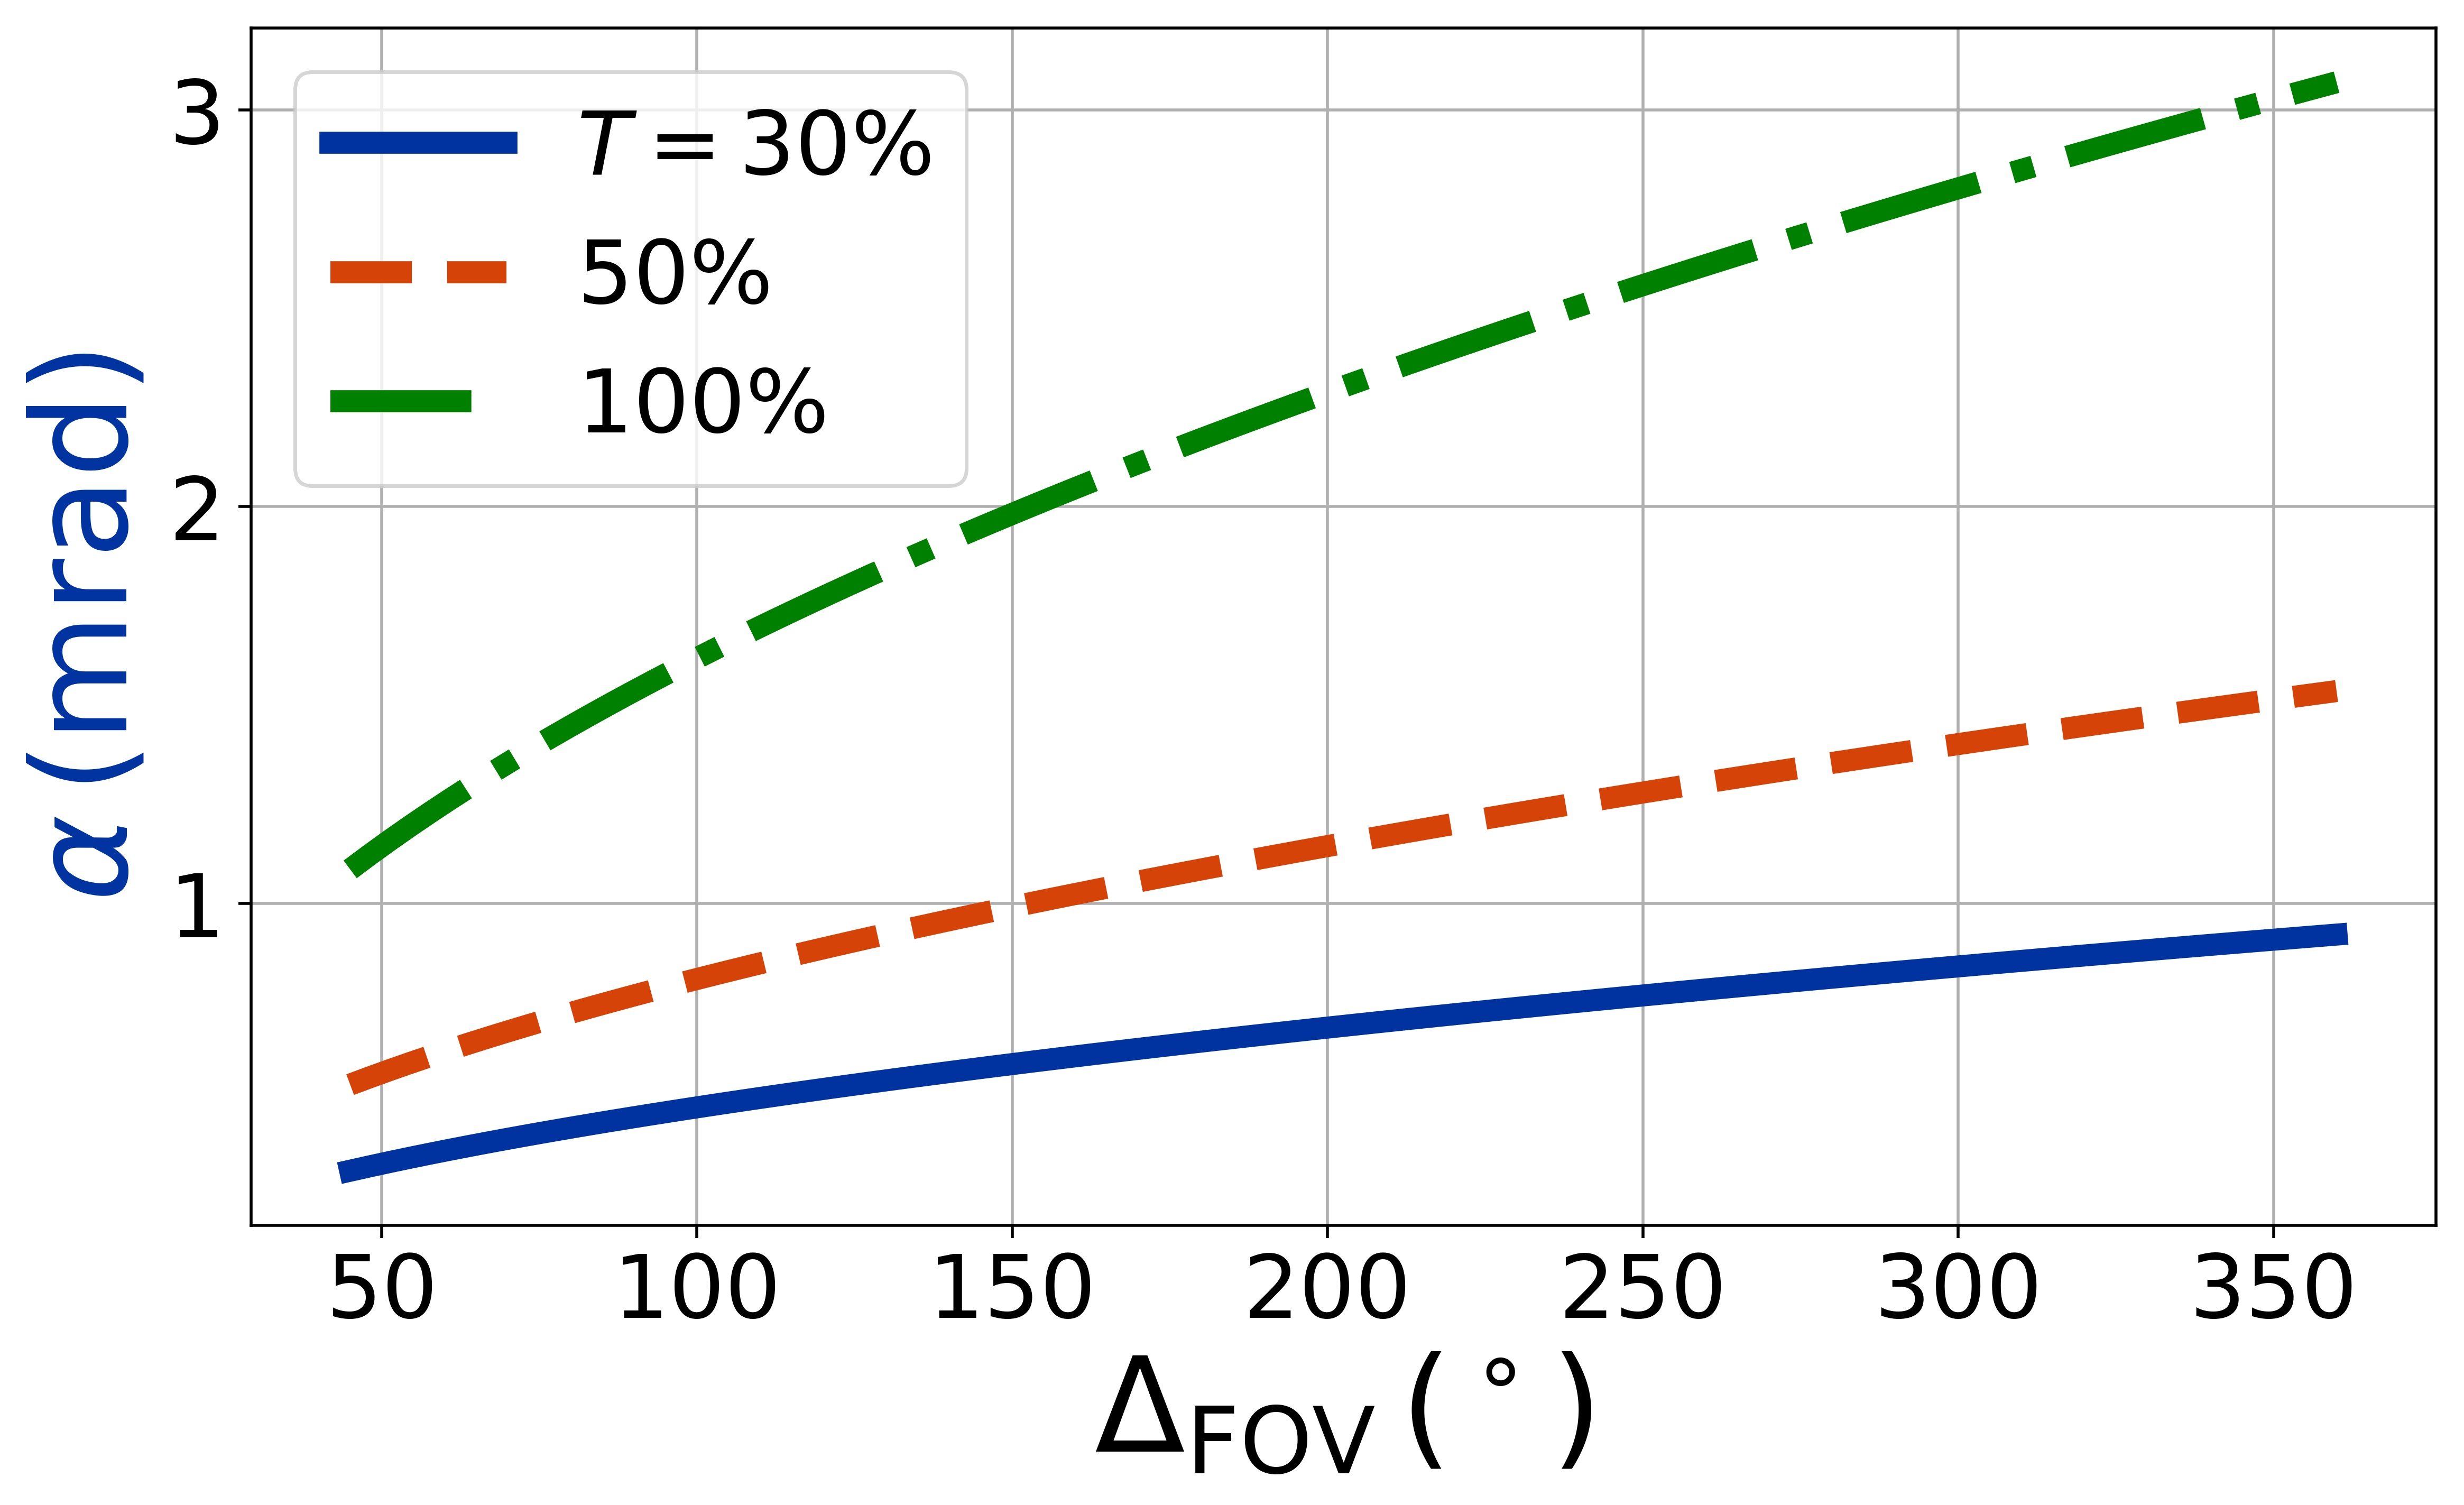
\includegraphics[width=\textwidth]{figures/alpha_vs_Delta.jpg}
    \caption{The $\Delta_{\rm FOV}$-$\alpha$ combinations required to achieve a desired survey accuracy $T = \sigma_N/N$. The calculation here assumes $N = 0.03\,{\rm km^{-2}}$ and $D = 10\,{\rm m}$.}
    \label{fig:alpha_vs_Delta}
\end{figure}

However, dust devils are usually active only for a few hours during each day (or sol on Mars) -- \citet{2006JGRE..11112S09G} found negligible activity before 9 a.m. LTST or after 5 p.m. LTST. Moreover, the occurrence rate itself seemed to evolve over the course of the active phase, increasing from $0.005\,{\rm km^{-2}\ hr^{-1}}$ early in the morning to  $0.05\,{\rm km^{-2}\ hr^{-1}}$ around noon. This mid-day peak agrees with meteorological predictions that dust devil activity should increase as the planetary boundary layer deepens with increasing surface heating \citep{doi:10.1029/2010RG000351}. Accurately estimating the occurrence rate requires a survey duration not longer than the timescale of variability, i.e., about an hour. Therefore, the 25-hours of survey required to recover $n = 0.05\,{\rm km^{-2}\ hr^{-1}}$ to 10\% accuracy would have to be spread into 1-hour surveys around noon spanning 25 sols. (And, of course, smaller occurrence rates would require additional time.) 

Similarly, \citet{2006JGRE..11112S09G} reported an occurrence rate that varied with season and $L_{\rm S}$. Assuming sufficient daily coverage to accurately capture the daily occurrence rate (i.e., a large enough value for $n t$), we can ask what $\Delta_{\rm FOV}$ might be required to recover the seasonal variability by looking at the expected variation in $n t$. From its peak in spring to the peak in summer, $n t$ dropped from $0.11\,{\rm km^{-2}}$ to $0.05\,{\rm km^{-2}}$, which would require a precision $\sigma_n/n \sim 0.5$. Solving Equation \ref{eqn:sigma_n} gives $\Delta_{\rm FOV} \approx 65^\circ$. Considering instead the maximum $\Delta_{\rm FOV} = 360^\circ$ and an areal occurrence $nt = 0.11\,{\rm km^{-2}}$ suggests we could recover dozens of 10-m wide dust devils. 

Importantly, all these calculations up till now have assumed a single dust devil diameter, $D$. In fact, dust devils span a range of diameters - \citet{2006JGRE..11112S09G} reported values between 2 and $276\,{\rm m}$, while orbital studies have reported devils hundreds of meters across \citep{2008Icar..197...39S}. However, the distribution of diameters appears to follow a steep power law, with an exponent between 1 and 2 \citep{2016SSRv..203..277L}. Consequently, the majority of devils reported in \citet{2006JGRE..11112S09G} lay between 10 and $20\,{\rm m}$, and so $n$ is dominated by devils in this range and the calculations presented so far may be considered reasonably representative. In addition, for a given angular resolution, larger dust devils can be recovered from farther away, an observational bias that has been previously pointed out \citep{2012Icar..219..556K, 2013Icar..226..964L}.

On the other hand, given that larger dust devils are less common, they may be intrinsically less likely to be recovered. Equation \ref{eqn:areal_occurrence_rate} may be adapted to allow for a distribution of dust devils by diameter by simply taking $n$ to represent the areal occurrence rate in a narrow range of diameters and $k$ to represent the number of devils observed within that same range of diameters. From Equation \ref{eqn:areal_occurrence_rate}, we can see that if $n$ were a steeply declining function of $D$ (e.g., $n \propto D^{-3}$), then the total number of devils recovered with smaller diameters would exceed the number with larger diameters in proportion to $D^{-1}$.

More than simply counting dust devils, a survey might consider also assessing dust devil dynamics. In their survey, \citet{2006JGRE..11112S09G} constructed 21-frame short movies of dust devils in order to estimate their advective motions. By tracking the motions of visually distinct eddies within dust devils, they also estimated vertical velocities, ranging from $0.2$ to $8.8\,{\rm m\ s^{-1}}$, and therefrom the atmospheric dust flux. 

In addition to sufficient time resolution (the movies analyzed in \citealt{2006JGRE..11112S09G} had a few seconds between frames), such an estimate requires sufficient angular resolution. Eddies within a dust devil span a range of sizes but all smaller than the host devil itself. In order for the motion of such an eddy to be resolvable, it must span a few pixels. At a minimum, the devil itself must be larger, occupying many times as pixels as the eddy, a minimum number of pixels $p_{\rm min}$.

In order for a dust devil with diameter $D$ to occupy $p_{\rm min}$ pixels, it must pass within a radial distance $r$ of the camera, given by 
\begin{equation}
    r \le \frac{D}{p_{\rm min} \alpha}.
    \label{eqn:encounter_distance}
\end{equation}
Passing within that radial distance requires the devil to pass through a pie-wedge area $A$ smaller than that corresponding to $r_{\rm max}$ but with the same opening angle $\Delta_{\rm FOV}$.

The time between encounters with such a dust devil $\tau_{\rm enc}$ can be estimated using $r$:
\begin{equation}
    \tau_{\rm enc} = \left( n A \right)^{-1} = \bigg[ \left( \frac{n \Delta_{\rm FOV}}{2} \right) \left( \frac{D}{p_{\rm min} \alpha } \right)^2 \bigg]^{-1}.
    \label{eqn:tau}
\end{equation}
For example, if we require a 10-m dust devil occupies 10 pixels (i.e., passes within $1\,{\rm km}$ of a camera with $\alpha = 1\,{\rm mrad}$ and $\Delta_{\rm FOV} = 65^\circ$), with $n = 0.05\,{\rm km^{-2}\ hr^{-1}}$, $\tau_{\rm enc} = 35\,{\rm hrs}$. In other words, a survey would require 35 hours of observation for such a small devil to pass so close to the camera. Assuming the same occurrence rate for 100-m devils, the same encounter distance would only require $\tau_{\rm enc} \approx 20\,{\rm min}$. However, the relative rarity of such large dust devils means encounters with such large devils would occur rarely. Figure \ref{fig:encounter_time} shows the encounter times for different diameters and various fields-of-view.

\begin{figure}
    \centering
    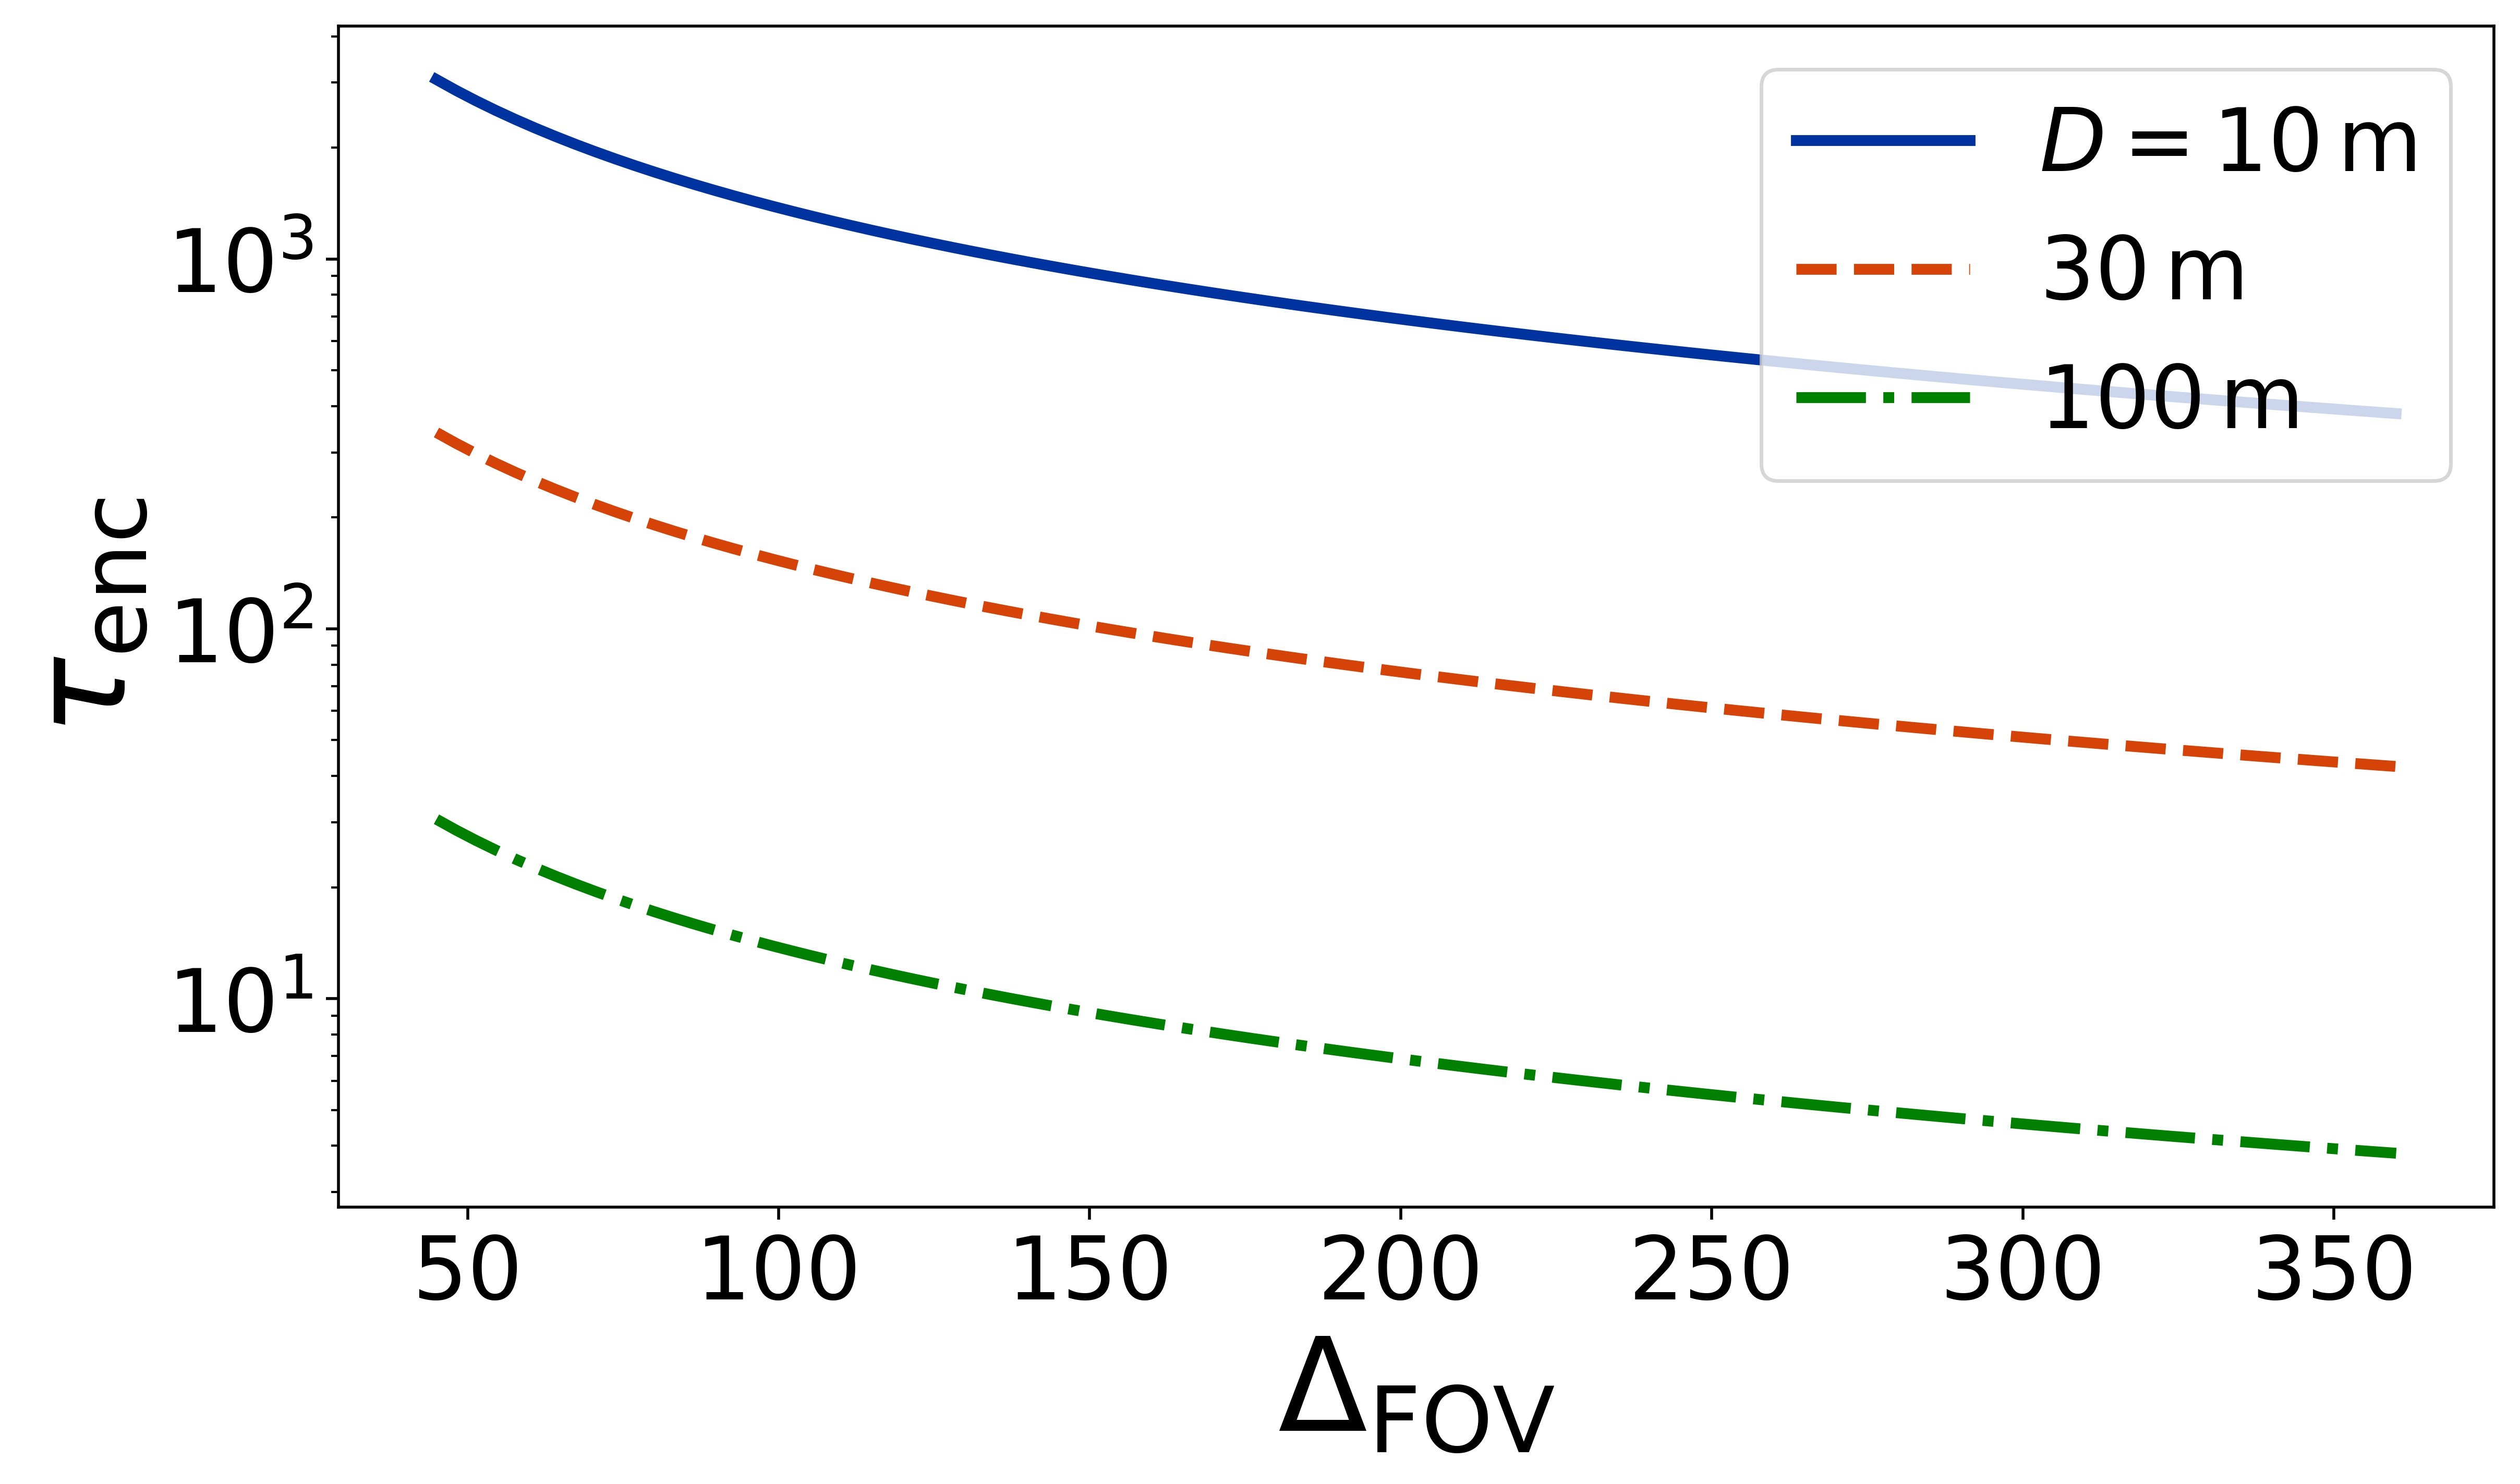
\includegraphics[width=\textwidth]{figures/encounter_time.jpg}
    \caption{The times between dust devil encounters close enough the devils can be clearly resolved for a range of diameters and fields-of-view $\Delta_{\rm FOV}$. All other parameters are the same as in previous figures.}
    \label{fig:encounter_time}
\end{figure}

\section{Assessing the Dust Flux}
Accurate recovery of the dust devil population, in particular the largest devils, may be critical to assess the contribution of dust devils to the martian dust budget. By tracking vertical velocities and optical depths within imaged dust devils, \citet{2006JGRE..11112S09G} estimated dust flux values $q$ for 300 devils, with values ranging between $3.95\times10^{−9}$ and $4.59\times10^{−4}\,{\rm kg\ m^{-2}\ s^{-1}}$ with an average $2.07\times10^{−5}\,{\rm kg\ m^{-2}\ s^{-1}}$, although no information is given regarding the dependence on diameter or any other parameter. Assuming this dust flux applies uniformly across diameter, it suggests the total dust contribution for a devil scales with that devil's areal footprint, i.e.~with $D^2$. We can use these values to explore how well we can estimate the dust flux for a given dust devil population.

Taking the areal occurrence rate of dust devils with a diameter within a small interval around $D$ as $dn/dD = n_0 D^{-\gamma}$ with $\gamma$ between 1 and 2 \citep{2016SSRv..203..277L}. (As before, the area of an individual dust devil does not factor into the areal occurrence rate.) This expression translates into a number of devils observed during a survey of duration $t$ and within a narrow range of diameters $dk/dD = \left( dn/dD \right) A_{\rm survey} t$. Taking the rate of dust mass lifting for a single devil as $Q = q\ \pi D^2$, we can estimate the population-weighted rate as 
\begin{equation}
    Q_{\rm tot} = \int_{D_{\rm min}}^{D_{\rm max}} \left( \frac{dk}{dD} \right) q\ \pi D^2 dD = \int_{D_{\rm min}}^{D_{\rm max}} n_0 D^{-\gamma} \left( \frac{t \Delta_{\rm FOV} D^2}{2 \alpha^2} \right) q \pi D^2\ dD.
    \label{eqn:dust_lifted}
\end{equation}
Although the dust flux $q$ likely depends on $D$ itself, the dependence is unknown, and so for simplicity, we will assume $q = {\rm const.}$, yielding 
\begin{equation}
    \langle Q \rangle = \pi q n_0 \left( \frac{t \Delta_{\rm FOV}}{2 \alpha^2} \right) \left( \frac{D_{\rm max}^{5 - \gamma} - D_{\rm min}^{5 - \gamma}}{5 - \gamma} \right) \approx \left( \frac{ \pi q n_0 }{2 \left( 5 - \gamma \right)} \right) \left( \frac{t \Delta_{\rm FOV}}{\alpha^2} \right) D_{\rm max}^{5 - \gamma},
    \label{eqn:solved_dust_lifted}
\end{equation}
with $\gamma < 5$ and $D_{\rm min} \ll D_{\rm max}$. For a representative estimate, we can take $q = 2.07\times10^{−5}\,{\rm kg\ m^{-2}\ s^{-1}}$, $n_0 = 0.05\,{\rm km^{-2}\ hr^{-1}}$, $\gamma = 1$, $t = 25\,{\rm hrs}$, $\Delta_{\rm FOV} = 65^\circ$, $\alpha = 1\,{\rm mrad}$, and $D_{\rm max} = 100\,{\rm m}$, giving an estimate $\langle Q \rangle \approx 4 {\rm g\ hr^{-1}}$.

\acknowledgments

%% To help institutions obtain information on the effectiveness of their 
%% telescopes the AAS Journals has created a group of keywords for telescope 
%% facilities.
%
%% Following the acknowledgments section, use the following syntax and the
%% \facility{} or \facilities{} macros to list the keywords of facilities used 
%% in the research for the paper.  Each keyword is check against the master 
%% list during copy editing.  Individual instruments can be provided in 
%% parentheses, after the keyword, but they are not verified.

\vspace{5mm}
\facilities{}

%% Similar to \facility{}, there is the optional \software command to allow 
%% authors a place to specify which programs were used during the creation of 
%% the manuscript. Authors should list each code and include either a
%% citation or url to the code inside ()s when available.

\software{}

%% Appendix material should be preceded with a single \appendix command.
%% There should be a \section command for each appendix. Mark appendix
%% subsections with the same markup you use in the main body of the paper.

%% Each Appendix (indicated with \section) will be lettered A, B, C, etc.
%% The equation counter will reset when it encounters the \appendix
%% command and will number appendix equations (A1), (A2), etc. The
%% Figure and Table counter will not reset.

\appendix

\section{Vortex Recovery Statistics}
\label{sec:Vortex Recovery Statistics}
In this section, we describe our analysis of our vortex recovery statistics. We explored the effects of the mean boxcar filter on both the time-series scatter but also on the detected vortices, as well as the effectiveness of our matched filter approach.

For our study here, the mean boxcar filter  acts as high-pass filter on the APSS pressure time-series and, in principle, should induce little distortion on signals much narrower than the filter window size $W$. However, some vortices have quite long durations (many tens of seconds), and so they may be distorted if we use a small enough window. As a measure of this distortion, we can calculate how much less deep a vortex profile would appear after applying the filter by calculating the convolution of a boxcar function against a Lorentzian profile:
\begin{equation}
    \Delta P_{\rm obs}^\prime = \int_{t = -W/2}^{+W/2} \left( \frac{1}{W} \right) \left( \frac{-\Delta P_{\rm obs}}{1 + \left( \frac{t}{\Gamma_{\rm obs}/2} \right)^2} \right) dt = -\left( \frac{\Delta P_{\rm obs} \Gamma_{\rm obs}}{W}\right) \tan^{-1} \left( \frac{W}{\Gamma_{\rm obs}} \right), \label{eqn:tophat_convolution}
\end{equation}
where we have taken the Lorenztian to be centered at $t_0 = 0$ and $\Delta P_{\rm obs}^\prime$ represents the distorted profile depth. Figure \ref{fig:Pobsprime-sigmaP_vs_W}(a) shows the result: for windows more than 100 times the profile's original width (i.e., $W/\Gamma_{\rm obs} > 10^2$), the profile depth is more than 98\% of its original value, indicating minimal distortion. 

Of course, the narrower the window, the more effectively we can reduce the long-term variations in the time-series that may otherwise obscure the vortices. To explore that effect, we applied mean boxcar filters of various widths $W$ to each sol's pressure time-series and then estimated the resulting scatter (via $1.4826\ \times$ the median absolute deviation \citealp{doi:10.1080/01621459.1993.10476408}). Figure \ref{fig:Pobsprime-sigmaP_vs_W}(b) shows that for the time-series for sol 66 exhibited the largest scatter for any value of $W$, while that for sol 30 exhibited the smallest. The time-series for sol 395 had values near the median for all sols. In all cases, as $W$ increases, so does the scatter, consistent with our expectations that less aggressive filtering (i.e., $W$ larger) leaves more noise. We fit Lorentzian profiles to the vortices reported in \citet{2020arXiv200501134S} and found that the largest $\Gamma_{\rm obs} \approx 300\,{\rm s}$. Therefore, we took $W = 3000\,{\rm s}$, meaning that even the most distorted vortices should have $\Delta P_{\rm obs}^\prime/\Delta P_{\rm obs} > 0.8$.

\begin{figure}
    \centering
    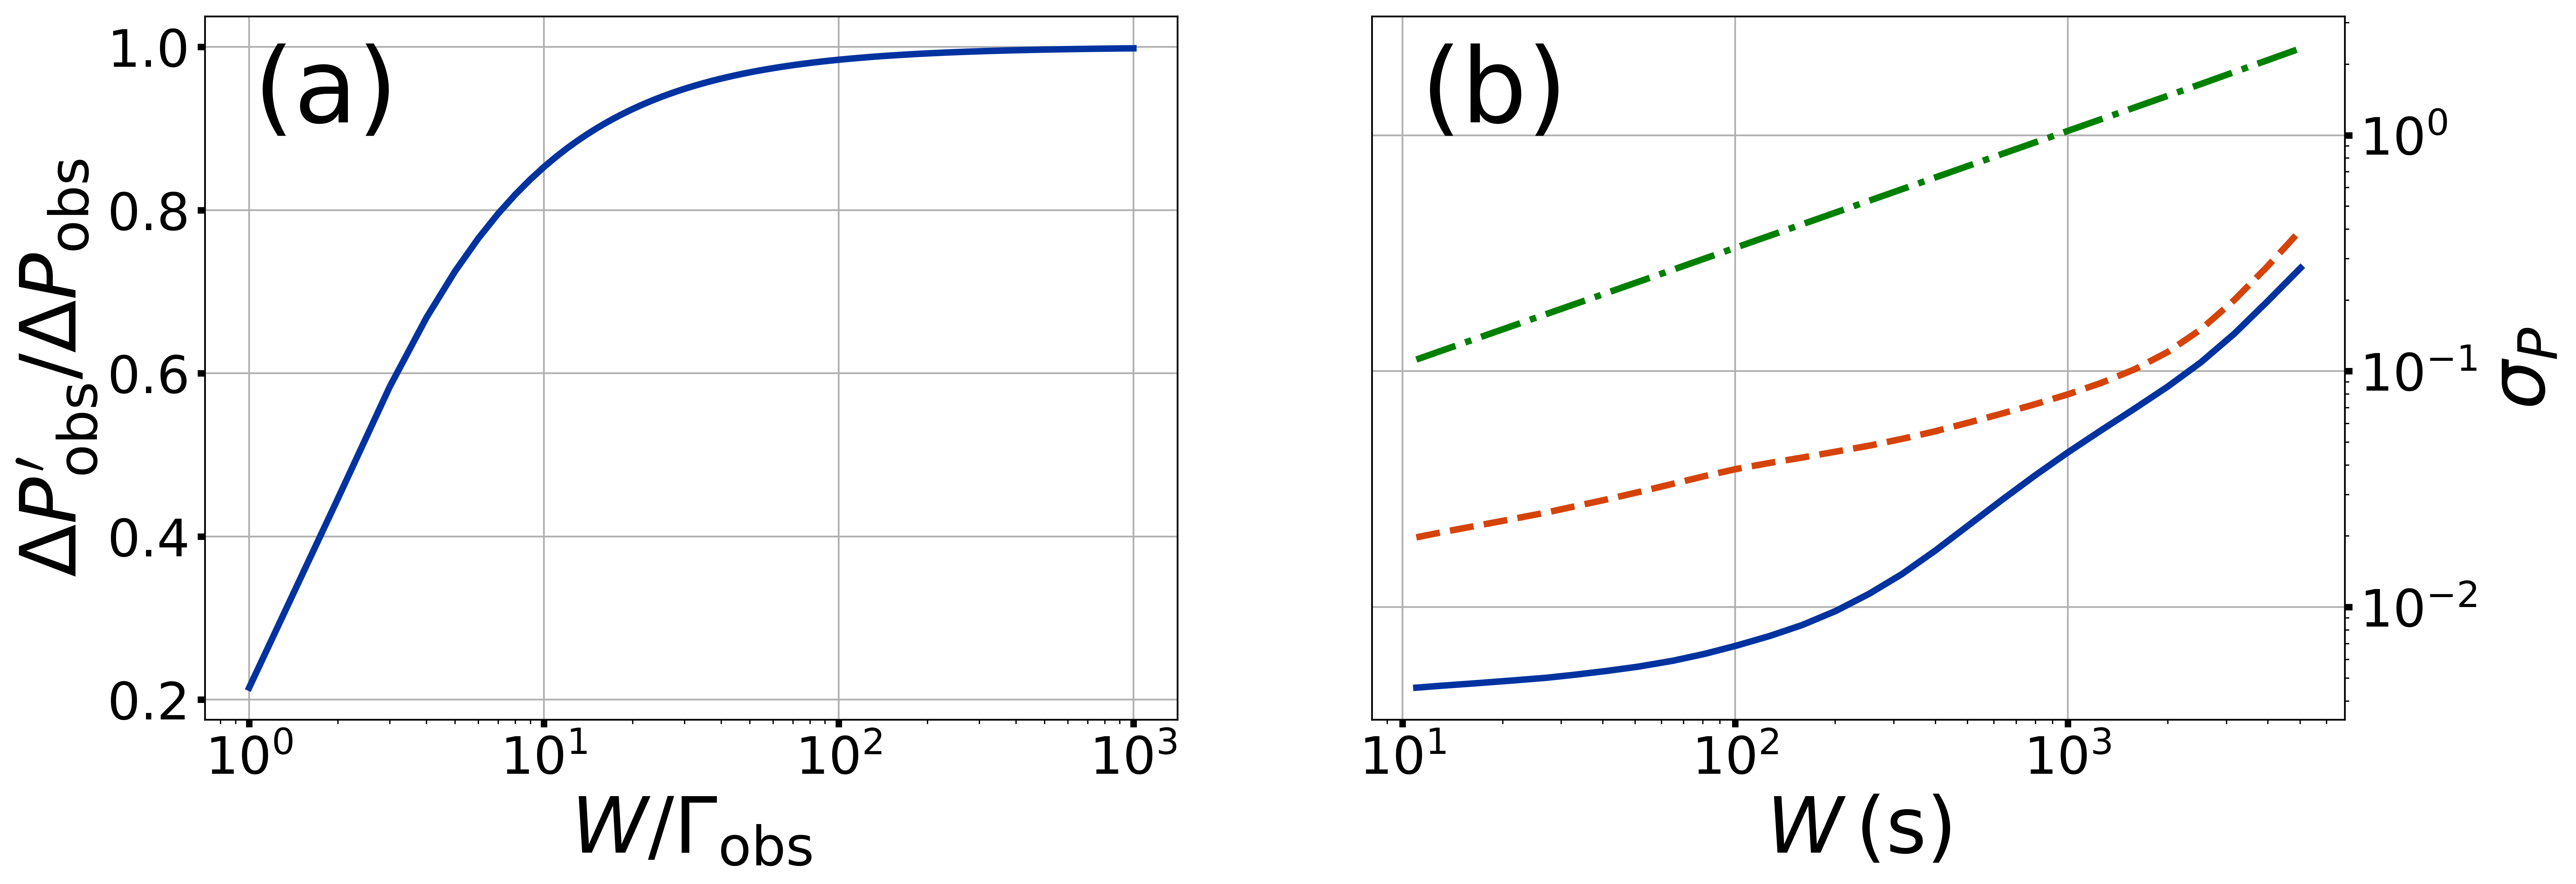
\includegraphics[width=\textwidth]{figures/Pobsprime-sigmaP_vs_W.png}
    \caption{(a) Comparing the pressure excursion observed before $\Delta P_{\rm obs}$ application of the mean boxcar filter and after $\Delta P_{\rm obs}^\prime$ as a function of the width of the filter $W$ and of the vortex signal $\Gamma_{\rm obs}$. (b) Scatter in the pressure time-series $\sigma_P$ for the sol with the largest (sol 435) and least (sol 269) values as a function of the window size $W$ for the mean boxcar filter. Sol 392 has scatter close the median value for all sols. }
    \label{fig:Pobsprime-sigmaP_vs_W}
\end{figure}

Finally, we must interpret these results in terms of our ability to recover vortices using our matched filter approach. In particular, we need to know the best shape for the matched filter: too narrow a filter might miss wider vortex profiles, while a wide filter could average out narrow profiles. To that end, we generated 500,000 synthetic time-series (200 distinct simulations for each of 2500 combinations of model parameters discussed below). These time-series had the same sampling as the APSS time-series and white noise with a wide range of variances $\sigma_\text{P}^2$. Into these time-series, we injected vortex signals with known depths and widths. Then, we applied a matched filter with width $\Gamma$ to see the range of values we retrieved for the convolution of the filter against the synthetic time-series, $\left( F \ast P \right)$. Figure \ref{fig:vortex_recovery} illustrates the range of such values and indicates that, for a very wide range of vortices, noise levels, and matched filter widths, we can successfully recover the vortices. Indeed, Figure \ref{fig:vortex_recovery} shows we could even recover very subtle vortices, given the right filter width. For example, for $\Delta P_{\rm obs}/\sigma_P$ (i.e., a vortex that barely rises above the noise), a wide range of filter widths $\Gamma$ returns $\left( F \ast P \right) \geq 5 $. The noise model discussed here does not include the non-white (red) noise that pervades the real APSS data, meaning the results are somewhat optimistic. However, based on the results here (and on additional experimentation with the real APSS time-series), we chose $\left( F \ast P \right) \geq 5 $ as our vortex detection threshold.

\begin{figure}
    \centering
    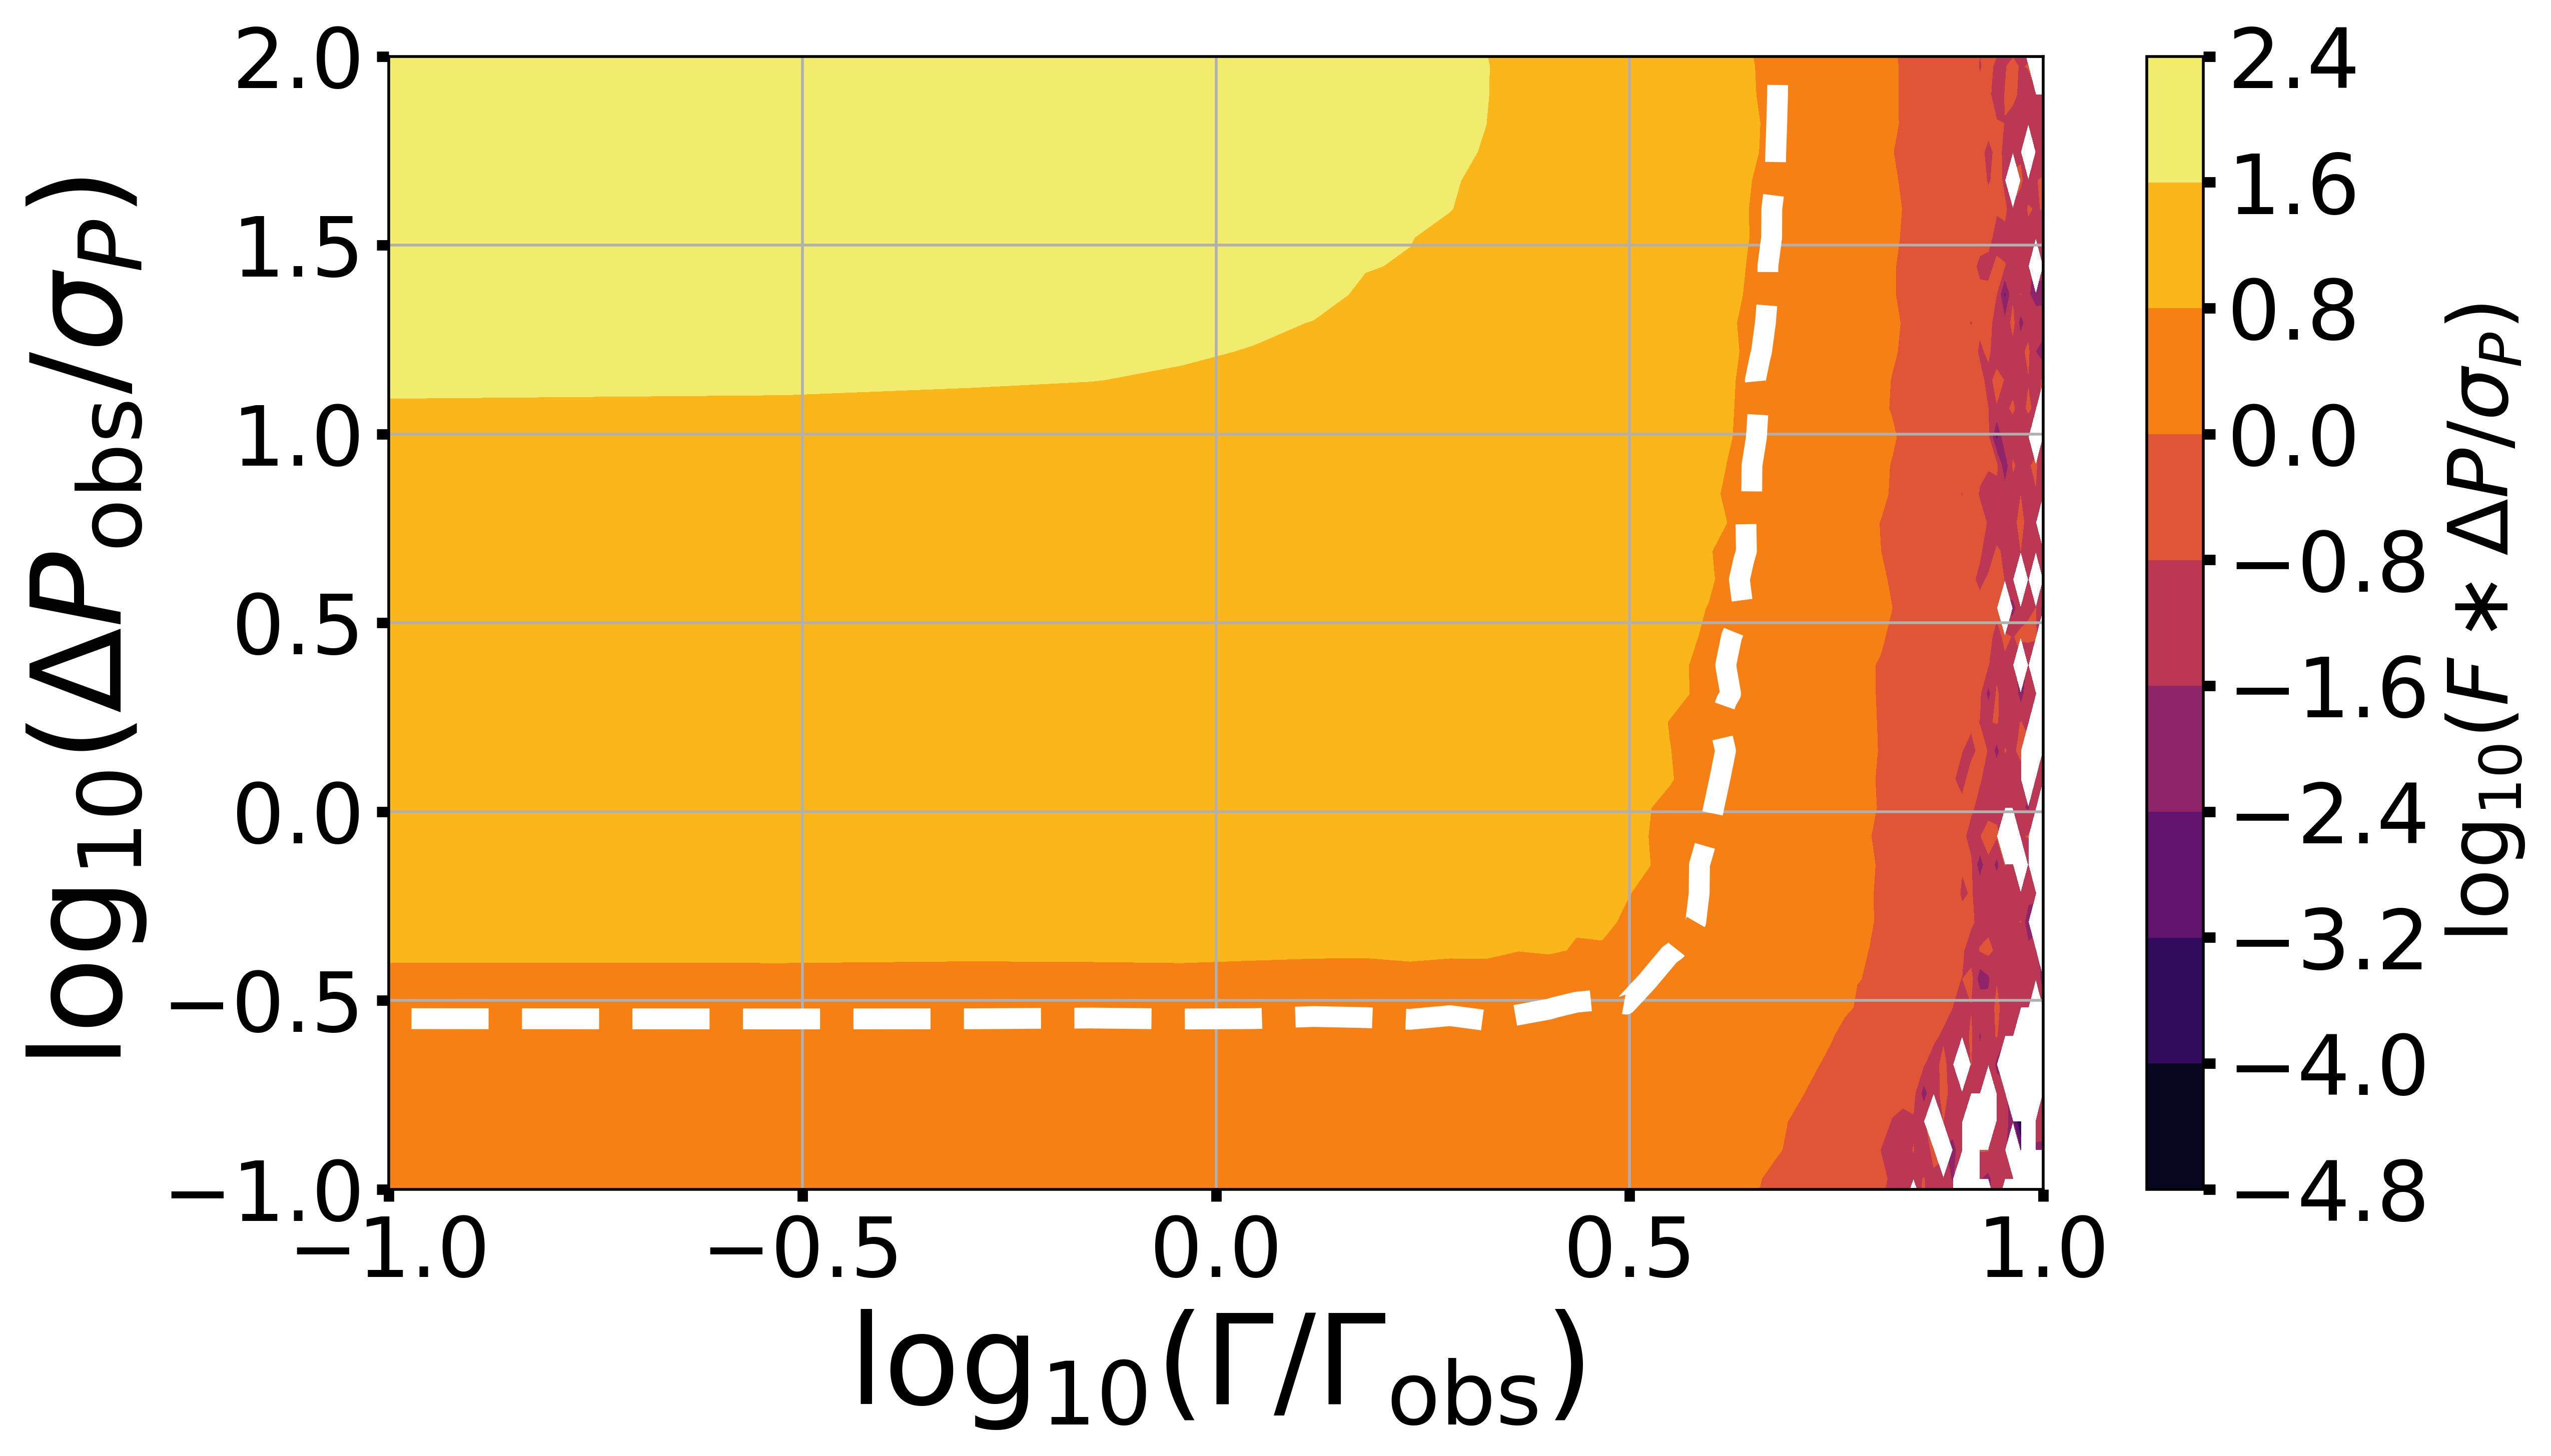
\includegraphics[width=\textwidth]{figures/vortex_recovery.png}
    \caption{How effectively a convolution of a synthetic pressure time-series with the matched filter ($F \ast P$) recovers a vortex. The vortex has a known depth $\Delta P_\text{obs}$ and width $\Gamma_\text{obs}$ and is embedded in a synthetic time-series with white noise of variance $\sigma_\text{P}^2$. The matched filtered has a width $\Gamma$. The dashed, white line shows the threshold for detection used in this study ($F \ast P \geq 5$). In principle, vortices with values of $\Delta P_\text{obs}\sigma_P$ and $\Gamma/\Gamma_\text{obs}$ above and to the left of that line could be recovered.}
    \label{fig:vortex_recovery}
\end{figure}

\section{Inferring Encounter Geometries from the Pressure and Velocity Profiles}
\label{sec:Inferring Encounter Geometries from the Pressure and Velocity Profiles}
We assume the vortices correspond to Rankine vortices \citep{1991ExFl...11...73V}, giving pressure $\Delta P$ and tangential wind velocity profiles $V$:
\begin{equation}
    \Delta P(r) = -\frac{\Delta P_{\rm act}}{1 + \left( \frac{r}{D_{\rm act}/2} \right)^2}\label{eqn:radial_lorentzian_profile}
\end{equation}
and
\begin{equation}
    V(r) = \frac{ V_{\rm act} \left( 2 \frac{r}{D_{\rm act}/2} \right)}{1 + \left( \frac{r}{D_{\rm act}/2} \right)^2},\label{eqn:radial_wind_profile}
\end{equation}
where $r$ is the radial distance from the vortex center, $P_{\rm act}$ the central pressure excursion, and $V_{\rm act}$ the peak velocity at a distance $D_{\rm act}$ from the vortex center. Equation \ref{eqn:radial_distance} shows the evolution of the radial distance with time during an encounter. At closest approach, we measure $\Delta P = \Delta P_{\rm obs}$ (Equation \ref{eqn:Pobs}) and 
\begin{equation}
    V = \frac{ V_{\rm act} \left( 2\frac{b}{D_{\rm act}/2} \right)}{1 + \left( \frac{b}{D_{\rm act}/2} \right)^2} = V_{\rm obs}.\label{eqn:Vobs}
\end{equation} 

Cyclostrophic balance relates the pressure and velocity as \citep{2020Icar..33813523J}:
\begin{equation}
    V_{\rm act} = \left( \Delta P_{\rm act}/\rho \right)^{1/2},\label{eqn:cyclostrophic_balance}
\end{equation}
where $\rho$ is the atmospheric density. Combining Equations \ref{eqn:Pobs}, \ref{eqn:Vobs}, and \ref{eqn:cyclostrophic_balance} gives
\begin{equation}
    \Delta P_{\rm act} = \left( 1 - \frac{\rho V_{\rm obs}^2}{4 \Delta P_{\rm obs}} \right)^{-1} \Delta P_{\rm obs},\label{eqn:solution_for_Pact}
\end{equation}
and
\begin{equation}
    V_{\rm act} = \left( 1 - \frac{\rho V_{\rm obs}^2}{4 \Delta P_{\rm obs}} \right)^{-1/2} \left( \Delta P_{\rm obs}/\rho \right)^{1/2}.\label{eqn:solution_for_Vact}
\end{equation}

We can use these values to infer $b$
\begin{equation}
    b = \left( \frac{D_{\rm act}}{2} \right) \sqrt{\frac{\Delta P_{\rm act}}{\Delta P_{\rm obs}} - 1},
\end{equation}
and then plug this into the relationship between the observed diameter and actual $D_{\rm obs} = \sqrt{D_{\rm act}^2 + \left( 2 b\right)^2 }$ \citep{2020Icar..33813523J}:
\begin{equation}
    D_{\rm act} = \frac{D_{\rm obs}}{\sqrt{\Delta P_{\rm act}/\Delta P_{\rm obs} }}.\label{eqn:actual_diameter}
\end{equation}
We can then use these relationships to solve for $b$.

% For N estimate, with about 6 hours per day of dust devil activity (1/4 day),
%   1 km^{-2} day^{-1} translates into about 0.25 km^{-2}.

% We can compare our estimate for the daily number of vortex encounters and the associated sampling uncertainty from Equations \ref{eqn:number_of_encounters} and \label{eqn:sigma_N} to the actual numbers reported in \citet{2020arXiv200501134S} by plugging in representative values: \citet{2020arXiv200501134S} report typical wind speeds $U \sim 5\,{\rm m\ s^{-1}}$ and vortex activity during about $12\, {\rm hours}$ each sol over about 400 sols; monitoring dust devil tracks around the InSight landing site, \citet{2020GeoRL..4787234P} suggest $N = 0.05\,{\rm km^{-2}\ sol} \times \left(12\,{\rm hours\ sol^{-1}}\right) = 0.025\,{\rm km^{-2}}$ and $D_{\rm act} \approx 10\,{\rm m}$; \citet{2018Icar..299..166J} suggests $P_{\rm act} \approx 1\,{\rm Pa}$; and our analysis here gives $P_{\rm min} \approx 0.3\,{\rm Pa}$. Taken altogether, we estimate InSight could detect vortices out to a distance $b_{\rm max} \approx 8\,{\rm m}$ distance and should have recovered about 

% 2020 May 9 - Check notes in notepad from today's date
% \section{Effects of Undersampling the Dust Devil Profile}
% With too low a sampling frequency, the pressure profile for a dust devil will be undersampled, potentially distorting the inferred profile shape and depth. Fourier analysis of the pressure profile can show the dependence of the distortion on the angular sampling frequency $\omega$.

% We start by assuming a Lorentzian profile $L(t)$ in time $t$ for the dust devil:
% \begin{equation}
%     L(t) = -\frac{\Delta P}{1 + \left( t/\Gamma \right)^2},
%     \label{eqn:appendix_lorentzian}
% \end{equation}{}
% where $\Delta P$ is the profile depth and $\Gamma$ its duration. The Fourier transform of this profile $F(\omega)$ is 
% \begin{equation}
%     F(\omega) = -\pi \Delta P\ \Gamma e^{-|\omega| \Gamma}.
%     \label{eqn:appendix_lorentzian_fourier}
% \end{equation}{}

% If we now imagine that we undersampled the profile using frequencies below some maximum, $\omega \le \omega_{\rm max}$, then we can estimate the resulting distorted profile $L^\prime(t)$ by taking the inverse, partial Fourier transform of $F(t)$, i.e.
% \begin{equation}
%     L^\prime(t) \equiv \int_{\omega = -\omega_{\rm max}}^{\omega_{\rm max}}\ \left( -\pi \Delta P \Gamma e^{-|\omega| \Gamma}\right) \ \left( \frac{e^{+i\omega t}\ d\omega}{2 \pi} \right)
%     = L(t) \bigg[ 1 - \left( \cos \left( \omega_{\rm max} t \right) - \left( \frac{t}{\Gamma} \right) \sin \left( \omega_{\rm max} t \right) \right) e^{-\omega_{\rm max} \Gamma} \bigg].
%     \label{eqn:appendix_inverse_fourier}
% \end{equation}{}

% We expect the register the maximum (in magnitude) pressure excursion at the center of the profile, i.e. $L(t = 0) = \Delta P$, and so to estimate the incorrect profile depth $\Delta P^\prime$ arising from this distorted profile, we can evaluate $L^\prime(t)$ at the same time, giving:
% \begin{equation}
%     \Delta P^\prime = \Delta P \left( 1 - e^{-\omega_{\rm max}\Gamma} \right).
% \end{equation}{}
% The distortion decreases rapidly with $\omega_{\rm max}$, and for a sampling frequency of, for example, $2\,{\rm Hz}$ ($\omega_{\rm max} = 2\pi \times (2\,{\rm Hz})$) and a very narrow profile $\Gamma = 0.5\,{\rm s}$, $\Delta P^\prime$ is only 0.2\% different from $\Delta P$.

\bibliography{sample63}{}
\bibliographystyle{aasjournal}

%% This command is needed to show the entire author+affiliation list when
%% the collaboration and author truncation commands are used.  It has to
%% go at the end of the manuscript.
%\allauthors

%% Include this line if you are using the \added, \replaced, \deleted
%% commands to see a summary list of all changes at the end of the article.
%\listofchanges

\end{document}

% End of file `sample63.tex'.